%%% KCSS Dissertation Template
%%%
%%% Take care of all fields marked <++FOO++>.
%%% When using Vim LaTeX Suite <http://vim-latex.sourceforge.net/>,
%%% then Ctrl-j should navigate to the next such field.

\documentclass[10pt]{book}
\usepackage[language=english,theorems=numbersfirst,paper=a4paper]{ifiseries}
\usepackage{listings}
\usepackage[ruled,vlined]{algorithm2e}
\usepackage{pdfpages}
\usepackage{todonotes}
\usepackage{breakurl}
\usepackage{subcaption}
\usepackage{hyperref}
\usepackage{lipsum}
\usepackage{parcolumns}
\usepackage[printonlyused]{acronym}
\usepackage{bm,amsmath}
\usepackage[newfloat]{minted}
\usepackage{caption}
%\usepackage{mathtools}
\setlength{\marginparwidth}{3cm}
\addbibresource{thesis.bib}

\graphicspath{{./assets/}}

\newenvironment{localsize}[1]
{%
  \clearpage
  \let\orignewcommand\newcommand
  \let\newcommand\renewcommand
  \makeatletter
  \input{bk#1.clo}%
  \makeatother
  \let\newcommand\orignewcommand
}
{%
  \clearpage
}
% Minted env
\newenvironment{code}{\captionsetup{type=listing}}{}
\SetupFloatingEnvironment{listing}{name=Pseudocode}

% \newcommand{\figureref}[1]{\textbf{\autoref{#1}}}
% \newcommand{\figurereft}[2]{\textbf{\autoref{#1} #2}}
\newcommand{\figureref}[1]{\autoref{#1}}
\newcommand{\figurereft}[2]{\autoref{#1} #2}
\newcommand{\toxdo}[1]{}

\newcommand*\NewPage{\newpage\null\thispagestyle{empty}\newpage}

\begin{document}

\frontmatter

\studtitlepage%
{ArUco Marker Detection on Flexible Photonic Crystals}%
{}
{Niklas Carstensen}%
{Master's Thesis}%
{\today}%
{Prof. Dr. Reinhard Koch}%
{Jakob Nazarenus, Tim Michels}%
\NewPage{}
\setcounter{page}{2}
\studeidesstatt
\NewPage{}

\selectlanguage{english}
\setcounter{page}{3}
\chapter*{Abstract}

As part of the development of a medical readout technique, this work addresses the construction of a detection system for \ac{ArUco} marker structures on flexible photonic crystals on tape. For an accurate readout, the camera position relative to the markers is necessary. The task for this work is therefore the development of a robust detection system for the \ac{ArUco} marker corners. With the detected corners, the camera pose can then be computed using already existing technology. The detection task is split into two parts. 

The first part addresses the detection of areas of interest in the image using object detection networks. Due to a shortage of training data, a number of augmentations are defined. 
%The augmentations are prebuilt into the dataset, such that the same augmentation can be tested with many model architectures without changing the dataloader for each one. 
The impact of the augmentations on the resulting \ac{mAP} scores are then measured using ensemble runs and hyperparameter optimizations. Furthermore, inference techniques such as \ac{SAHI} are evaluated and used to increase the detection performance. Despite dissimilarity of training and test data for this part, the augmentation, training and inference techniques can increase the VOC 2010 \ac{mAP} score on test data by more than 60\%. However, those results may not be generalizable.

The second part addresses the detection of the \ac{ArUco} marker corners within the detected area of interest. Here, a number of approaches using keypoint detection, segmentation networks and classic algorithms are tested. Finally, the best performing approach is found using a combination of an U-Net and Hough transform.

\newpage
\section*{Acknowledgements}
Firstly, I want to thank Prof. Dr. Reinhard Koch for giving me the opportunity to write this masters thesis. I also want to thank my advisor Jakob Nazarenus for bringing useful technologies to my attention and Fabio Aldo Kraft for providing the topic as well as the training and test data. Finally I want to thank the entire working group, everyone who participated in the user evaluation, my friends, family and Chodo Habat.

\tableofcontents
\listoffigures
%\listoftodos
\mainmatter
\chapter{Introduction}

There is a global shortage of health workers, that is projected to endure into 2030 \cite{BMJHealthWorkforce22}, while 47\% of available health workers cared for 22\% of the worlds population in 2020. This shortage and unequal distribution of health workers drive the need for more efficient care for patients. 

During treatment, measuring the biomarkers of a patient is essential. However, a common approach for this is the use of label-based quantification methods, which require trained personnel and a laboratory environment. To circumvent this, there are a number of label-free detection concepts \cite{rapp2010biosensors}, one of which is the usage of photonic crystal slabs \cite{Pitruzzello_2018}. Kraft et al. recently showed, that photonic crystal slabs are processable on flexible substrates, which enables an implantation into wound dressing, smart patches or tape \cite{Fab23}.

\begin{figure}
  \caption{Example image of \ac{ArUco} markers on flexible photonic crystals on tape.}
  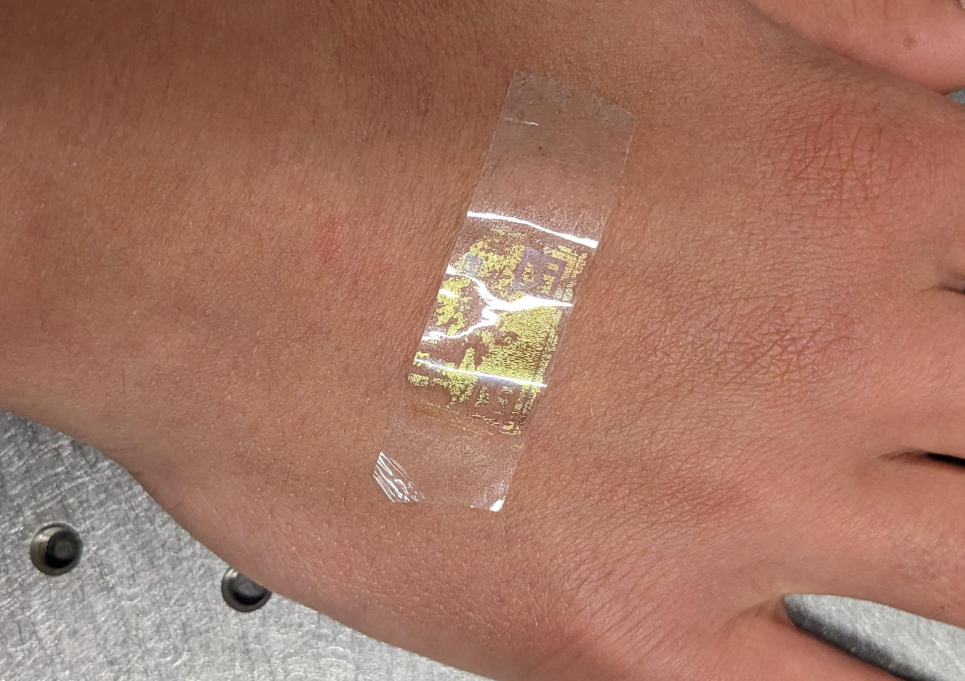
\includegraphics[width=0.65\textwidth]{image/testset_example_crop}
  \label{fig:intro_testset_example}
\end{figure}

However, the optical readout from photonic crystal slabs is challenging, since its optical properties are angle dependant. For the camera of a handheld device, the optical response would therefore change depending on the angle of incidence. To correct this angular readout error, Kraft et al. added \ac{ArUco} fiducial marker structures into the flexible photonic crystal slabs, as seen in \figureref{fig:intro_testset_example}. If printed on paper, these marker structures can be detected and the angle of the marker plane to the camera can be computed by existing software from \ac{OpenCV}. However, the marker structures resulting from the current flexible photonic crystal slab construction process have scratches and are incomplete. Due to this and additional image artifacts, the existing software is not able to detect the marker structures on the flexible photonic crystal slabs.

% A part of the solution for this problem could be small and inexpensive testing equipment \cite{Fab23}, which would allow for fast and regular assessment of ones health without requiring the time of healthcare professionals \cite{POC12}. Such an approach is called \ac{POC}, since the testing and evaluation is done by and of the patient. These kits are also called \acp{POCT}. One type of \ac{POCT} are wearables. However, traditional wearables are based on electrical readout systems \cite{gao2019flexible}, which necessitate conducting wires and a battery and may be invasive. To overcome the drawbacks of wearables using electrical readout systems, optical readout systems can be used instead \cite{nguyen2021wearable}. One approach for an optical readout system is using commercially available adhesive tape, which acts as a \ac{PCS}, and etching \ac{ArUco} fiducial markers into it \cite{Fab23}. This is done by first applying a negative photoresist to the tape and then shining UV light on it, while masking the parts of it that are supposed to become part of the \ac{ArUco} shape later. Then an \ac{IBE} process is applied to the tape and finally the heat resist of the first step is removed during an ultrasonic heat bath.

\section{Problem Statement}

The goal of this work is to find a new detection process which has less sensitivity to artifacts in the \ac{ArUco} fiducial marker structures. 
%For this, different algorithmic detection approaches are analyzed. 
Since the tapes should be used by patients, the technology developed here is supposed to run on patients smart phones. While smart phones are easily carryable, they come with the drawback of not having much space or energy for large \acp{GPU}, which limits the choice of neural network models.

\section{Outline}

Firstly, \autoref{chap:prelim} introduces important definitions and used technologies. Afterwards, \autoref{chap:relatedw} discusses how similar problems of difficult \ac{ArUco} marker detection and image augmentation design were solved in other papers. \autoref{chap:netw} introduces the used network architectures with special focus on \ac{YOLO}. \autoref{chap:implement} covers the most relevant parts of the development of the software and the model training. \autoref{chap:eval} evaluates the approaches discussed before using the software from the previous chapter, compares the results to the results of a small human study and discusses the results. Finally, \autoref{chap:conclusion} concludes the thesis and introduces yet unsolved problems which may be addressed in future work.

\chapter{Preliminaries}
\label{chap:prelim}

The later chapters of this thesis are based on a number of technologies, concepts, definitions and terms, which are introduced here.

\section{Definitions}

The term dataset\footnote{\url{https://en.wikipedia.org/wiki/Data_set}, accessed on 01.10.2023} is central to machine learning as it defines what is fitted to. However, this term is ambiguous as it describes both a list of images and labels\footnote{\url{https://pytorch.org/tutorials/beginner/introyt/trainingyt.html}, accessed on 01.10.2023}, as well as a set of lists of images and labels \cite{lin2014microsoft}. In other subfields of machine learning, a dataset may contain different data types other than images. For this thesis, however, dataset and similar terms are defined as follows:

\begin{description}
  \item[Label] A \textit{label} or \textit{annotation} refers to extra data that belongs to an image and describes a subset of the images contents. \textit{Labels} are usually created using human input and describe the desired output of a machine learning model on that image.
  \item[Data Instance] A \textit{data instance} refers to a tuple of an image and a label.
  \item[Dataseries] A \textit{dataseries} refers to a list of \textit{data instances}.
  \item[Dataset] A \textit{dataset} refers to a set of up to three \textit{dataseries}.
  % \item[Datagroup] A \textit{datagroup} refers to a \textit{dataseries} in the context of a \textit{dataset}. Typical \textit{datagroups} are 'training', 'validation' and 'testing' or 'train', 'val' and 'test' for short.
\end{description}

\section{Neural Networks}

This section gives a brief overview over \acp{ANN}. Since this thesis is written from a computer science perspective, the term \acp{NN} is used interchangeably with \acp{ANN}.

\subsection{History}

Neural network interest and research happened in waves over the last decades, starting with McCulloch and Pitts' work on logical operations on neurons in 1943 \cite{mcculloch1943logical,485891}. 

\begin{figure}
  \caption{Visualization of a perceptron.}
  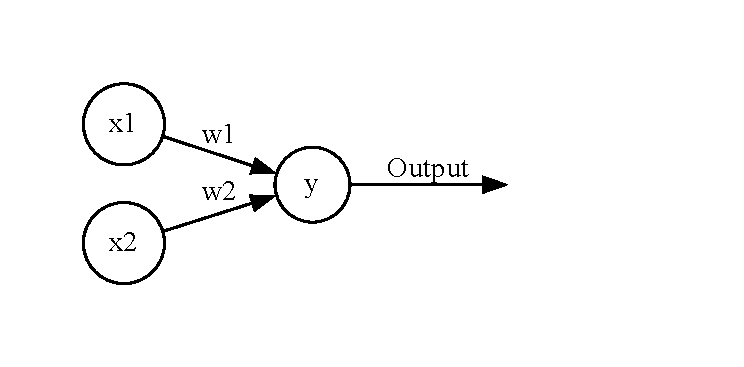
\includegraphics[width=0.48\textwidth]{graph/rosenblatt}
  \label{fig:perceptron}
\end{figure}

The second wave started in the early 1960ies with Rosenblatt's perceptron convergence theorem \cite{rosenblatt1962principles}. A visualization of the perceptron can be seen in \figureref{fig:perceptron} and the output of the perceptron is calculated as follows:
\[
    p(x)= 
\begin{cases}
    1, & \text{if } \sum_i w_ix_i + b > 0\\
    0, & \text{otherwise}
\end{cases}
\]
Setting $w1$ and $w2$ to 1 yields a perceptron that implements the logical or operation. As McCulloch and Pitts' work showed, the perceptron is able to model all simple logical operations such as: and, or, not. However, the second wave slowed as Minsky and Papert showed that the perceptron is unable to model the XOR operation \cite{minsky1969perceptron} even though the \ac{MLP} seen in \figureref{fig:mlp} that Rosenblatt already proposed at the time could model XOR through the combination of multiple perceptrons \cite{schmidhuber2022annotated}.

The third and ongoing wave started in the early 1980s with Hopfield's energy approach \cite{hopfield1982neural} as well as the introduction and refinement of back-propagation for \acp{MLP} \cite{werbos1974beyond,rumelhart1986parallel}.

\subsection{CNN}

\begin{figure}
  \caption{Visualization of a \ac{MLP}.}
  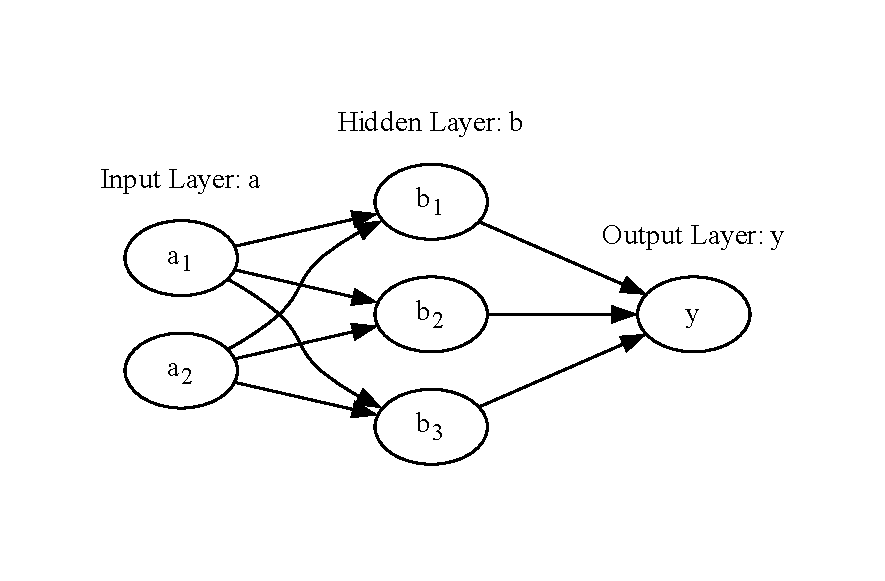
\includegraphics[width=0.48\textwidth]{graph/mlp}
  \label{fig:mlp} 
\end{figure}

Each node in b in the \ac{MLP} as seen in \figureref{fig:mlp} is calculated like the node y in \figureref{fig:perceptron}. That also means that every node combination between the layers has a weight. Such a combination of layers is called a fully connected layer. If there is a high degree of correlation between all the nodes, then such a fully connected layer is useful as it is also fully utilized. However, particularly when the nodes of the input layer represent the pixels of an image and the task is some form of recognition of objects in the image, most connections are not well utilized since pixels that are further away from each other tend to have no meaningful connection \cite{aghdam2017guide}.

Convolutional layers work like a kernel-based image filter but make the kernel trainable instead of static. This has the advantage that each convolutional neuron only processes data from its receptive field instead of the whole image. The receptive field of a neuron refers to the area of pixels in the source image that the input data of the neuron is dependent on. Using just one convolutional layer means that the neurons in the resulting tensor are just dependent on an area in the source image as big as the kernel of that convolution. Therefore, \acp{CNN} tend to have many layers to be able to recognize larger shapes in the image. The resulting data of a convolutional layer is also called a feature map. 

\section{Shapely} % TODO: Add cites or footnotes in these sections

Shapely is a popular Python package for computational geometry\footnote{\url{https://shapely.readthedocs.io/en/stable/manual.html}, accessed on 16.12.2023}. It provides a wide range of geometric objects and operations for working with planar geometric shapes, such as points, lines and polygons. Shapely is widely used in various domains, including geographic information systems, spatial data analysis, and computer graphics.

\section{Open CV}

\ac{OpenCV} is an open-source computer vision and machine learning software library designed for various computer vision tasks such as image processing and object detection\footnote{\url{https://opencv.org}, accessed on 16.12.2023}. It was originally developed by Intel and later maintained by Willow Garage and Itseez. \ac{OpenCV} is written in C++ and has interfaces for C++, Python, and other programming languages.

\subsection{ArUco Detection}
\label{sec:aruco_det}

The \ac{ArUco} detector implemented into \ac{OpenCV} is based on a paper from Garrido-Jurado et al. \cite{garrido2014automatic}. The \ac{ArUco} detection starts by using local adaptive thresholding on the image. Afterwards the Suzuki
and Abe algorithm \cite{SUZUKI198532} is applied to the thresholded image to extract the contours. The contours are then transformed into polygons using the Douglas-Peucker algorithm \cite{douglas1973algorithms} and all polygons with more or less than 4 vertices are discarded. Then homographies for all remaining polygons are calculated such that the perspective on the potential marker can be removed. The flattened image is then binarized using Otsu's method \cite{4310076}, which results in the lowest possible intra-class variance of black and white parts of the potential marker. Finally, the marker is divided into a grid and further processed as a binary number based on the brightness of the grid cells.

This algorithm is, however, based on the assumption that the marker contours are always visible. If they are not, detections can become skewed or nothing is detected, as seen in \figureref{fig:aruco-det}.

\begin{figure}
  \centering
  \subcaptionbox{An easily detectable \ac{ArUco} marker image}
     {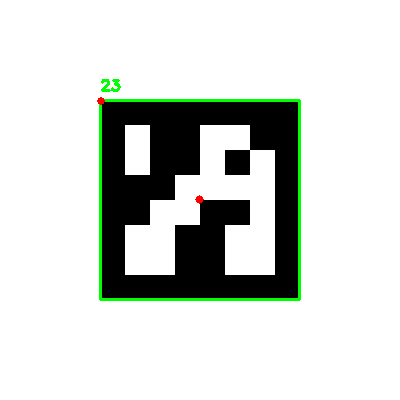
\includegraphics[width=0.31\textwidth]{image/rec}}
  \subcaptionbox{An \ac{ArUco} marker image with obscured contour corner}
     {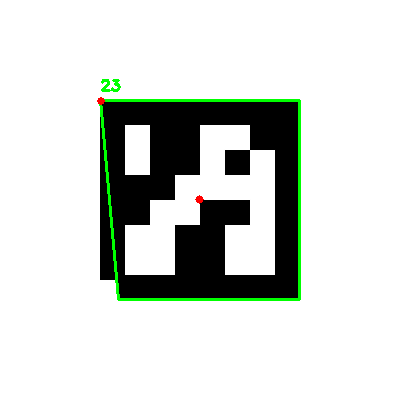
\includegraphics[width=0.31\textwidth]{image/skewed-rec}}
  \subcaptionbox{An \ac{ArUco} marker image with broken contour}
     {
\includegraphics[width=0.31\textwidth]{image/no-rec}}
  \caption{Open CV ArUco Detection on example \ac{ArUco} images which have been partly obscured by a white rectangle.}
  \label{fig:aruco-det}
\end{figure}

\section{Albumentations}

Albumentations is a Python library for image augmentation\footnote{\url{https://albumentations.ai}, accessed on 16.12.2023} \cite{info11020125}. Image augmentation is a technique used to artificially expand a dataset by applying various transformations to the existing images. This helps improve the performance and generalization of machine learning models, especially in scenarios where the training data is limited. 

Albumentations was primarily built for high performance, such that its usage in dataloaders does not slow down the training process \cite{info11020125}. It transforms the image, as well as the keypoint, bounding box and mask labels of the training data, if the selected augmentation transformations support the label format. 

\section{Pytorch}

PyTorch is an open-source machine learning library for Python that has gained significant popularity in the deep learning and artificial intelligence research communities\footnote{\url{https://albumentations.ai}, accessed on 16.12.2023}. It was originally developed by Facebook's AI Research lab (FAIR) and is now maintained by the Linux Foundation. %PyTorch offers a flexible and dynamic computational graph, making it particularly well-suited for developing and training neural networks.

\section{SAHI}

The Python package \ac{SAHI} is a lightweight vision library designed to perform large scale object detection and instance segmentation \cite{akyon2022sahi,obss2021sahi}. It was developed to address the challenges of detecting small objects and performing inference on large images, which are common issues in the practical usage of object detection models. 

Fundamentally, \ac{SAHI} uses a sliding window over the input image to split it into slices and lets the model predict objects in each of the slices of the image individually. Then, it combines the predictions done on image slices into a prediction over the whole image. Since the slices may overlap, there is support for bounding box prediction combination. Since models only support input images at a fixed resolution and smaller objects may disappear if the image is rescaled, this sliding window approach helps with detection on large images or of smaller objects.

\ac{SAHI} is framework agnostic and therefore can be modified to work with any model. However, it has \ac{YOLO}X, \ac{YOLO}v5, \ac{YOLO}v8, MMDetection and Detectron2 support by default.

\section{HyperOpt}

Hyperopt is a Python package designed for hyperparameter optimization, a fundamental aspect of machine learning model development \cite{bergstra2013making}. It systematically explores the hyperparameter space using a variety of optimization algorithms, such as \ac{TPE}, aiming to discover the parameter combination that optimizes a predefined objective function. %In this context, hyperparameters refer to extra parameters of the machine learning training process, which determine the performance of the trained model.

Hyperopt sees the objective function as a black box and makes few assumptions, which comes with flexibility but slower optimization than with loss functions in neural network training. Since an entire machine learning training run is not a derivable function, this is the best choice for optimizing hyperparameters.

A combination of grid search and manual search is widely used to optimize hyperparameters. However, it was shown that such processes tend to not be as efficient as sampling randomly from the hyperparameter space \cite{bergstra2012random}. \ac{TPE} is based on this realization, as it behaves like random sampling in the first runs. However afterwards, it uses the sampling history to find promising new parameter combinations \cite{bergstra2011algorithms}. 
% \ac{TPE} roughly works in these steps:

% \begin{enumerate}
%   \item Initialize the search space with Gaussian distributions or categorical distributions for continuous parameters and discrete parameters respectively.
%   \item Sample the objective function
%   \item The outputs of the objective function are thresholded into good and bad configurations
%   \item A exploitation \ac{PDF} is constructed for good configurations and a exploration \ac{PDF} is constructed for bad configurations
%   \item 
% \end{enumerate}

% TODO?: \section{Bounding Box conventions}

\section{mAP Scores}

\ac{mAP} scores are a class of commonly used metrics in the field of object detection. They help evaluate the performance of an object detection model \cite{padilla2020survey} and aim to provide a measure of how well the model can identify and locate objects within an image. However, there is a lack of consensus about the \ac{mAP} calculation. I will therefore focus on three popular \ac{mAP} scores. 

\subsection{IoU}

\begin{figure}
  \caption{Visualization of \ac{IoU} calculation.}
  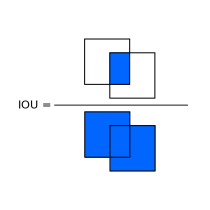
\includegraphics[width=0.5\textwidth]{image/iou}
  \label{fig:iou}
\end{figure}

The metric commonly chosen to measure the prediction quality between a prediction and ground truth label is the \ac{IoU} \cite{padilla2020survey}. The \ac{IoU} is a measurement based on the Jaccard Index, a coefficient representing the similarity of two sets of data \cite{jaccard1901etude}. In the object detection context, the \ac{IoU} measures the area of overlap divided by the area of union between two bounding boxes, as shown in \figureref{fig:iou}. It therefore describes how tight a prediction bounding box is fitted around a ground truth bounding box.

\subsection{Precision and Recall}

In the context of object detection, there are three prediction cases. \ac{TN} is omitted here since it applies to all possible bounding boxes that were not predicted. It therefore depends more on the image resolution than the predictions, assuming the bounding box coordinates are integer values.

\begin{itemize}
  \item[$\bullet$] \ac{TP}: The highest confidence prediction of a ground truth label with an \ac{IoU} higher than the threshold
  \item[$\bullet$] \ac{FP}: An incorrect or imprecise prediction
  \item[$\bullet$] \ac{FN}: An undetected ground truth bounding box
\end{itemize}

Since \ac{TN} is not available in this context, metrics that use the \ac{TN} are also not available \cite{padilla2020survey}. Instead, precision $P$ and recall $R$ are used as metrics.

$$P = \frac{TP}{TP + FP} = \frac{TP}{\text{all predictions}}$$

$$R = \frac{TP}{TP + FN} = \frac{TP}{\text{all ground truths}}$$

Precision measures the percentage of correct predictions among all predictions and recall measures the percentage of correct predictions among all ground truth boxes. 

The difference between the scores becomes most apparent when thinking about the extreme cases. If a model would output every possible bounding box on an image, the recall would be 100\% since for each ground truth bounding box there is an exact same prediction bounding box. If a model would instead output a perfect prediction for one ground truth bounding box and nothing for any of the other ground truth bounding boxes, the precision would be 100\% since each prediction is correct. Since both cases are undesirable but still result in a high score in one of the metrics, a combination of both is needed.

\subsection{Table}

\begin{figure}
  \caption{Visualization of example prediction and ground truth bounding boxes.}
  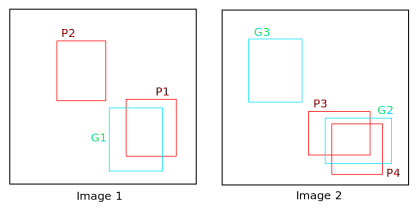
\includegraphics[width=0.8\textwidth]{image/preds}
  \label{fig:preds}
\end{figure}

The first part of the \ac{mAP} calculation is the same across all scores considered. That unified part of the computation is described here using the example\footnote{\url{https://kharshit.github.io/blog/2019/09/20/evaluation-metrics-for-object-detection-and-segmentation}, accessed on 08.10.2023} shown in \figureref{fig:preds}. 

Firstly, a table of all predictions over all images in a given dataseries is created, as seen in Table \ref{tab:mAP}. The table is sorted by prediction confidence. If there are multiple predictions for a single ground truth label, the prediction with the highest confidence is considered TP if its \ac{IoU} is over the threshold and all others are FP, as seen with prediction P3.

\begin{table}
  \begin{tabular}{ c c c c c c c c }
   Ground truth & Prediction & Confidence & TP & Acc. TP & Acc. FP & Precision & Recall \\ 
   \hline
   G2 & P4 & 98\% & Yes & 1 & 0 & 1 & 0.33 \\
   G2 & P3 & 89\% & No & 1 & 1 & 0.5 & 0.33 \\
   G1 & P1 & 78\% & Yes & 2 & 1 & 0.67 & 0.67 \\
   - & P2 & 60\% & No & 2 & 2 & 0.5 & 0.67 \\
   \hline
  \end{tabular}
  \caption{\label{tab:mAP}\ac{mAP} table of the example given in \figureref{fig:preds}.}
\end{table}

As the table is stepped through from the highest confidence predictions to lowest, the accumulated \ac{TP} and \ac{FP} are incremented based on whether the prediction was correct or incorrect and saved into each table row \cite{padilla2020survey}. By dividing the accumulated \ac{TP} by the number of visited table rows so far, a preliminary precision is computed for each row. Similarly, a preliminary recall value is calculated for each table row by dividing the accumulated \ac{TP} by the total number of ground truth labels of all images. Due to their computation formula here, recall values are monotonically increasing as the table rows are visited. However, precision values can both decrease and increase since both the numerator and denominator of the division change. When plotting the precision and recall values of the table rows as y and x components of points, the \ac{PR curve} is obtained, as seen in \figureref{fig:pr-curve}.

\begin{figure}
  \caption{Example of a \ac{PR curve} plot taken from training with real data.}
  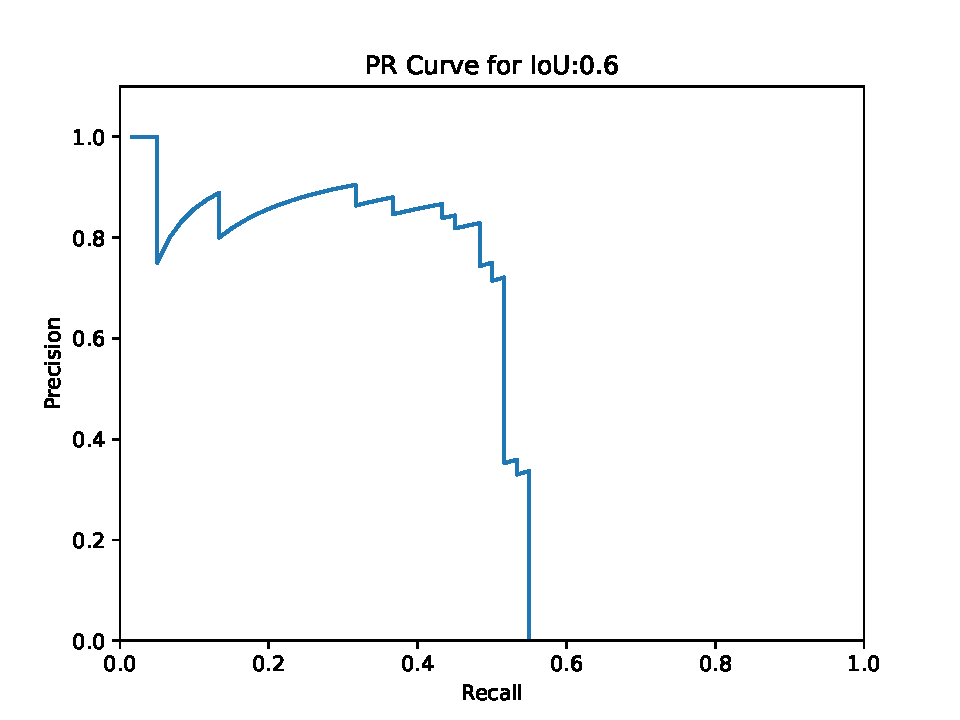
\includegraphics[width=0.8\textwidth]{image/eval_PR_Curve_0.60}
  \label{fig:pr-curve}
\end{figure}

The \ac{mAP} scores are now based on the \ac{AUC} of the \ac{PR curve}, which represents the desired combination of the precision and recall scores.

\subsection{Pascal VOC 2007}

For the VOC 2007 score, the table as described earlier is computed for an \ac{IoU} threshold of 0.5 \cite{everingham2010pascal}. This threshold is deliberately set low to account for inaccuracies in the ground truth data that can arise from hard-to-label objects. The VOC 2007 score summarizes the shape of the \ac{PR curve} by taking 11 equally spaced recall values. For each chosen recall value, the maximum precision value on the curve at or to the right of that recall value is computed. Finally, the AP score is defined as the mean of those maximum precision values, as given by:

$$AP_{11} = \frac{1}{11} \sum_{r\in(0,0.1,...,1)}p_{interp}(r)$$

where

$$p_{interp}(r) = max_{\bar{r} : \bar{r} \geq r}p(r)$$

%$$p(r) = \text{the precision value on the \ac{PR curve} given a recall value}$$

Since I focus on the one class case for object detection, e.g., only on ArUco markers, that AP score is also the \ac{mAP} score here. Otherwise, the \ac{mAP} score would be the mean of the AP scores of all classes.

\subsection{Pascal VOC 2010}

The VOC 2010 score computes the \ac{PR curve} for an \ac{IoU} threshold of 0.5. It considers the \ac{PR curve} \ac{AUC} not just at 11 points but on all points of the table, giving this approach the name all-point interpolation \cite{padilla2020survey}. It is computed using the following formula:

$$AP_{all} = \sum_{n}(r_{n+1} - r_n)p_{interp}(r_{n+1})$$

where

$$p_{interp}(r_{n + 1}) = max_{\bar{r} : \bar{r} \geq r_{n+1}}p(\bar{r})$$

Since the VOC 2010 score takes all given recall values into account, it is generally more accurate than the VOC 2007 score.

\subsection{Microsoft COCO}

The object detection part of the \ac{COCO} detection challenge defines multiple AP score types, such as AP across scales, in which the ground truth masks are split by their pixel area \cite{padilla2020survey}. However, for this work I focused on the AP@50:5:95 score of \ac{COCO}, which I refer to as the \ac{COCO} \ac{mAP} score in the following unless further specified. The \ac{COCO} \ac{mAP} refers to the computation of multiple \acp{PR curve} using different \ac{IoU} thresholds. In this case 10 \ac{IoU} thresholds from 0.50 to 0.95 with a step width of 0.05 \cite{terven2023comprehensive}. \ac{COCO} also uses recall points similarly to the VOC 2007 score. However, with 101 values instead of 11 between 0 and 1 with a step width of 0.01. %given by the following number series: ${0, 0.01, ..., 1}$. 
The \ac{COCO} \ac{mAP} score or average mean average precision score as proposed by Redmon et al. then refers to the average of the computed \ac{mAP} scores for each \ac{IoU} threshold \cite{redmon2018yolov3}. 

The \ac{COCO} \ac{mAP} scores usefulness lies in its measurement of how tight a prediction bounding box is around a ground truth bounding box by using higher \ac{IoU} thresholds. Both VOC scores described earlier see a prediction as correct as soon as its \ac{IoU} is above 0.5 and make no difference between predictions with an \ac{IoU} of 0.55 or 0.9. The \ac{COCO} score therefore gives the opportunity to measure further improvements to trained models, assuming the ground truth labels of the dataset are accurate enough.

\chapter{Related Work}
\label{chap:relatedw}

In the following paragraphs, papers focusing on challenging \ac{ArUco} marker detection using neural networks, as well as papers focusing on image augmentation techniques, are shortly introduced.

\section{ArUco Marker Detection}

In most use cases, \ac{ArUco} markers can be detected by the \acp{OpenCV} detection algorithm. However, there are a number of more challenging use cases. In the following some of them shortly introduced.

\subsection{UAV pose estimation}

Another use case in which robust detection of \ac{ArUco} markers is essential, is for the control of \acp{UAV} during landing \cite{li2020aruco}. Here, camera pose estimation can help locate the \ac{UAV} if \ac{ArUco} markers are layed out on the landing field. However during real world usage, markers can become occluded. Furthermore, other visual artifacts can make detection difficult. Therefore, Li et al. used fine tuned versions of \ac{YOLO}v3-spp and \ac{YOLO}v3-tiny as marker detectors, since these \ac{CNN} based detection systems can be more robust than classic detection systems. For training, the \ac{UAV} took off, floated and landed repeatedly and images were taken. The original $4000 \times 2250$ pixel images were resized to $1000 \times 562$ pixel for higher subsequent processing speed. To make the training data more realistic, black and white objects were placed on the floor to simulate occluding objects. For the test set, images were taken similarly, but markers were partly occluded by laying a white paper cutout on top of it with occlusion ratios from 10\% to 40\%. 

Markers in test images which had occluded borders still had high detection rates even at high cover ratios, while markers with an occluded middle had worse detection rates. This shows that the marker pattern itself was most important for the detection in this case \cite{li2020aruco}.

\subsection{Deep ChArUco}

%Other papers, which focus on neural network aided detection of \ac{ArUco} markers, do not address occlusion. However, 
Hu et al's paper on ChArUcoNet and RefineNet covers keypoint detection of the marker corners in an postprocessing step after the bounding box detection under low light conditions \cite{hu2019deep}. Therefore, the augmentations also focus on noise, blur and brightness as well as shadow effects and a homographic transform. Deep ChArUco is able to detect the markers reliably even at higher darkness degrees while the \ac{ArUco} detection algorithm fails earlier. 

\subsection{Helping people with visual impairment}

Elgendy et al. propose a navigation system for people with visual impairment using \ac{ArUco} markers which are placed indoors \cite{elgendy2021novel}. A series of modified networks which are all based on \ac{YOLO}v3-tiny were trained on 600 photos, which were expanded and augmented on disk to 7200 images. The augmentations used here include 90 degree rotation, blur and lighting effects. The evaluations showed high detection accuracies with higher accuracies on the custom \ac{YOLO}v3 networks. The networks were also successfully deployed on a HTC Desire 826.

\section{Training Image Augmentation}

Image Augmentation is of large importance for generalization. Since a model is build in training by optimizing the similarity of its output on training images to target output, it will also only perform well on examples it was trained on or that are similar. Through variation in training, models can attain a level of generalization that allows them to perform well despite differences in lighting, occlusion, background, scale and so on \cite{shorten2019survey}. A lack of such an ability of generalization leads to previously working models being unable to classify images if a single pixel changes color \cite{8601309}. Often, this variation can come from a large dataset, but if real data is in short supply or if the labeling is too time consuming, image augmentation can replace it to some degree.

Image augmentations can be any kind of image transformation. However depending on the task and the dataset, the effectiveness of different types of augmentations can vary. Nonetheless, in the following I will introduce available papers with empirical comparisons or meta analyses of image augmentations.

\subsection{Comparison of augmentations on the Caltech101 dataset}

On the Caltech101 dataset using a custom classification \ac{CNN}, Taylor et al. found that cropping improves the accuracy scores significantly while most other types of augmentation including custom augmentation types improve the score slightly as seen in Table \ref{tab:taylor-acc} \cite{8628742}. % TODO: Explain the accuracy scores here

\begin{table}
  \begin{tabular}{ c c c }
    & Top-1 Accuracy & Top-5 Accuracy \\ 
   \hline
   Baseline & $48.13 \pm 0.42\%$ & $64.50 \pm 0.65\%$ \\
   Flipping & $49.73 \pm 1.13\%$ & $67.36 \pm 1.38\%$ \\
   Rotation & $50.80 \pm 0.63\%$ & $69.41 \pm 0.48\%$ \\
   Cropping & $61.95 \pm 1.01\%$ & $79.10 \pm 0.80\%$ \\
   Color Jittering & $49.57 \pm 0.53\%$ & $67.18 \pm 0.42\%$ \\
   Edge Enhancement & $49.29 \pm 1.16\%$ & $66.49 \pm 0.84\%$ \\
   Fancy PCA & $49.41 \pm 0.84\%$ & $67.54 \pm 1.01\%$ \\
   \hline
  \end{tabular}
  \caption{\label{tab:taylor-acc}Results of augmentation comparison from Taylor et al. \cite{8628742}.}
\end{table}

\subsection{Comparison of augmentations for detection of COVID-19 Pneumonia}

For automated detection of COVID-19 pneumonia in Chest X-rays, Elgendi et al. empirically tested different combinations of augmentations from other related papers on three datasets 
%with 10-fold cross validation 
of Chest X-ray images \cite{elgendi2021effectiveness}. They used 17 different pretrained neural network models for transfer learning on this binary classification task. For each set of augmentations, they trained the 17 models using that set of augmentations and scored the augmentation set based on the average score of those 17 models. The following augmentations were considered:

\begin{itemize}
  \item[$\bullet$] Reflection
  \item[$\bullet$] Scaling
  \item[$\bullet$] Shearing
  \item[$\bullet$] Translation
  \item[$\bullet$] Rotation
\end{itemize}

While not using any augmentations led to the best score for this task, an augmentation pipeline consisting of reflection, translation and rotation got the second best score. The worst score was attained by an augmentation pipeline consisting of shearing, translation and rotation. 

Elgendi et al. also asked radiologists whether the augmentations used here made sense in the context of pneumonia detection and the given opinions of the augmentations matched the empirical results. Elgendi et al. were also able to improve the performance of models from one of their earlier papers
%which also covered detection on chest X-rays 
by removing any image augmentation \cite{elgendi2020performance, elgendi2021effectiveness}. They conclude that \cite[optimization over each geometric augmentation is needed. For example, defining an “acceptable” range of rotation.]{elgendi2021effectiveness}

\subsection{Comparison of augmentations on aerial image labeling}

As part of the paper that introduced Albumentations, Buslaev et al. showed the usefulness of Albumentations augmentations on the Inria Aerial Image Labeling dataset \cite{info11020125,maggiori2017can}. They applied random crop to a random square patch size of $[384;640]$ and resized the cropped region to an image size of $512 \times 512$ pixels. Afterwards, they used augmentations bundled into the configurations none, light, medium and heavy on the images.

\begin{enumerate}
  \item No augmentations: no further changes to the image
  \item Light augmentations: Random horizontal flips, change of brightness, change of contrast, change of color, random affine transformation, random perspective transformation
  \item Medium augmentations, extending Light with: Gaussian blur, sharpening, coarse dropout, removal of some buildings, randomly generated fog
  \item Hard augmentations, extending Medium with: Random rotation by 90 degrees, image grid shuffle, elastic transformations, gamma adjustments, and contrast-limited adaptive histogram equalization
\end{enumerate}

\begin{table}
  \begin{tabular}{ c c c c c c }
   Augmentations & Train IoU & Valid IoU & Best Epoch & Data Time (sec/batch) & Model Time (sec/batch) \\ 
   \hline
   None & 84.67 & 73.89 & 45/100 & 0.09 & 0.6\\
   Light & 84.84 & 77.50 & 90/100 & 0.09 & 0.6\\
   Medium & 83.52 & 76.94 & 96/100 & 0.11 & 0.6\\
   Heavy & 79.78 & 78.34 & 95/100 & 0.13 & 0.6\\
   \hline
  \end{tabular}
  \caption{\label{tab:alb-iou}Results of augmentation comparison from Buslaev et al. \cite{info11020125}.}
\end{table}

With more augmentations on this dataset, the validation \ac{IoU} score improved and the training epoch with the best validation \ac{IoU} occurred later in the training process. This indicates that overfitting was prevented, as seen in Table \ref{tab:alb-iou}.

\subsection{Survey of common image augmentations}

Khalifa et al. compiled image augmentation techniques used in other papers \cite{khalifa2022comprehensive}. In the medical domain, which the \ac{ArUco} detection on tapes on skin task is the most similar to, \ac{GAN} and rotation techniques appear the most with each of them being used in three papers of the nine considered. Reflection and shifting operations were both used in two papers each.

\chapter{Networks}
\label{chap:netw}

This chapter introduces network architectures that I used for the \ac{ArUco} marker detection and their history. Since the models are supposed to run on smart phones they should be as small as possible. Furthermore, inference in real time would make the usage easier. Since both of these constraints mirror the strengths of the \ac{YOLO} network architectures, a majority of this chapter will focus on them.

\section{First YOLO Versions}

\ac{YOLO} is a popular object detection model, which was first introduced by Joseph Redmon et al. in 2016 \cite{redmon2016you}. Two-stage detection models, such as R-CNN, were the standard at the time. They first propose regions of interest and then classify these regions. \ac{YOLO}, however, is a single-shot detector which processes the entire image in a single pass, making it faster and more efficient. The network structure of \ac{YOLO} can be seen in \figureref{fig:yolo}.

\begin{figure}
  \caption{Visualization of the most important layers of the \ac{YOLO} network. Here, the tensor width and height are mapped by $x \mapsto x^{0.7}$ and tensor length, eg. the feature map length, is scaled by $x \mapsto x^{0.5}$. The purple box denotes two fully connected layers. It is inspired by the visualization from Redmon et al. \cite{redmon2016you} and was created using a modified version of the \href{https://github.com/jnccd/PlotNeuralNet}{PlotNeuralNet tool} \cite{haris_iqbal_2018_2526396}.}
  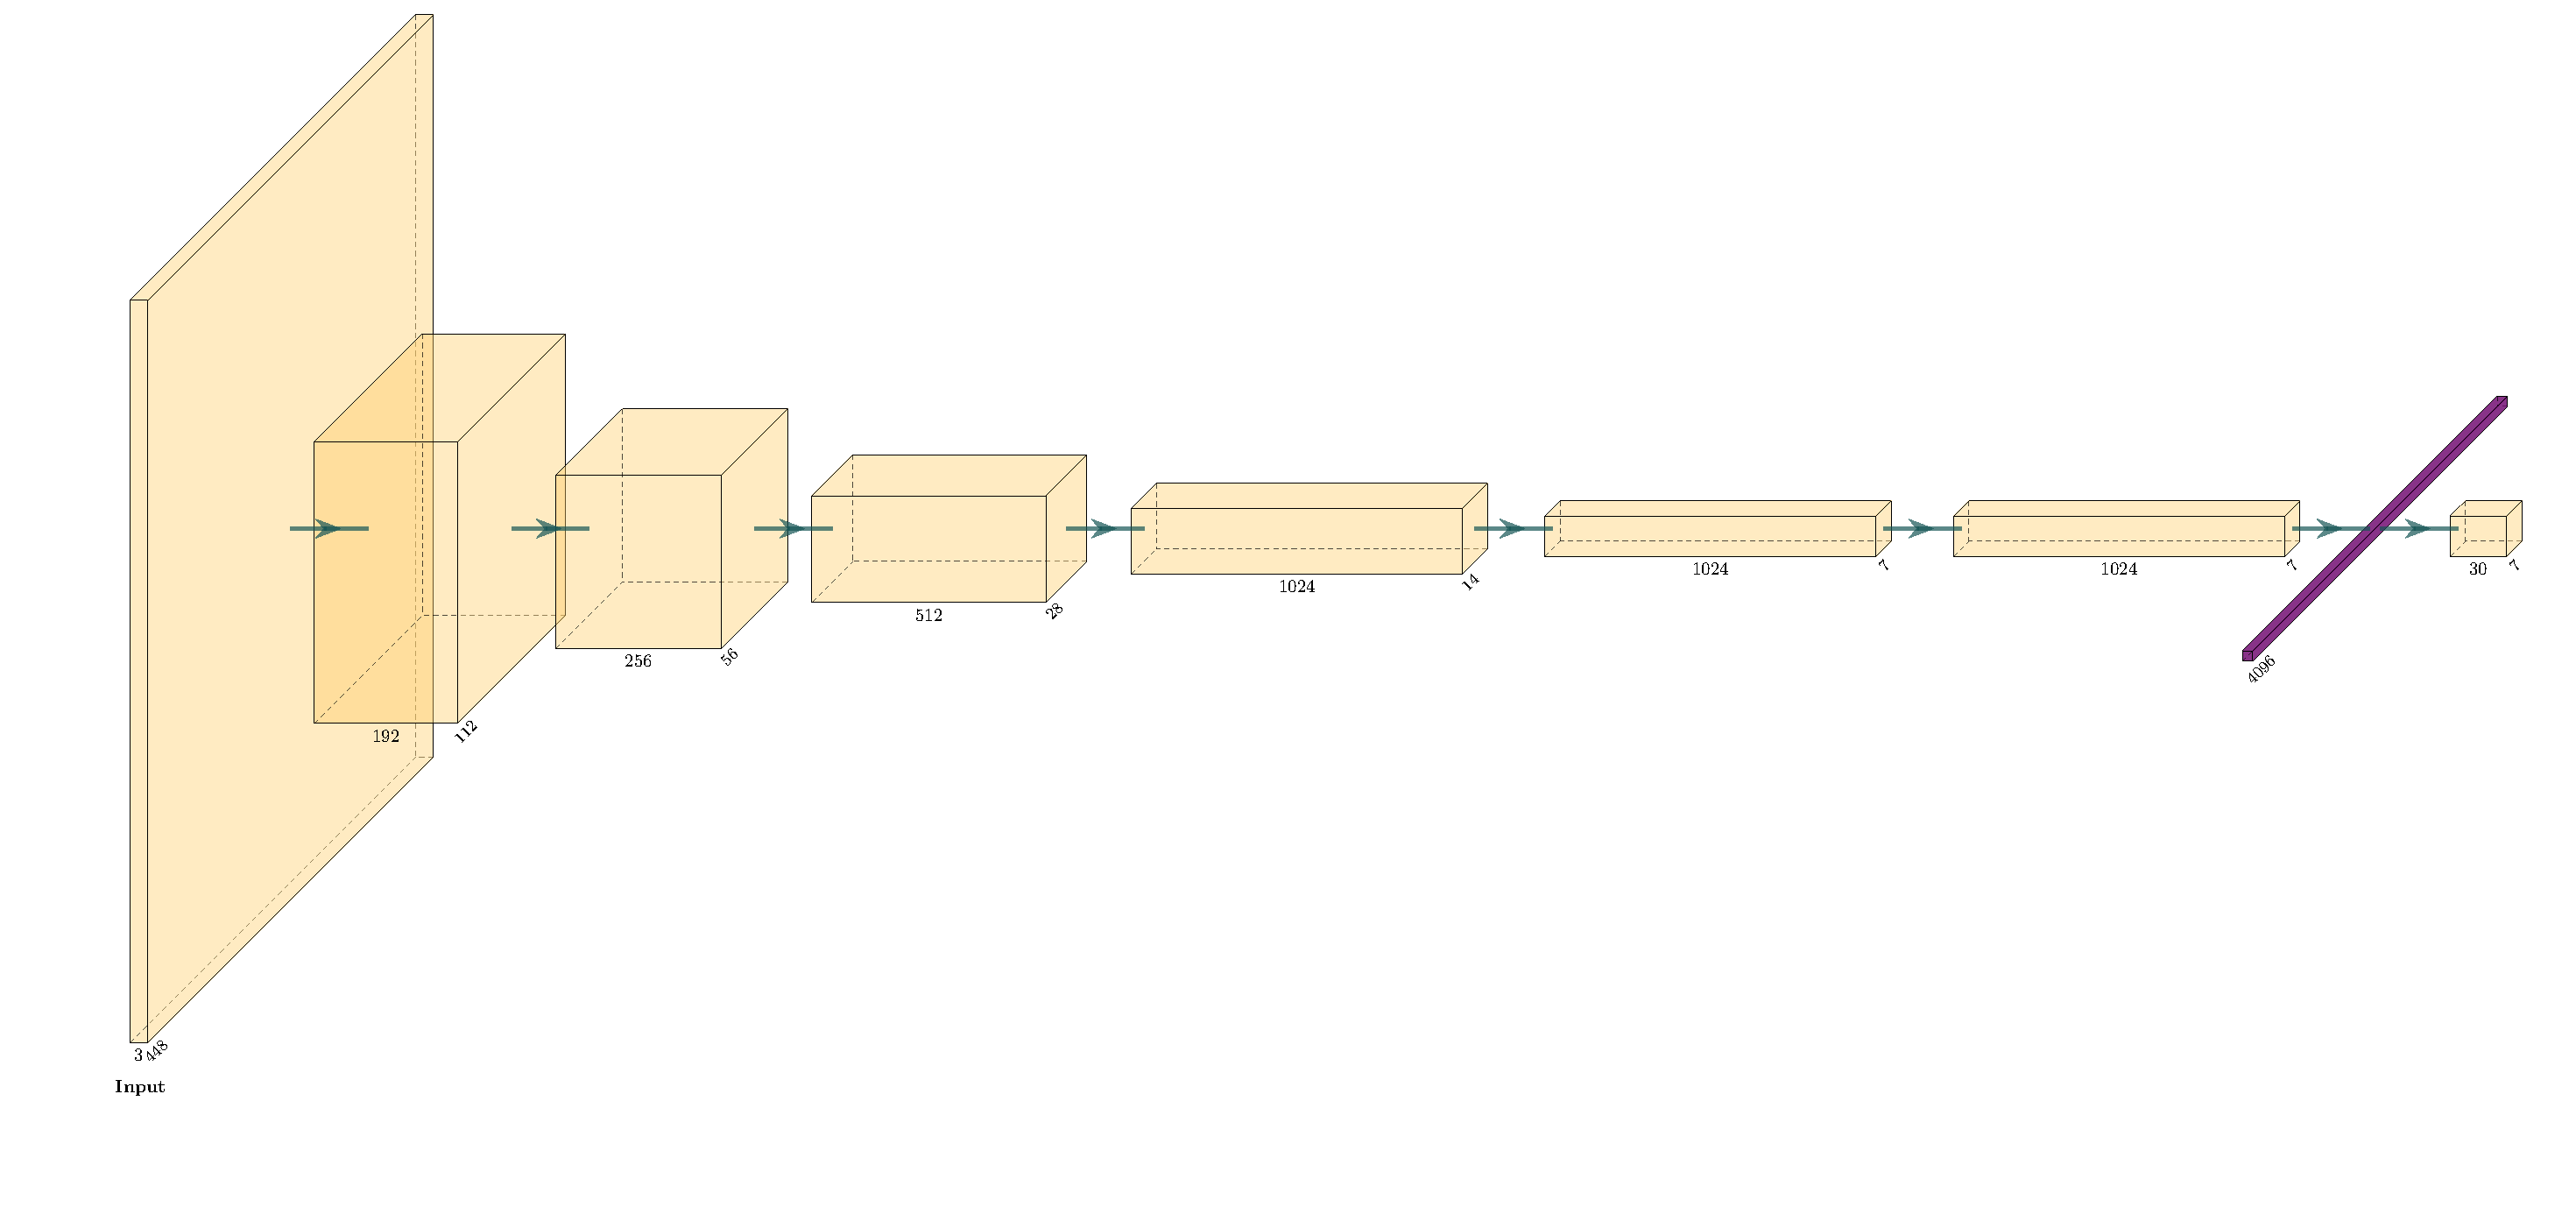
\includegraphics[width=\textwidth]{image/yolo}
  \label{fig:yolo}
\end{figure}

\ac{YOLO}v2 or \ac{YOLO}9000 improves on \ac{YOLO} with the introduction of anchor boxes, allowing the network to detect objects in regions of the image instead of the whole image at once \cite{redmon2017yolo9000}. Furthermore, all fully connected layers are removed from the \ac{YOLO}v2 network architecture and the output of one of the earlier layers is passed through and concatenated into one of the last layers as seen in \figureref{fig:yolov2}. The first 23 layers of the network, or 6 boxes in the figure, are also referred to as the Darknet19 backbone, while the last 4 layers are the detection head. \ac{YOLO}v2 also introduced batch normalization, a better loss function and multi-scale training, which refers to its ability to adapt its network size to different input image sizes from $320 \times 320$ to $608 \times 608$ pixels.

\begin{figure}
  \caption{Visualization of the most important layers of the \ac{YOLO}v2 network. Here, the tensor width and height are mapped by $x \mapsto x^{0.7}$ and tensor length, eg. the feature map length, is scaled by $x \mapsto x^{0.5}$. It was created using \href{https://github.com/jnccd/PlotNeuralNet}{a modified version of the PlotNeuralNet tool} \cite{haris_iqbal_2018_2526396}.}
  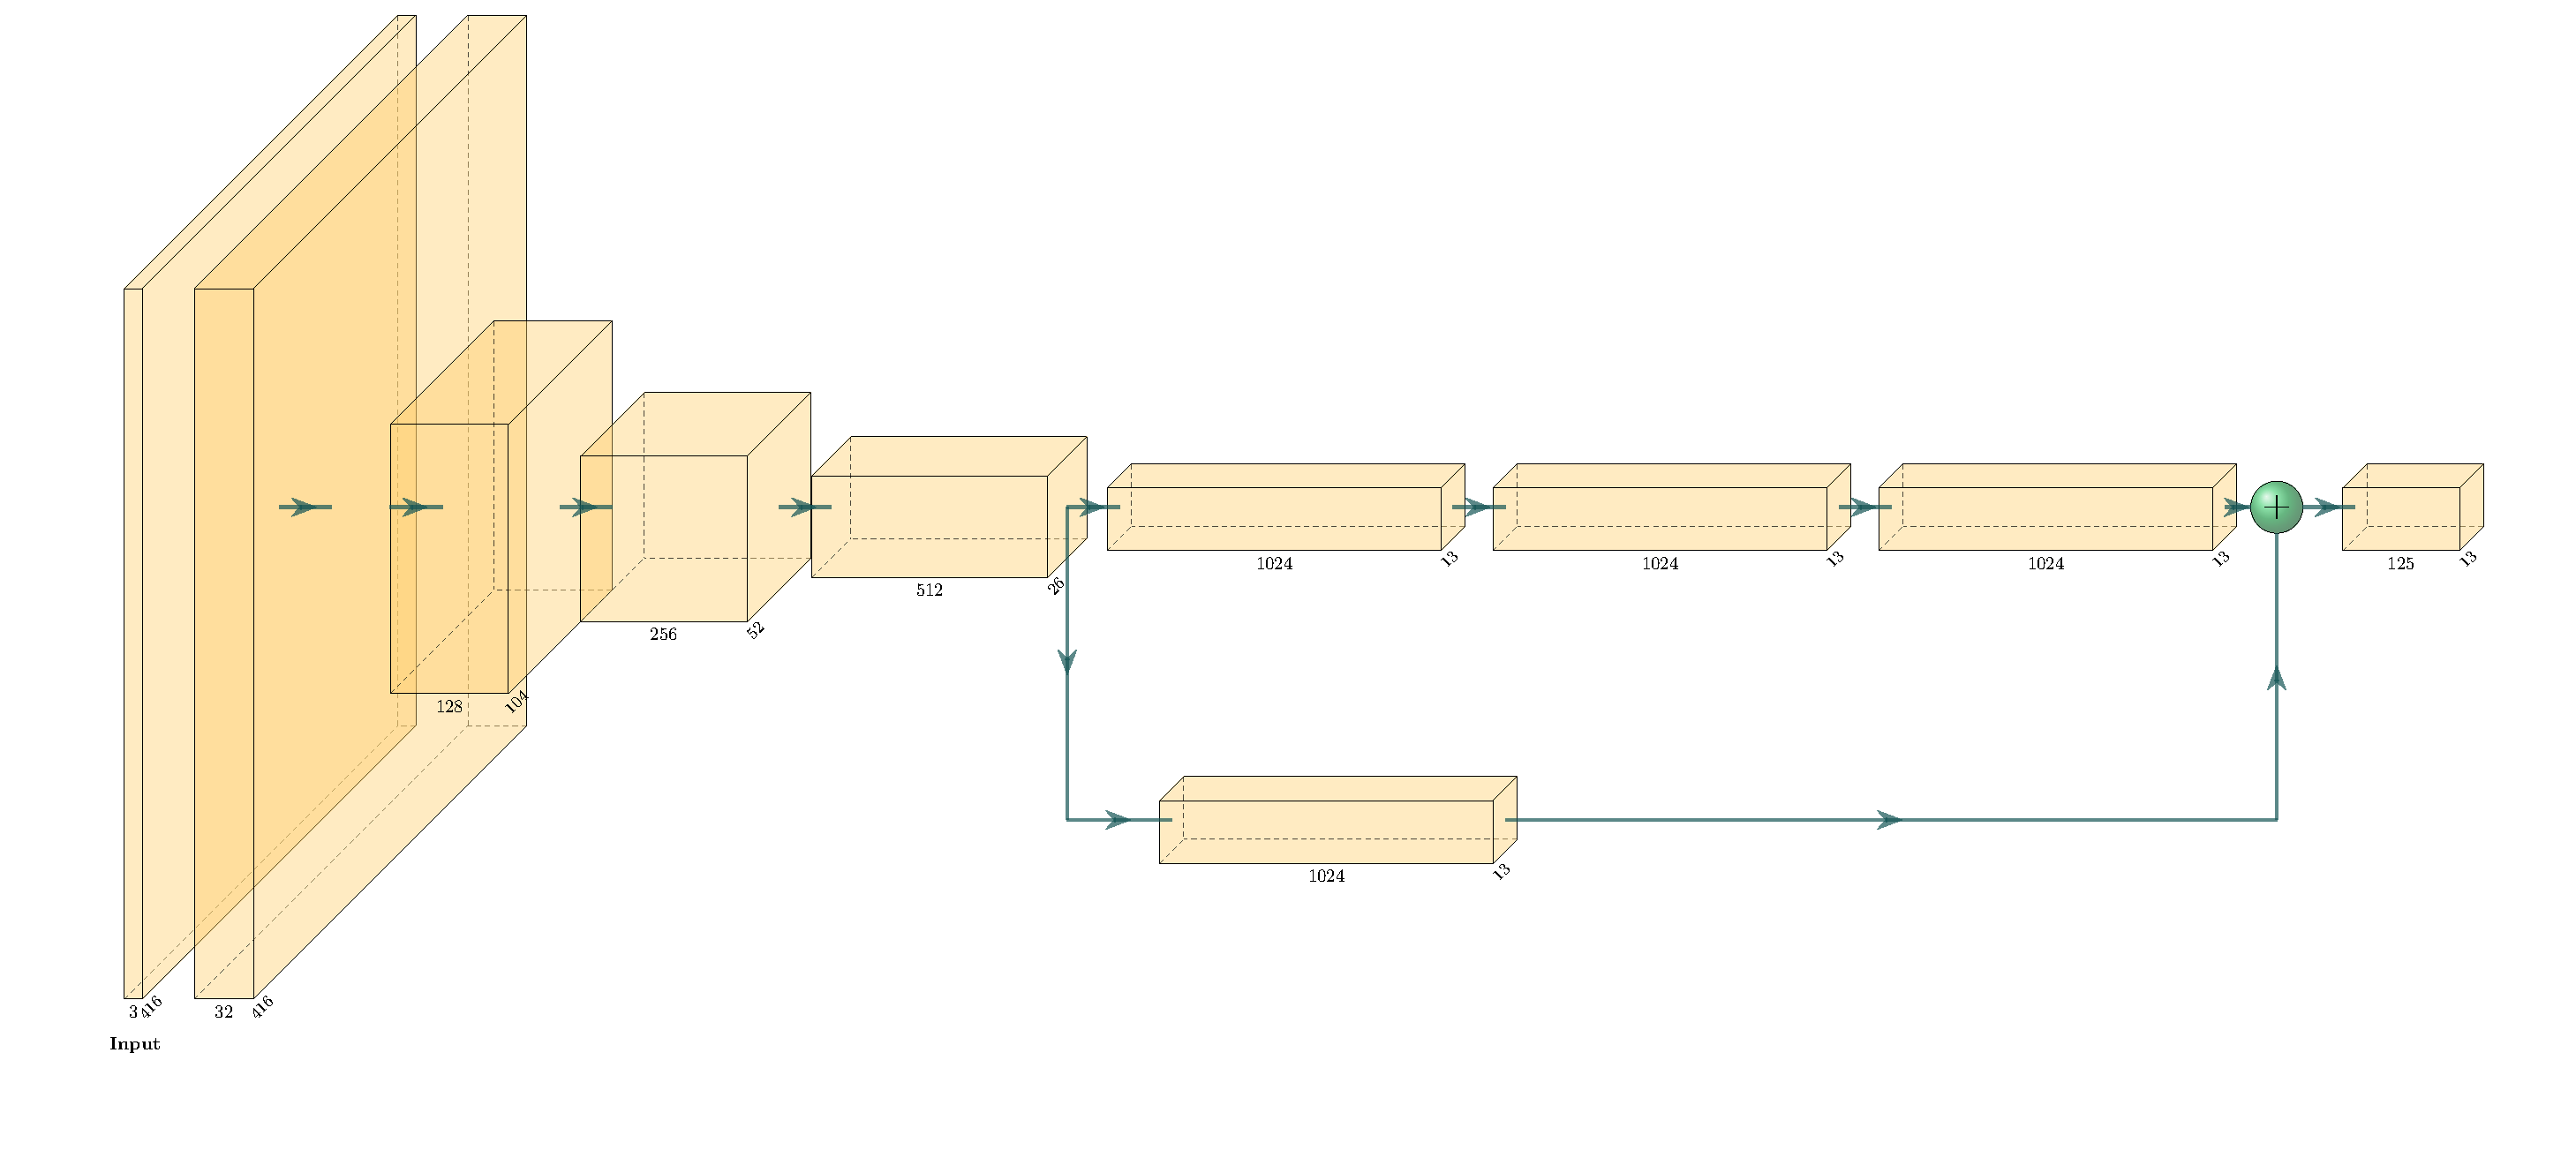
\includegraphics[width=\textwidth]{image/yolov2}
  \label{fig:yolov2}
\end{figure}

\ac{YOLO}v3 mainly improves the network architecture by developing approaches from \ac{YOLO}v2 and Darknet-19 further to create the Darknet-53 backbone, which got its name from the 53 convolutional layers it contains \cite{redmon2018yolov3}. \ac{YOLO}v3 also introduced a more efficient loss function and \ac{SPP}, which allowed it to detect bounding boxes at different scales more effectively \cite{jani2023model}. % TODO: Describe head?

\section{Later YOLO Versions}

\begin{figure}
  \caption{Timeline showing different \ac{YOLO} versions over time which is based on the timeline from Terven et al. \cite{terven2023comprehensive}.}
  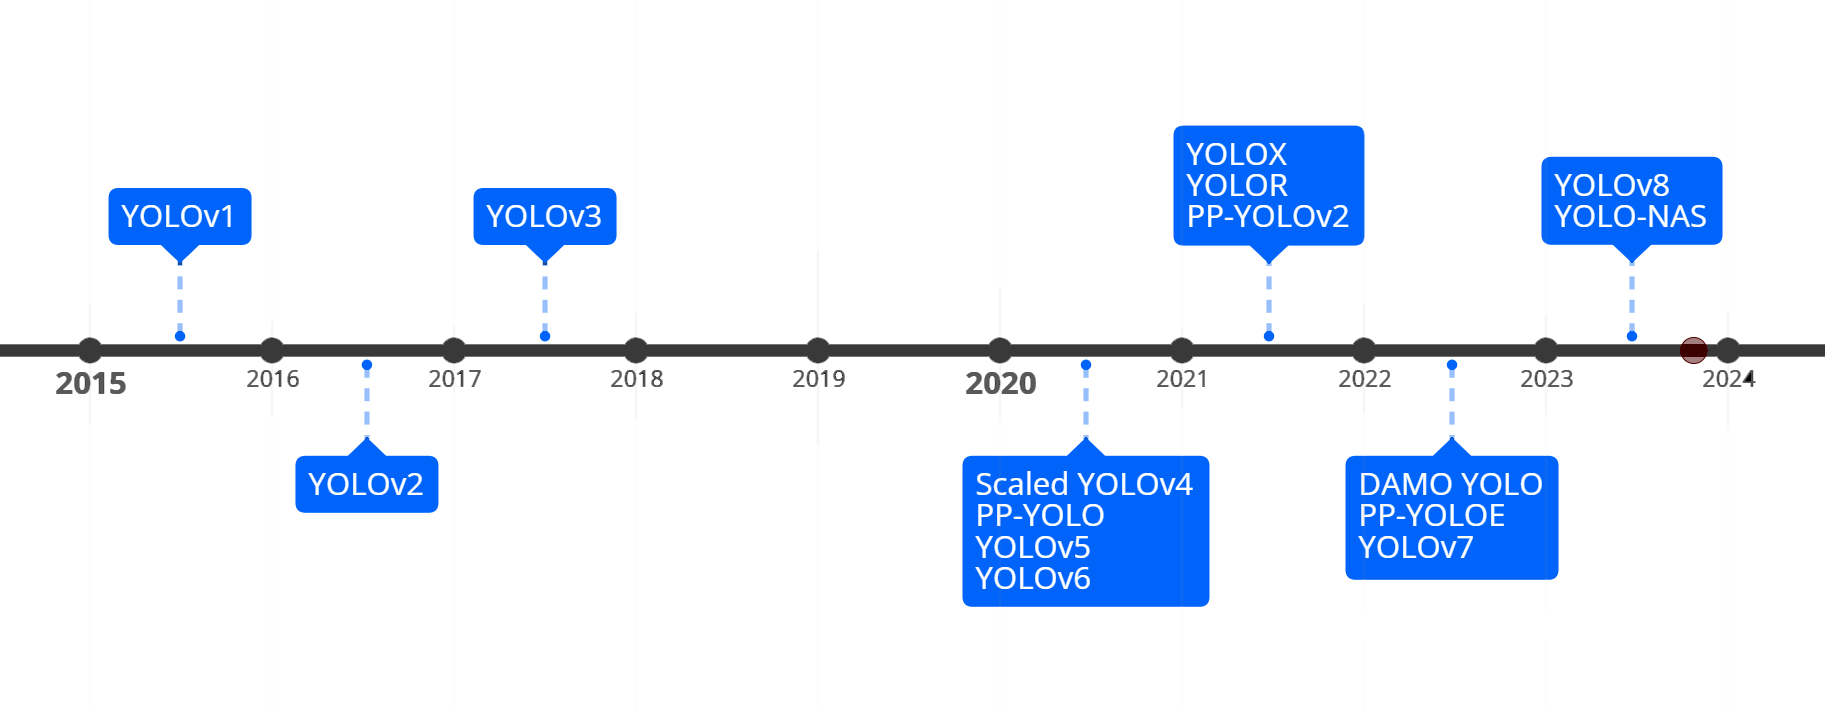
\includegraphics[width=\textwidth]{image/timeline_fix}
  \label{fig:yolo_timeline}
\end{figure}

While the first three \ac{YOLO} versions were developed by the same developers, starting with \ac{YOLO}v4, various developers started releasing \ac{YOLO} versions. A full timeline of the releases can be seen in \figureref{fig:yolo_timeline}. 

Based on the comparison of \ac{mAP} scores from Terven et al. \cite{terven2023comprehensive}, the three best \ac{YOLO} models on the \ac{COCO} challenge are \ac{YOLO}v7, Scaled-\ac{YOLO}v4 and \ac{YOLO}v5. 
Since the model should be used on a smartphone, only the smaller versions of the models are relevant. Wang et al. showed that \ac{YOLO}v7-tiny depending on the metric outperforms or is similar to \ac{YOLO}v4-tiny \cite{wang2023yolov7}. 
Unlike the other two considered \ac{YOLO} versions, \ac{YOLO}v5 provides multiple versions like \ac{YOLO}v5s and \ac{YOLO}v5m in between teh sizes tiny and large. 
The larger \ac{YOLO}v5m is still recommended for modern smart phones\footnote{\url{https://docs.ultralytics.com/yolov5/tutorials/tips\_for\_best\_training\_results}, accessed on 04.12.2023}. 
However, since the smaller \ac{YOLO}v5s likely has support on more devices with smaller memory and since \ac{YOLO}v5s is the \ac{YOLO}v5 model closest to \ac{YOLO}v7-tiny in parameter count, I chose to focus on it. %Similarly to the first comparison, 
The \ac{mAP} scores of \ac{YOLO}v5s are comparable to \ac{YOLO}v7-tiny, with \ac{YOLO}v7-tiny having a moderately higher \ac{COCO} 50-95 \ac{mAP} score and \ac{YOLO}v5s having a slightly higher \ac{COCO} 50 \ac{mAP} score\footnote{\url{https://pytorch.org/hub/ultralytics_yolov5/}, accessed on 04.12.2023} \cite{wang2023yolov7}. 
Finally, I chose to use \ac{YOLO}v5s due to the clear documentation and popularity of \ac{YOLO}v5, as seen in the number of github stars\footnote{\url{https://github.com/AlexeyAB/darknet}, accessed on 04.12.2023}\footnote{\url{https://github.com/ultralytics/yolov5}, accessed on 04.12.2023}\footnote{\url{https://github.com/WongKinYiu/yolov7}, accessed on 04.12.2023}. Furthermore, I implemented \ac{YOLO}v8 and \ac{YOLO}-NAS due to their recency and \ac{YOLO}v8's similarity to \ac{YOLO}v5.

% However, \ac{YOLO}v7 only provides models in sizes \ac{YOLO}v7-tiny, \ac{YOLO}v7, \ac{YOLO}v7-X and larger variations \cite{wang2023yolov7}. While \ac{YOLO}v7-tiny may be promising for older devices with its 6.2 million parameters, \ac{YOLO}v5s only has about 1 million parameters more, still fits on modern smart phones, and outperforms \ac{YOLO}v7-tiny on the \ac{COCO} challenges 50 \ac{mAP} score\footnote{\url{https://pytorch.org/hub/ultralytics_yolov5/}, accessed on 04.12.2023}. However, the next larger model called \ac{YOLO}v7 is too large for usage on current smart phones with its 36.9 million parameters. The larger versions of \ac{YOLO}v7 are still likely a good choice for a cloud based detection due to their effectiveness. Scaled-\ac{YOLO}v4 similarly does not provide model sizes between  Furthermore, the \ac{mAP} difference 
% For this work, I will focus on \ac{YOLO}v5, due to its popularity and therefore its good documentation.  \ac{YOLO}v8 and \ac{YOLO}-NAS due to their recency and \ac{YOLO}v8's similarity to \ac{YOLO}v5.

\section{YOLOv5}

%instead of the developers of the first three \ac{YOLO} versions
\ac{YOLO}v5 was developed by Ultralytics and introduces small changes to the architecture, new box coordinates, a build target process as well as new augmentation techniques\footnote{\url{https://docs.ultralytics.com/yolov5/tutorials/architecture_description}, accessed on 20.10.2023} \cite{gjocher2022yolov5,terven2023comprehensive}. \ac{YOLO}v5 also made hyperparameter optimization easier and added quality of life features. \ac{YOLO}v5 provides models in five different sizes: \ac{YOLO}v5n (nano), \ac{YOLO}v5s (small), \ac{YOLO}v5m (medium), \ac{YOLO}v5l (large), and \ac{YOLO}v5x (extra large).

\subsection{Architecture}

\ac{YOLO}v5's network architecture consists of a backbone, a neck and a head, which are connected to each other in that order \cite{jani2023model}. \ac{YOLO}v5's backbone is the CSP-Darknet53 structure, which was the structure that \ac{YOLO}v4 used \cite{bochkovskiy2020yolov4}. \ac{YOLO}v5's Neck consists of the \ac{SPPF}, which is a more efficient version of \ac{YOLO}v3's \ac{SPP}, and new \ac{CSP-PAN} structures, which improve the information flow through the network \cite{liu2018path}. \ac{YOLO}v5 uses the same head structure as \ac{YOLO}v3 at the end of the network. The entirety of the network is visualized in \figureref{fig:yolov5}.

\begin{figure}
  \caption{Visualization of the most important layers and blocks of the entire \ac{YOLO}v5 network. Here, the tensor width and height being mapped by $x \mapsto x^{0.7}$ and tensor length, eg. the feature map length, being scaled by $x \mapsto x^{0.5}$. The head structure of the \ac{YOLO}v5 network was simplified to a single tensor for this figure. The visualization was created using \href{https://github.com/jnccd/PlotNeuralNet}{a modified version of the PlotNeuralNet tool} \cite{haris_iqbal_2018_2526396}.}
  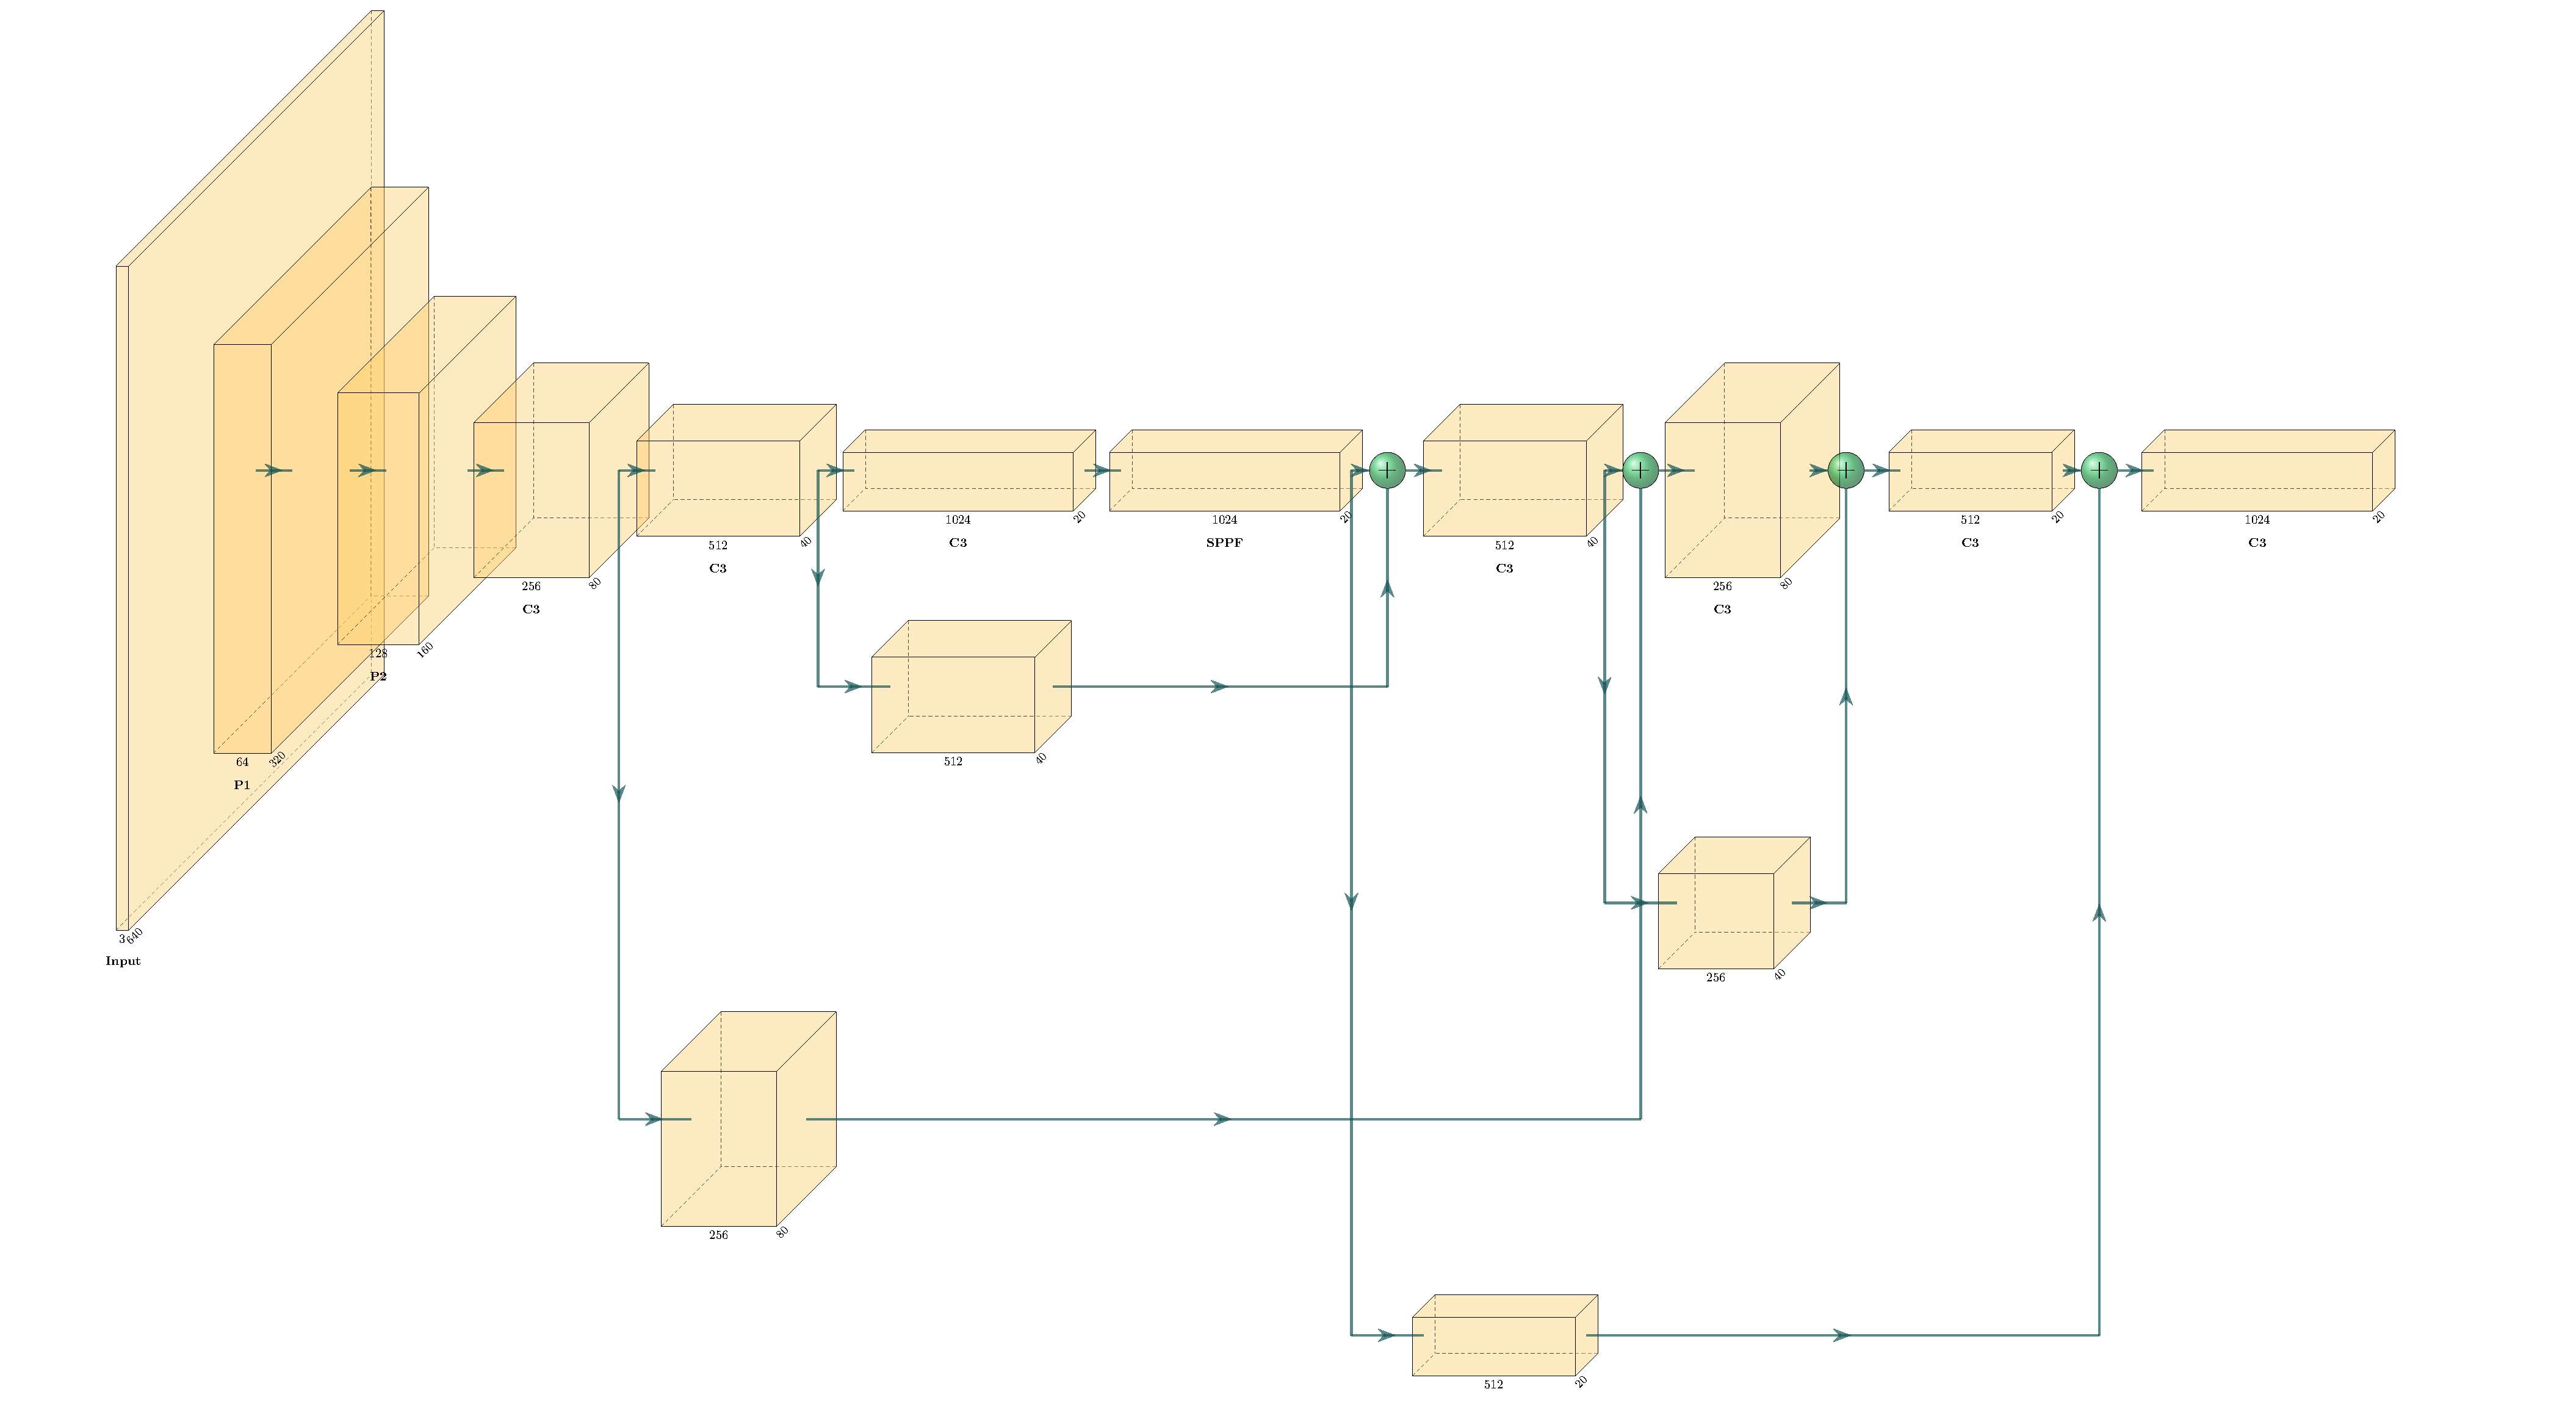
\includegraphics[width=\textwidth]{image/yolov5}
  \label{fig:yolov5}
\end{figure}

\subsection{Built-in Data Augmentation}

\ac{YOLO}v5 also comes with predefined augmentation techniques. 

\begin{itemize}
  \item Mosaic Augmentation: This technique places four training images next to each other in one bigger image.
  \item Random Affine Transformations: This technique applies random rotation, scaling, translation, and shearing to the image.
  \item HSV Augmentation: This technique applies random changes to the Hue, Saturation, and Value of pixels within a certain range for each of the values.
  \item Random Horizontal Flip: This technique randomly flips the image around the y axis.
\end{itemize}

\ac{YOLO}v5 further defines augmentations such as Copy-Paste Augmentation and MixUp Augmentation. However, these augmentations were disabled by default and not used over the course of this thesis.

\section{YOLOv8}

\ac{YOLO}v8 is the second \ac{YOLO} version from Ultralytics and provides multiple models in the same sizes as \ac{YOLO}v5\footnote{\url{https://docs.ultralytics.com/models/yolov8/}, accessed on 24.10.2023} \cite{terven2023comprehensive}. \ac{YOLO}v8 is anchor-free, which simplifies the training and decoding process. For the bounding box loss \ac{YOLO}v8 uses \ac{CIoU} \cite{zheng2020distance}, which besides the overlap area is also based on the central point distance and aspect ratio of the bounding boxes, as well as \ac{DFL} \cite{li2020generalized}. %\ac{YOLO}v8 also provides a segmentation model.

\section{YOLO-NAS}

\ac{YOLO}-NAS was developed by Deci which develops production grade models \cite{terven2023comprehensive}. The architecture of \ac{YOLO}-NAS was found by Deci's proprietary \ac{NAS} technology AutoNAC and comes in three sizes: \ac{YOLO}-NAS-S, \ac{YOLO}-NAS-M and \ac{YOLO}-NAS-L. The \ac{YOLO}-NAS models were pre-trained on the Objects365 dataset, which is newer and larger than the \ac{COCO} dataset and gets its name from its 365 object categories \cite{shao2019objects365}. Afterwards, they were trained on the \ac{COCO} dataset.

% TODO?: \section{MobileNetV2}

\section{ViTs}

After the application of transformer blocks in natural language processing was successful, they were also introduced into other domains, such as visual processing, resulting in \acp{ViT}. The application of transformers on vision tasks works by slicing the input image into many patches \cite{dosovitskiy2020image}. The pixel data of these patches is further divided and interpreted as word vectors. These "visual words" can then be fed into a transformer based network.

\acp{ViT} mark the newest major change in network architecture for the object detection task. The advantage of \acp{ViT} is their scalability, making \cite[models of unprecedented size]{dosovitskiy2020image} trainable. However, in this work I aim to develop a detection system that would preferably run directly on patients smart phones, which makes large models impractical. Furthermore, development on ConvNeXt showed that, when trained using similar modern training techniques, large convolutional networks can perform similarly well or better than vision transformers. Therefore, the improvements may not stem from network architecture itself \cite{liu2022convnet}.

\section{U-Net}

\begin{figure}
  \caption{Visualization of a U-Net which was taken from the examples of the \href{https://github.com/HarisIqbal88/PlotNeuralNet}{PlotNeuralNet tool} \cite{haris_iqbal_2018_2526396}.}
  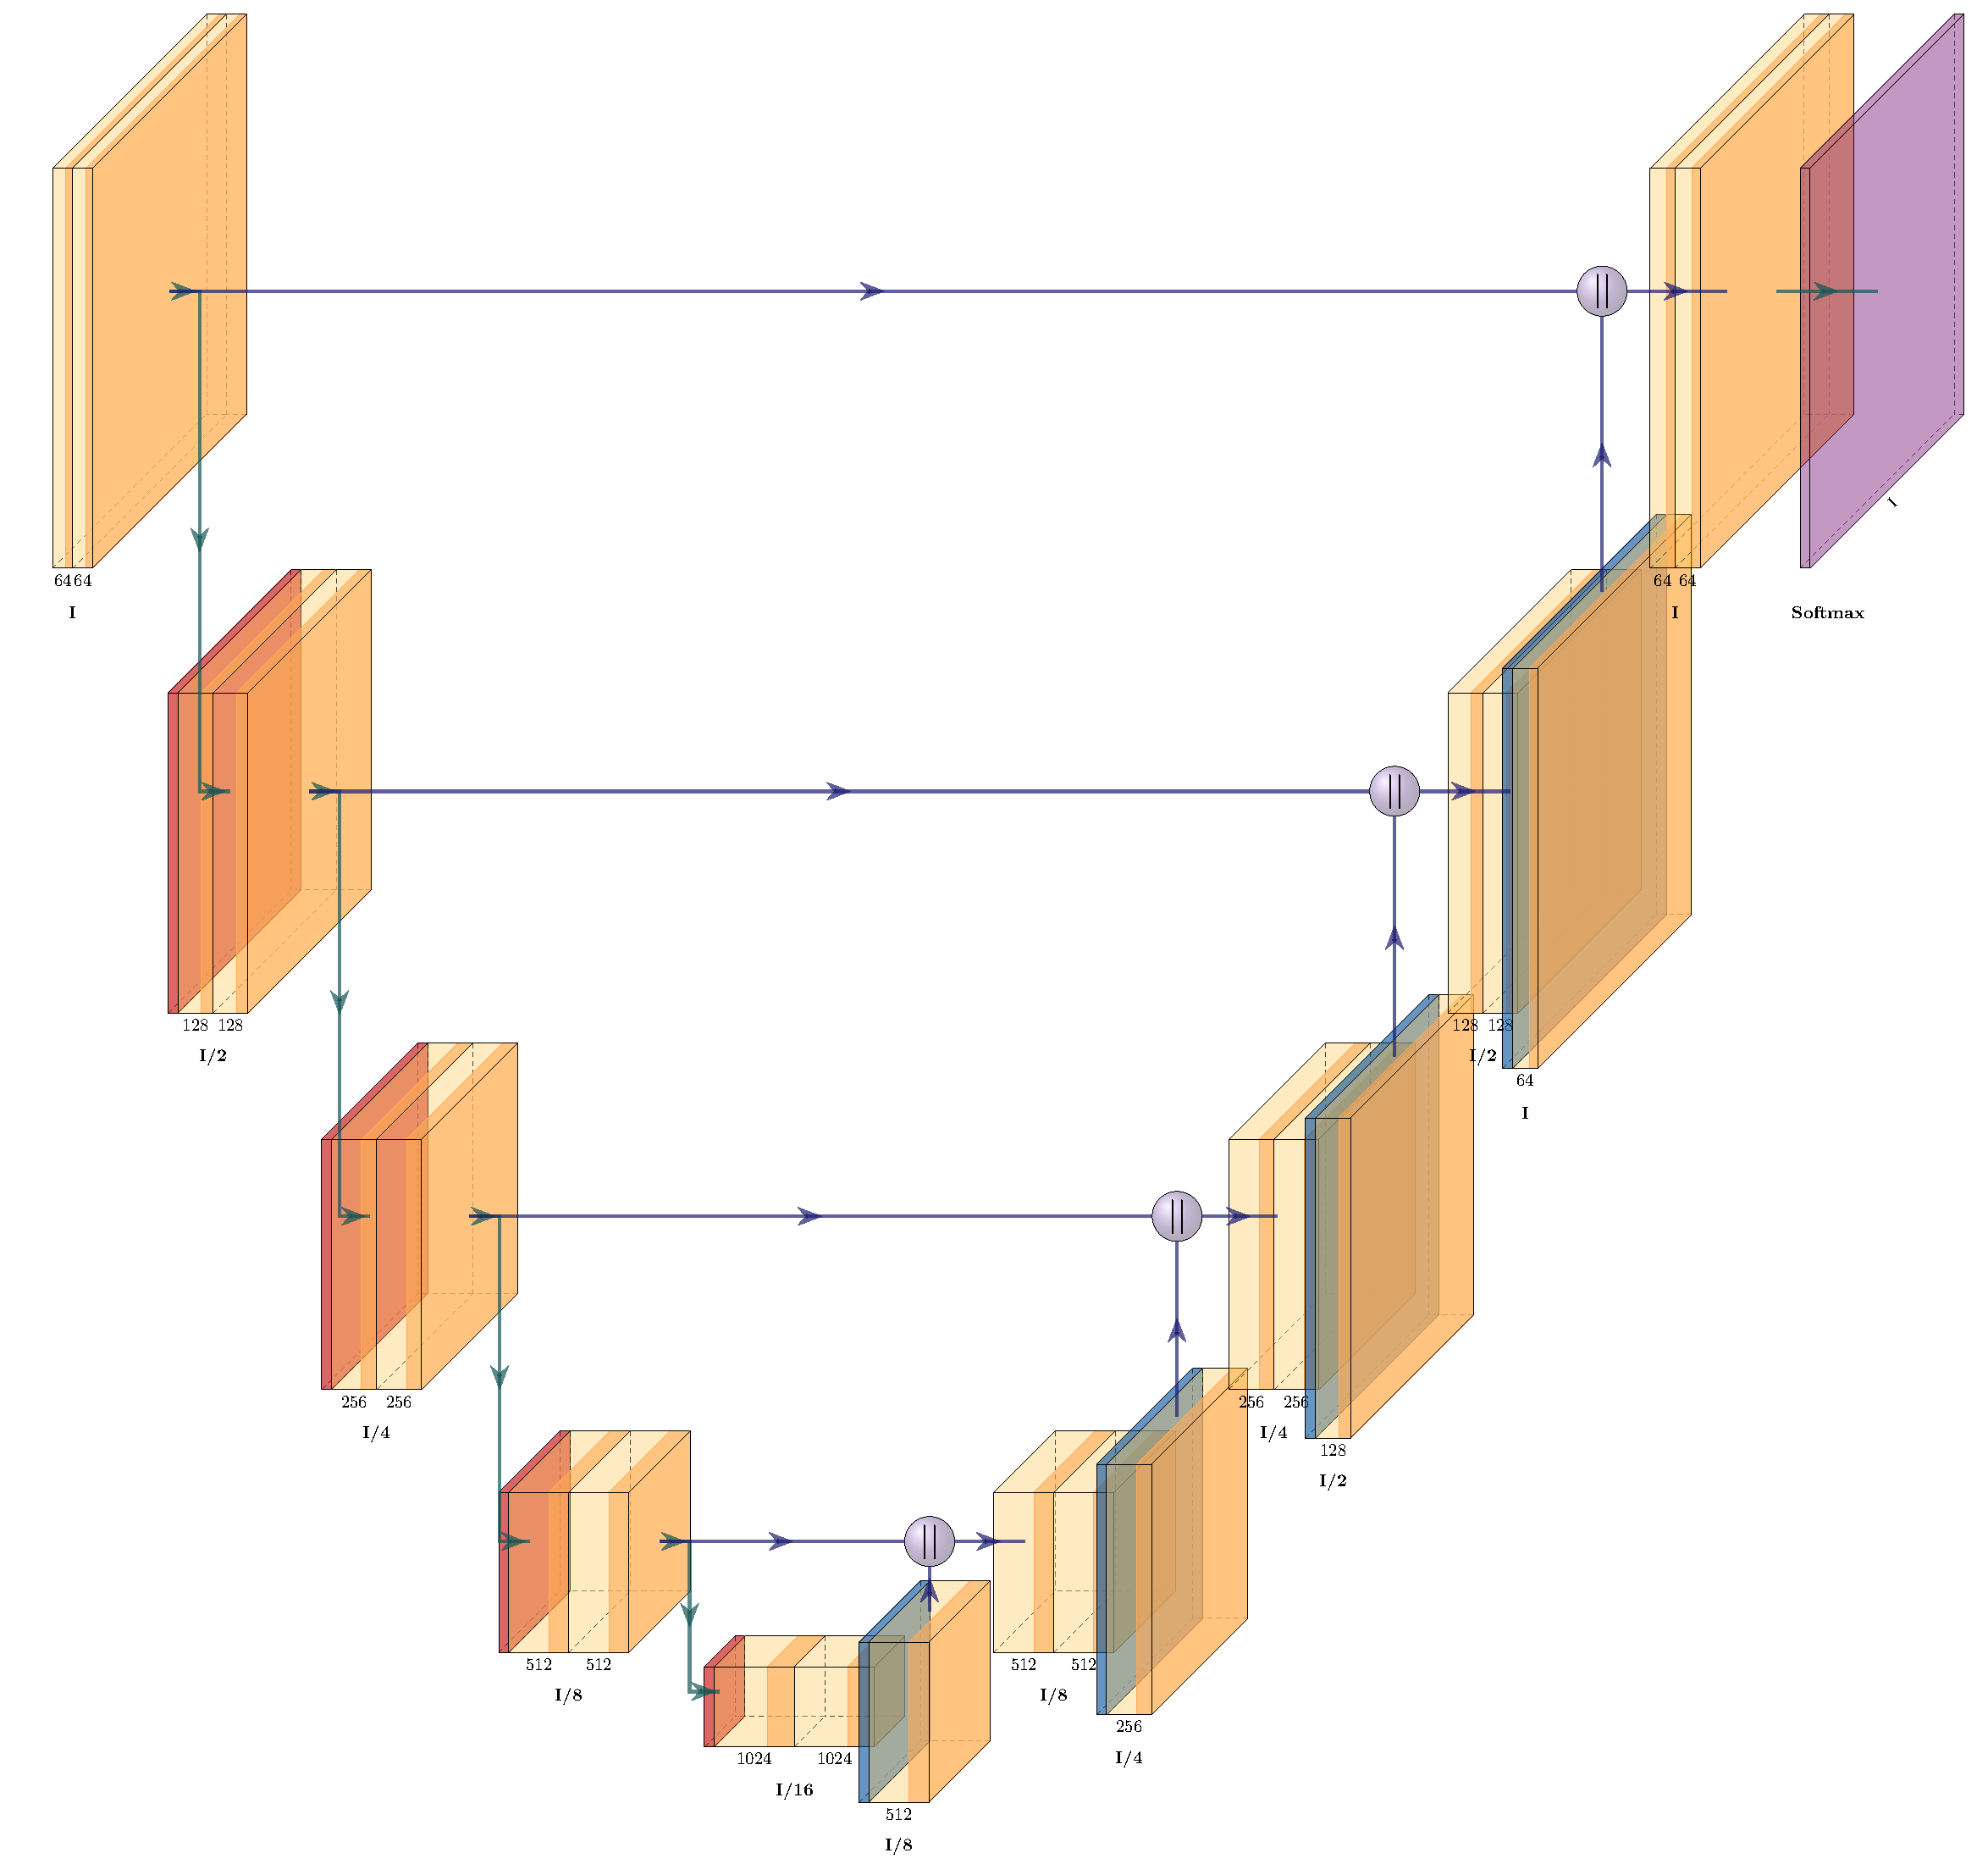
\includegraphics[width=0.8\textwidth]{image/Unet_ushape}
  \label{fig:unet}
\end{figure}

An U-Net is a \ac{CNN} that was developed for biomedical image segmentation \cite{DBLP:journals/corr/RonnebergerFB15}. Its architecture is based on the fully convolutional network proposed by Long et al. \cite{DBLP:journals/corr/LongSD14} and extends the contracting network by following upsampling layers. Visualizing the layers such that their y position is based on the amount of feature maps they output yields the characteristic u-shape for the network, as seen in \figureref{fig:unet}. Furthermore, it uses feature channels to propagate context information from earlier layers to provide the upsampling path with missing information which may be lost during the contracting layers. This missing information can then help in generating high resolution segmentation masks.

\chapter{Methodology and Implementation}
\label{chap:implement}

In this chapter I describe how I structured my code and why, as well as the core ideas of some algorithms. Furthermore, I describe the hardware that was used for training.

% \section{Goals}

% % TOxDO: Talk about the whole image and pet parts of the inference pipeline here

% My goal for the implementation is to write a software framework that allows me to train the custom data given to me on a wide variety of object detection \acp{NN} using a wide variety of training techniques and to evaluate the effectiveness of all those approaches.

% Furthermore, I want to develop a second part of the pipeline which uses the areas of interest detected by the object detection models for the detection of the marker corners.

\section{Development Environment}

Most training for this work was done on the 'lena' server of the \ac{MIP} working group of the Kiel University. This server contains 128GB RAM and eight Nvidia GeForce RTX 2080Ti \acp{GPU} with 12GB VRAM each. Local training was done on a computer with 32GB RAM and a Nvidia GeForce RTX 3060Ti \ac{GPU} with 8GB VRAM.

Training on the server was done using a Docker Image and locally it was done in a conda environment. During development I used both TensorFlow and PyTorch, so for simplicity I chose to install them both in the same environments. This is possible because both the PyTorch version 2.0.1 and the TensorFlow version 2.12 depend on the same CUDA Toolkit version 11.8 as well as on the cuDNN version 8.4.1.50. % TODO: Dont use ac here? I only use CUDA, cuDNN once 

\section{Classic Approaches}

To validate that a neural network based approach is necessary in this case, I tested some approaches using algorithms from \ac{OpenCV}, which do not require machine learning. For these tests, I chose a test image from the given data, on which the markers were facing the camera and had as much visible contours as possible, which can be seen in \figureref{fig:classic_base_img}. 

\begin{figure}
  \caption{Test Image for Classic Approaches.}
  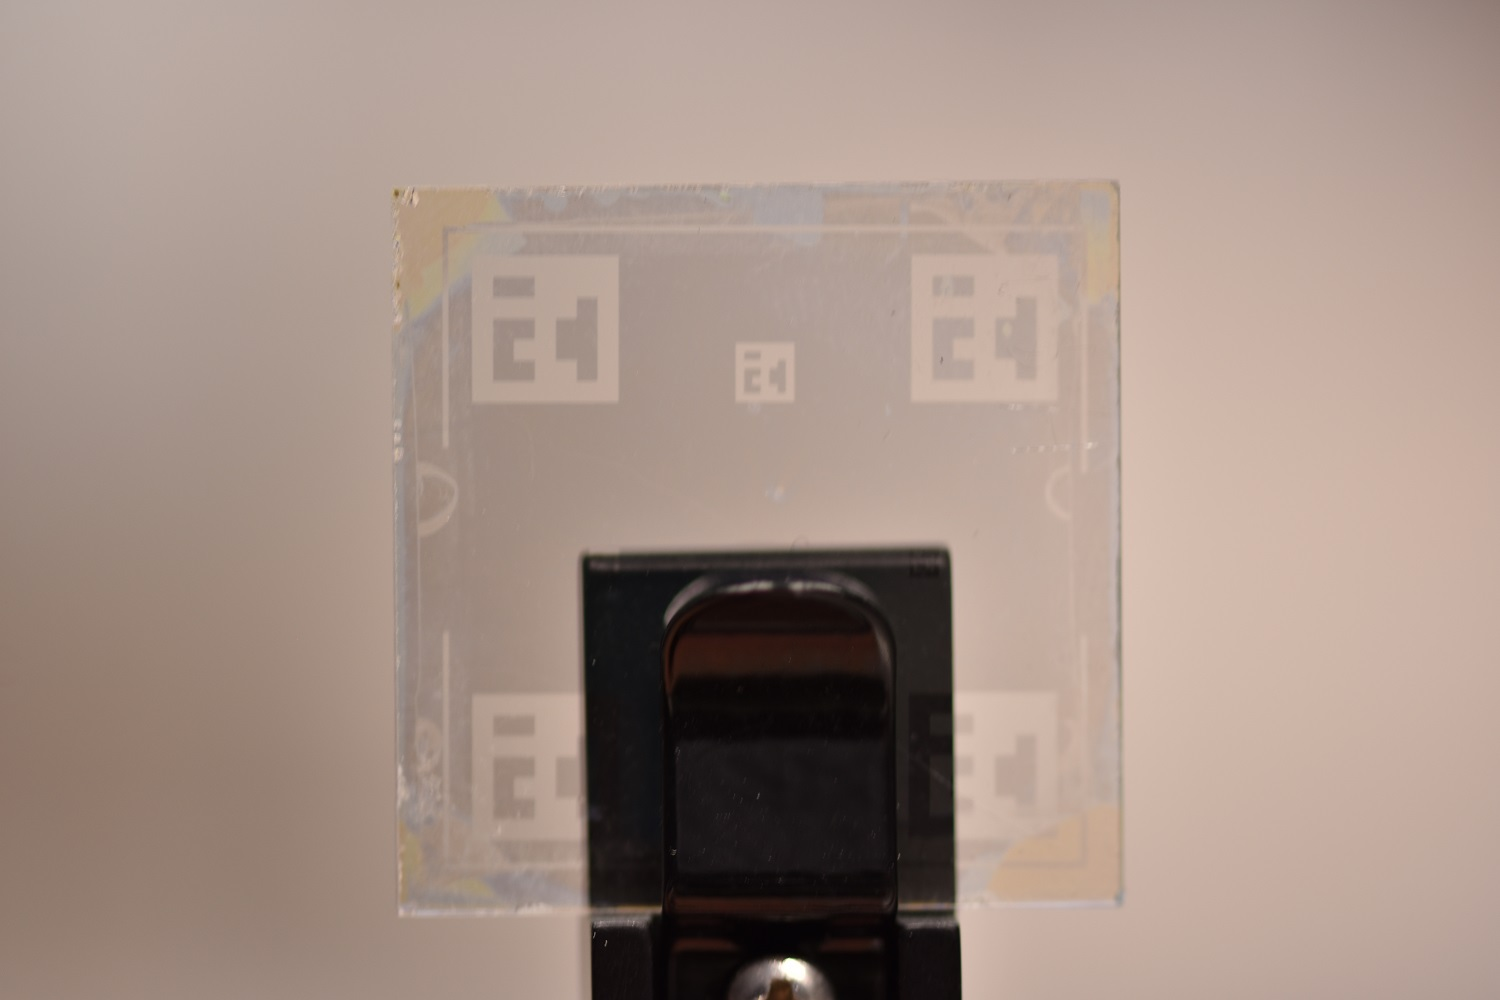
\includegraphics[width=0.6\textwidth]{image/classic_base_img}
  \label{fig:classic_base_img}
\end{figure}

\subsection{Open CV ArUco Detection}

\begin{figure}
  \centering
  \subcaptionbox{Canny edge output}
     {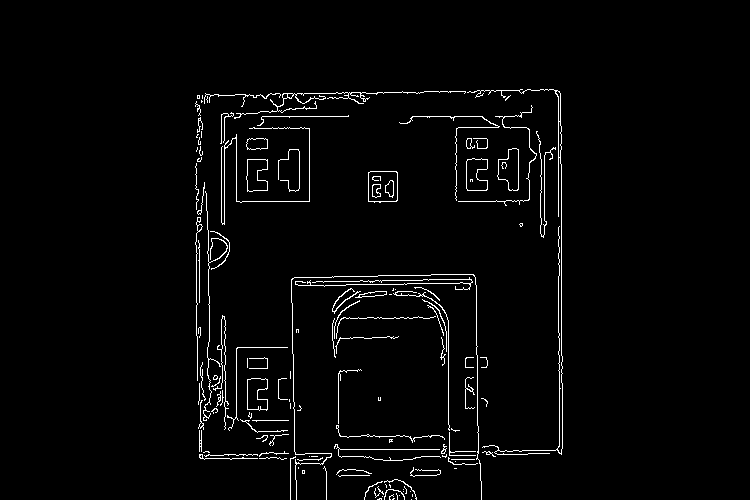
\includegraphics[width=0.4\textwidth]{image/classic_base_img_opencv_det_edges}}
  \subcaptionbox{Suzuki and Abe algorithm output}
     {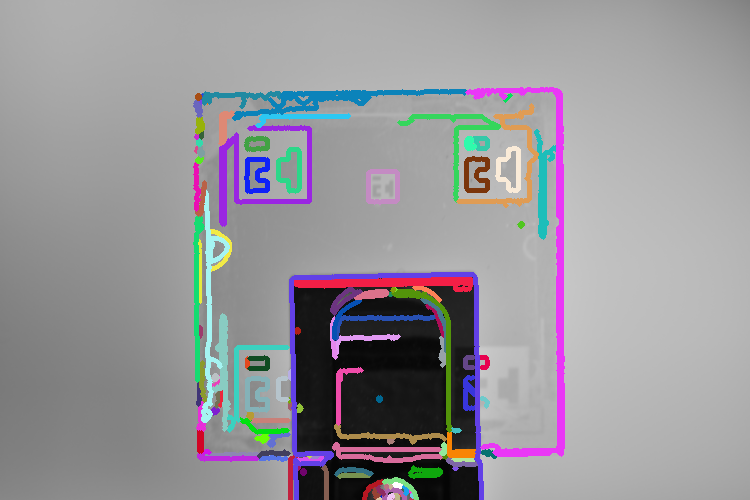
\includegraphics[width=0.4\textwidth]{image/classic_base_img_opencv_det_contours}}
  \caption{First steps of the \ac{OpenCV} \ac{ArUco} detection pipeline. Polygons are randomly colored to make them distinguishable.}
  \label{fig:classic_base_img_opencv}
\end{figure}

The built-in \ac{OpenCV} \ac{ArUco} detector does not detect any markers in the chosen base image. To find out why, I roughly recreated the first steps of the \ac{ArUco} detector using \acp{OpenCV} built-in algorithm implementations. The recreated pipeline mainly consists of the canny edge detector and the \texttt{findContours} and \texttt{approxPolyDP} methods applied to each level of an image pyramid. 

The broken contours of the \ac{ArUco} marker edges seen in \figurereft{fig:classic_base_img_opencv}{(a)} skewed the results of the polygon contour detection of the Suzuki and Abe algorithm seen in \figurereft{fig:classic_base_img_opencv}{(b)}. That the \ac{ArUco} detector from \ac{OpenCV} has no further handling for this case explains why the \ac{ArUco} markers on photonic crystals could not be detected, as well as the findings in \autoref{sec:aruco_det}.

% When filtering for only polygons with four vertices, the small polygon is detected on one scale, as seen on \figurereft{fig:classic_base_img_opencv}{(a)}. The better detection accuracy here may be due to cherry picked algorithm parameters. Without the filter in \figurereft{fig:classic_base_img_opencv}{(b)}, the problems of the polygon detection become apparent since the algorithm does not work well with broken contours, which may in part explain the findings in \autoref{sec:aruco_det}.

\subsection{Histogram}

The idea of the histogram approach is that the pixel gradient histogram distributions in a window around the marker in the image should have a similar distribution on each of the markers due to the structure of the \ac{ArUco} marker in the image.

\begin{figure}
  \centering
  \subcaptionbox{Output of Histogram Difference, with the top left marker being the histogram baseline}
     {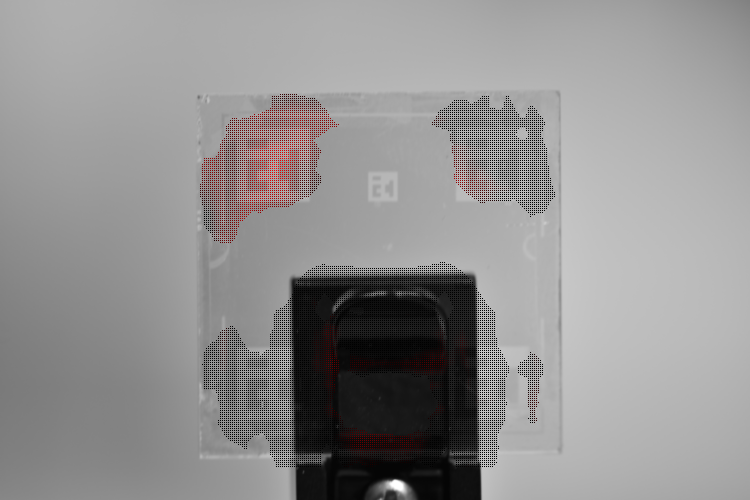
\includegraphics[width=0.4\textwidth]{image/classic_hist_markerynesses}}
  \subcaptionbox{Output of Histogram Peak based Score}
     {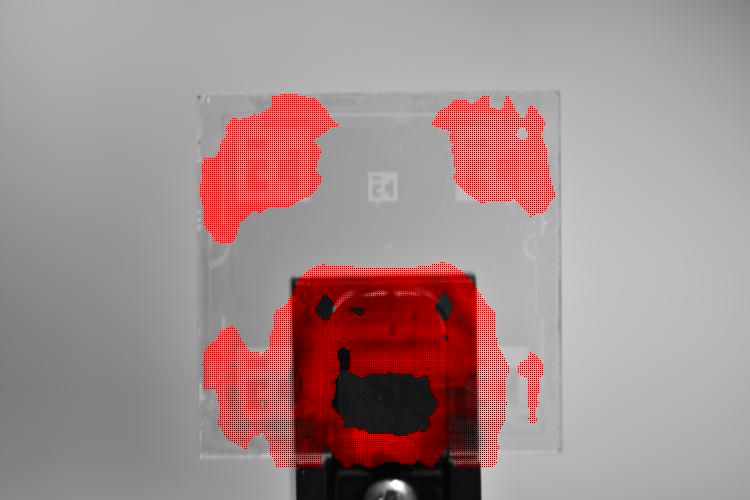
\includegraphics[width=0.4\textwidth]{image/classic_markeryness}}
  \caption{Output of the Histogram based Approach in which the pixels of middle points of all windows that passed the candidate check are repainted. The redness of the repainted pixel represents the score of its window.}
  \label{fig:markeryness_scores}
\end{figure}

For this approach, the image is firstly scaled in an image pyramid. For each entry in the image pyramid, a thresholded version is computed using adaptive thresholding, as well as the image gradients in x and y direction and polar coordinate versions of the gradients. Afterwards, the image is traversed with a $64 \times 64$ pixel window on a 2 pixel step width on the x and y axis. Then the script checks for each such window on the image if it is a candidate for the marker by checking the ratio of white to black pixels. If the window around a point in the image passes the candidate check, a histogram of size 20 is computed from the angles of the pixels in the window of the polar gradient array. Then the histogram difference between the known histogram on the middle of the marker on the top left and the current histogram is computed. The result of that computation can be seen in \figurereft{fig:markeryness_scores}{(a)}. 

There are many possible variations of this approach, such as also using the magnitude of the gradients as weights in the histogram computation or thresholding the gradients to reduce noise. One further variation is using a different scoring for the histogram, that instead checks for two peaks. Having two large peaks in the histogram with some minimum distance would mean that there are two directions in which gradients mainly occur in the window. In this case, two mainly occurring gradient directions could refer to the edges of an \ac{ArUco} marker. The score calculation used for this case is $((\sum_{p \in (h_i)^1_{i=0}}p) - (\sum_{p \in (h_i)^n_{i=2}}p)) * 4 - |h_0 - h_1|$, given a sorted number series of length $n$ of the highest peaks in the histogram $h$. Peaks are defined here as numbers in the histogram that are the highest in a 2 number large window around them. However, this also results in inconclusive scores as seen in \figurereft{fig:markeryness_scores}{(b)}.

\subsection{Feature Matching}

\begin{figure} % TODO: Make lines thicker?
  \caption{\ac{SIFT} matches between a \ac{ArUco} marker image and the thresholded test image.}
  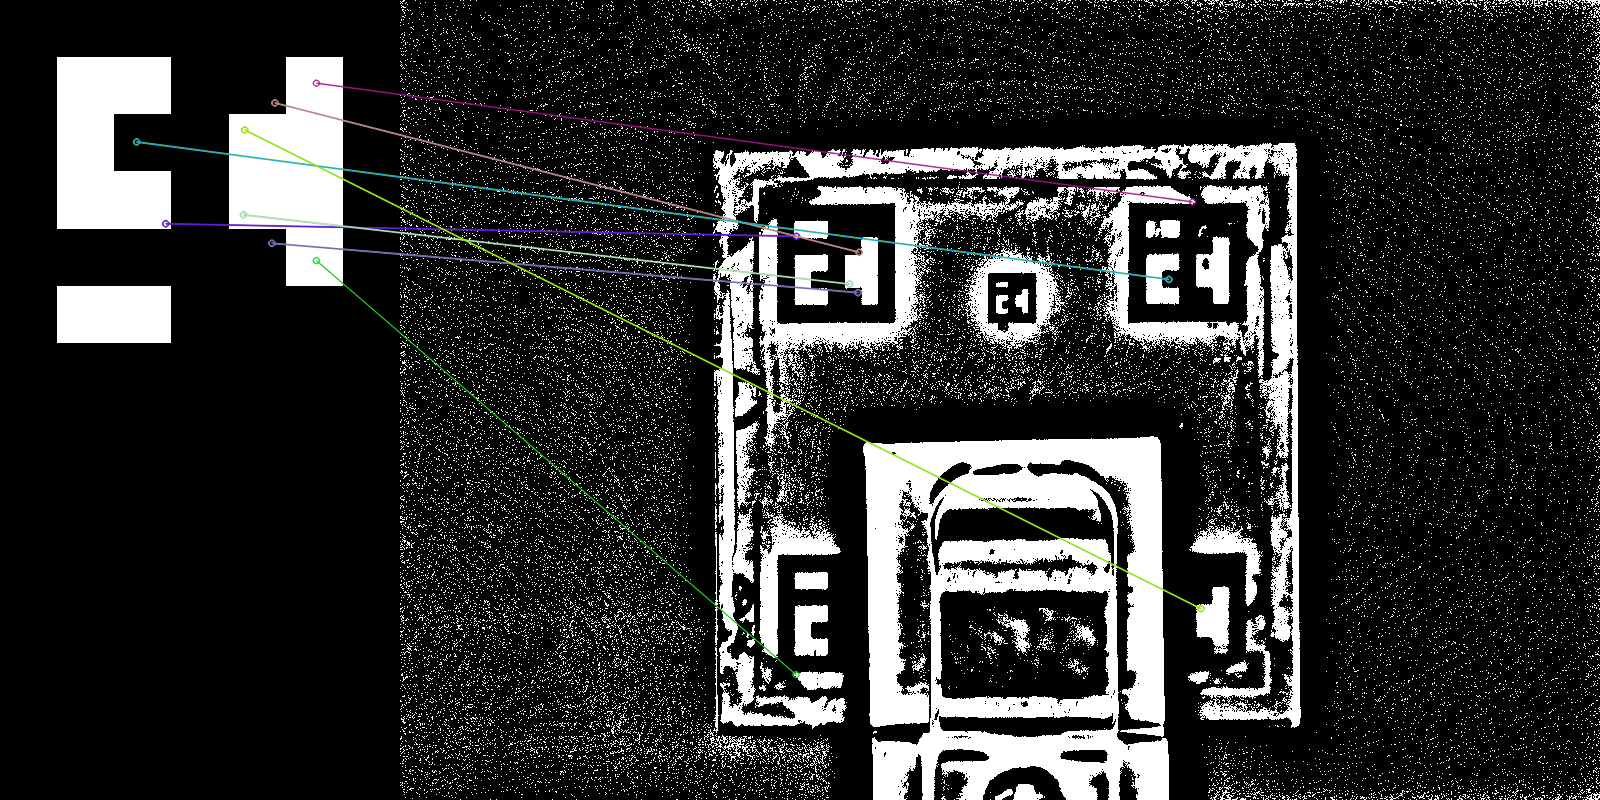
\includegraphics[width=0.65\textwidth]{image/classic_sift_matches}
  \label{fig:classic_sift_matches}
\end{figure}

\begin{figure}
  \caption{Detections of the marker middle using the \ac{SIFT} approach with a sliding window and postprocessing.}
  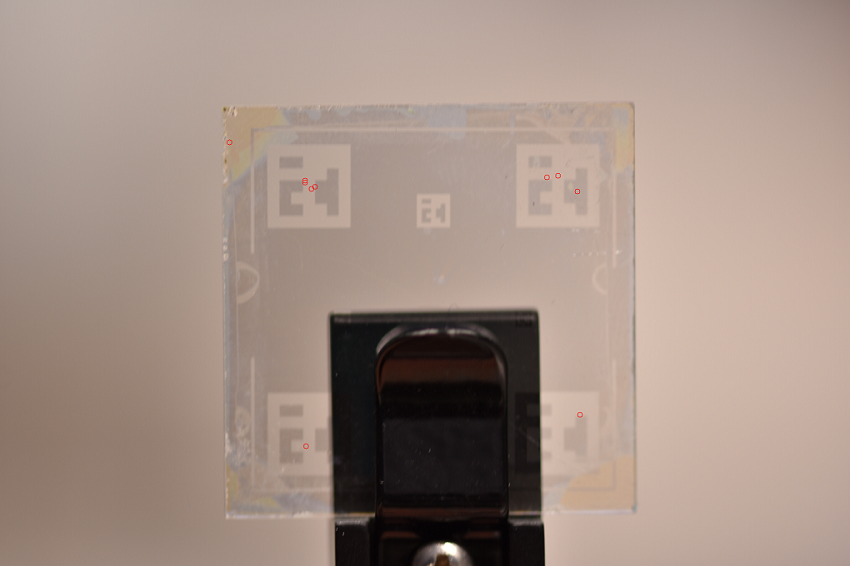
\includegraphics[width=0.5\textwidth]{image/classic_sift_final_matches}
  \label{fig:classic_sift_final_matches}
\end{figure}

\begin{figure}
  \caption{Adaptive thresholding on an image from the test set.}
  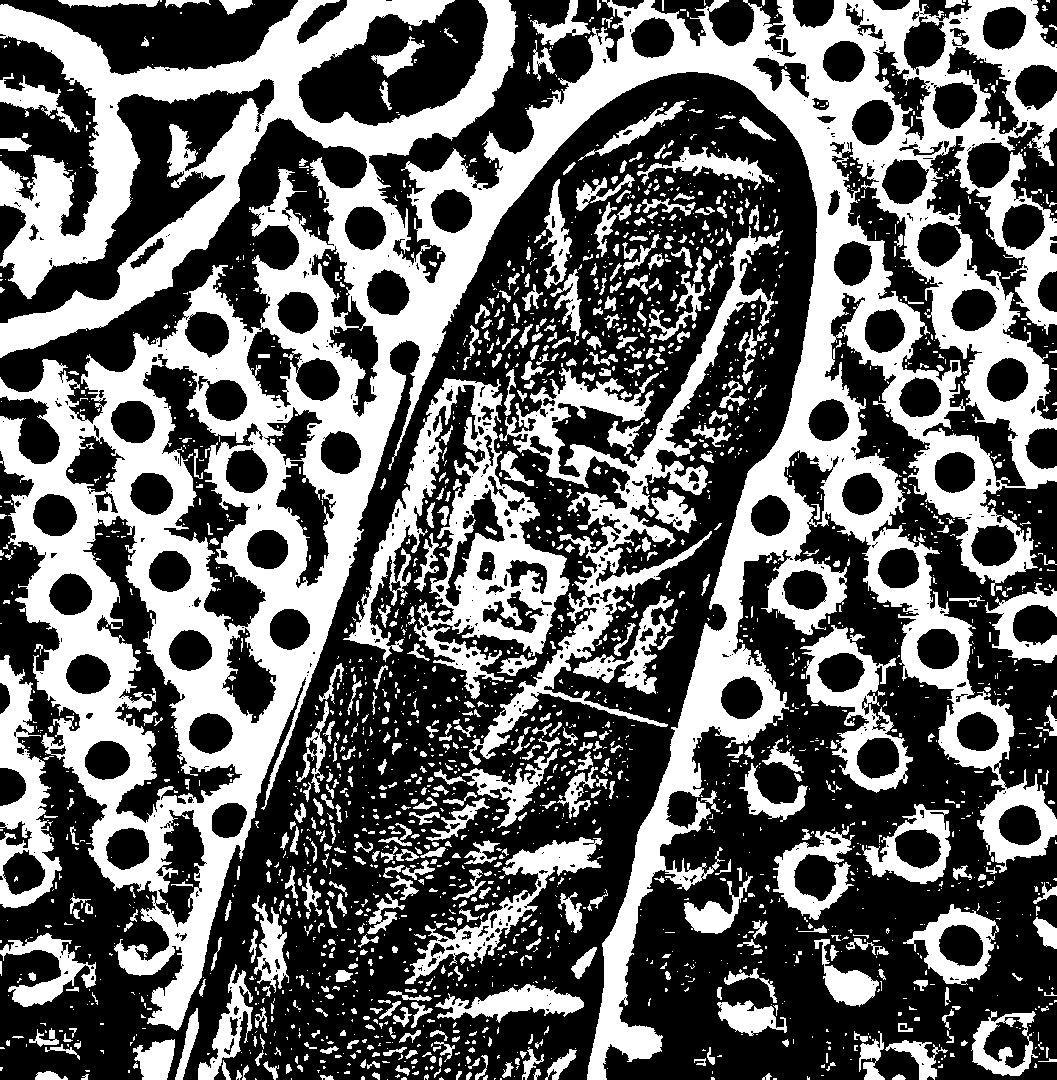
\includegraphics[width=0.4\textwidth]{image/classic_sift_thresh_on_finger}
  \label{fig:classic_sift_thresh_on_finger}
\end{figure}

Since the output of adaptive thresholding on the image in the histogram approach segments the parts of the \ac{ArUco} marker well, as seen in \figureref{fig:classic_sift_matches}, I also used a feature matcher on the thresholded image and a image of the \ac{ArUco} marker to detect the marker positions. Due to familiarity, I used \acp{OpenCV} implementation of \ac{SIFT} with the brute-force matcher for this task. Since feature matching in this way will separate the matches across the repeating marker structures, as seen in \figureref{fig:classic_sift_matches}, I applied a sliding window around the matching process. Finally, the positions of the matches in the image are moved by the difference of their position in the marker image and the middle of the marker image to cluster them. % TODO: Make this more understandable
The results of that process can be seen in \figureref{fig:classic_sift_final_matches}, where the majority of the matches land on or near the middle of a \ac{ArUco} marker in the image. However, when using this matching process on an image of the real test set, nothing is detected, since the thresholded image there does not preserve the structure of the \ac{ArUco} marker enough for the \ac{SIFT} matching, as seen in \figureref{fig:classic_sift_thresh_on_finger}.

\subsection{Conclusion}

While I cannot try out all combinations of data transformations and image algorithms to find the best \ac{ArUco} marker detection algorithm, these attempts do illustrate that finding a machine learning free detection algorithm for this task is a hard problem, which therefore constitutes the usage of neural networks for this usecase.

\section{Software Architecture}

Python has support for the structuring of script files into modules in which data can be primarily exchanged between components through function call arguments. However, for this work I chose to structure the project as loose script files that exchange data primarily through the filesystem. The advantage in that approach is that all intermediate results of the script pipeline necessarily stay in the filesystem and can be used for validation later. Furthermore, should there be an error in the execution of a script later in the pipeline, that script can easily be started again with adapted code and tested on the input data it failed on without having to run all previous steps, such as retraining a model.

\subsection{Data Pipeline Overview}

\begin{figure}
  \caption{Overview of the most important data structures and scripts of the data pipeline from raw data to a dataset. The orange nodes stand for data and blue nodes stand for python scripts.}
  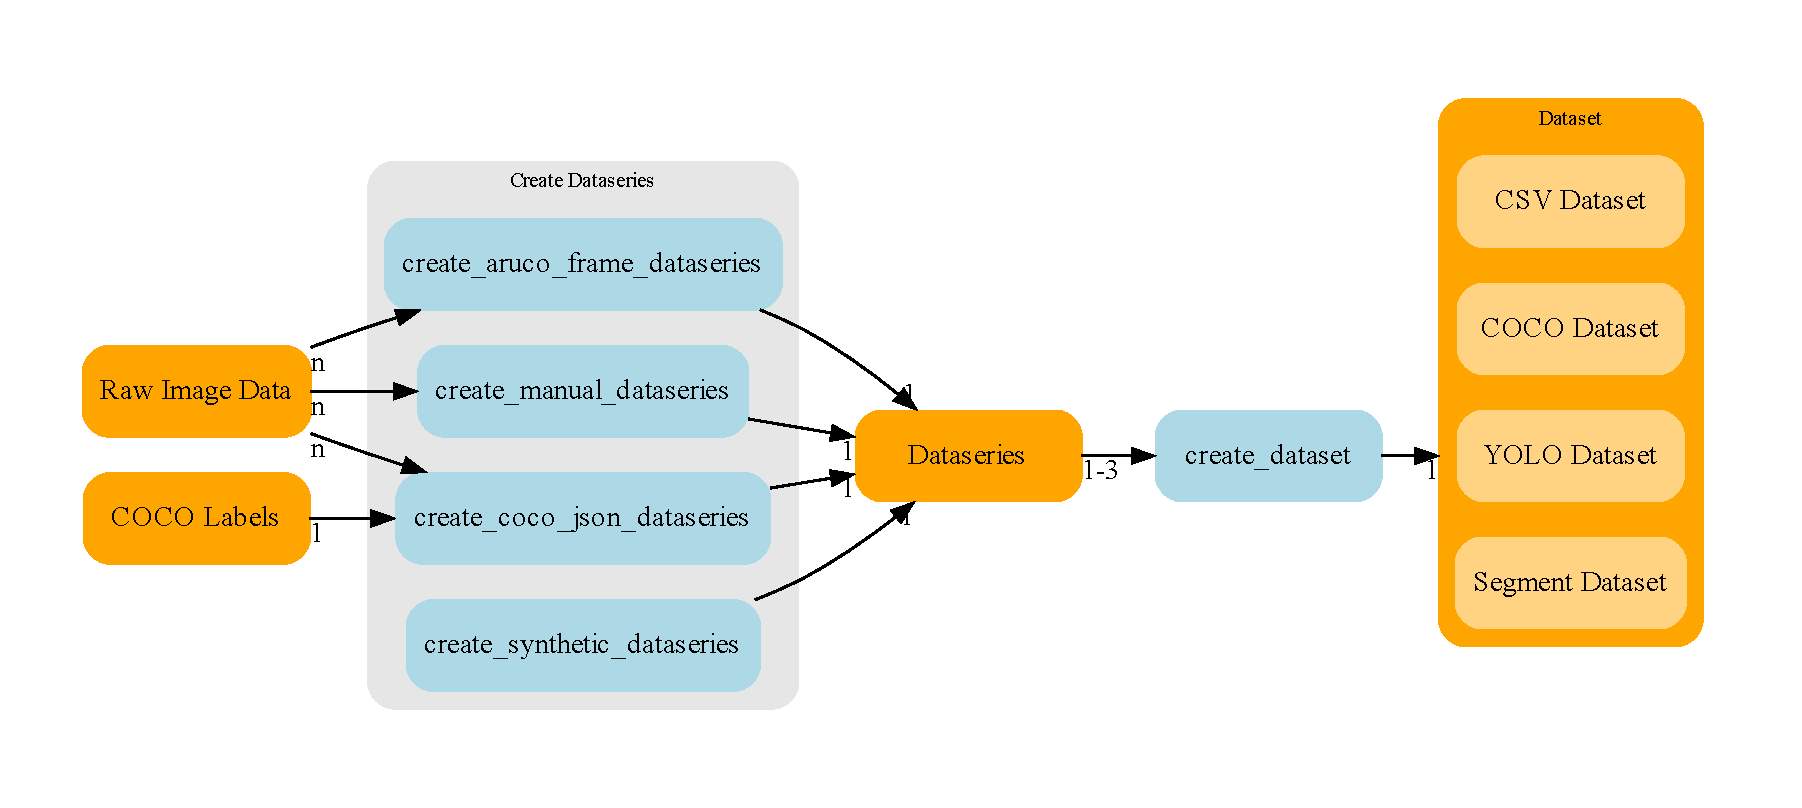
\includegraphics[width=\textwidth]{graph/arch_data}
  \label{fig:arch_data}
\end{figure}

The first part of the script pipeline is visualized in \figureref{fig:arch_data}. It serves four major goals. 

Firstly, it should define a standardized label data type that all dataset types can be build from. This is addressed by the usage of polygons further described in \autoref{sec:label_data_type}.

Secondly, it should allow for a simple way to annotate large amounts of data to keep the labeling workload low. This is addressed by the \texttt{create\_aruco\_frame\_dataseries} script, which is described in more detail in \autoref{sec:auto_annots}.

Thirdly, it should output a range of dataset types such that the data can be easily trained on many predefined \ac{NN} packages and projects to get the best results. This is addressed by the \texttt{create\_dataset} script which builds the data in a variety of dataset structures.

Fourth, it should build augmentations into the data, such that custom augmentations can be tested on different models without having to adapt the dataloader that comes with the model. Most predefined dataloaders and model backbones/heads share few data format standards, which makes changes there time consuming. This is also addressed by the \texttt{create\_dataset} script and described in more detail in \autoref{sec:augs}.

% The overview seen in \figureref{fig:arch_data} shows the various dataset types that are built , addressing the third goal. The  addresses the second goal. Furthermore, augmentations are added in the \texttt{create\_dataset} script, addressing the fourth goal.

The \texttt{create\_synthetic\_dataseries} script seen in \figureref{fig:arch_data} is further described in \autoref{sec:synth_data}.

\subsection{Label Data Type}
\label{sec:label_data_type}

\begin{figure}
  \centering
  \subcaptionbox{Unrotated image and polygon (orange) / bounding box (blue) labels}
     {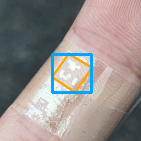
\includegraphics[width=0.3\textwidth]{image/polygon_pog_1}}
  \subcaptionbox{Image and polygon (orange) / bounding box (blue) labels after 50° rotation, as well as the old bounding box data in gray}
     {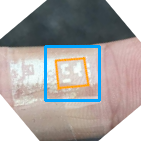
\includegraphics[width=0.3\textwidth]{image/polygon_pog_2}}
  \caption{Two images from the test set showing a polygon label in orange and a bounding box label in blue. After a rotation augmentation operation was applied in image two, the new bounding box label could only be created based on the old labels information. This old label was already too large since it could not capture the rotation of the object. The polygon label, however, can be augmented with the image without losing label accuracy by transforming the polygon points.}
  \label{fig:polygon-good}
\end{figure}

Image augmentation libraries have support for many data types to accommodate for many use cases. However, Albumentations only supports segmentation masks, bounding boxes and keypoints. While segmentation masks are a versatile data structure, both bounding boxes and keypoints can be reduced to polygons. Furthermore, polygons are able to more accurately fit to an objects structure during augmentations as seen in \figureref{fig:polygon-good}. Therefore, I use polygons as labels in dataseries and throughout the augmentations in the \texttt{create\_dataset} script. Afterwards, the bounds of the polygon's vertices can be used to transform it into a bounding box for object detection dataset types or the polygon can be rasterized to create a segmentation mask.

\subsection{Train Pipeline Overview}

\begin{figure}
  \caption{Overview of the most important data structures and scripts of the training pipeline from datasets to \ac{mAP} scores. Here, orange nodes stand for data and blue nodes stand for python scripts.}
  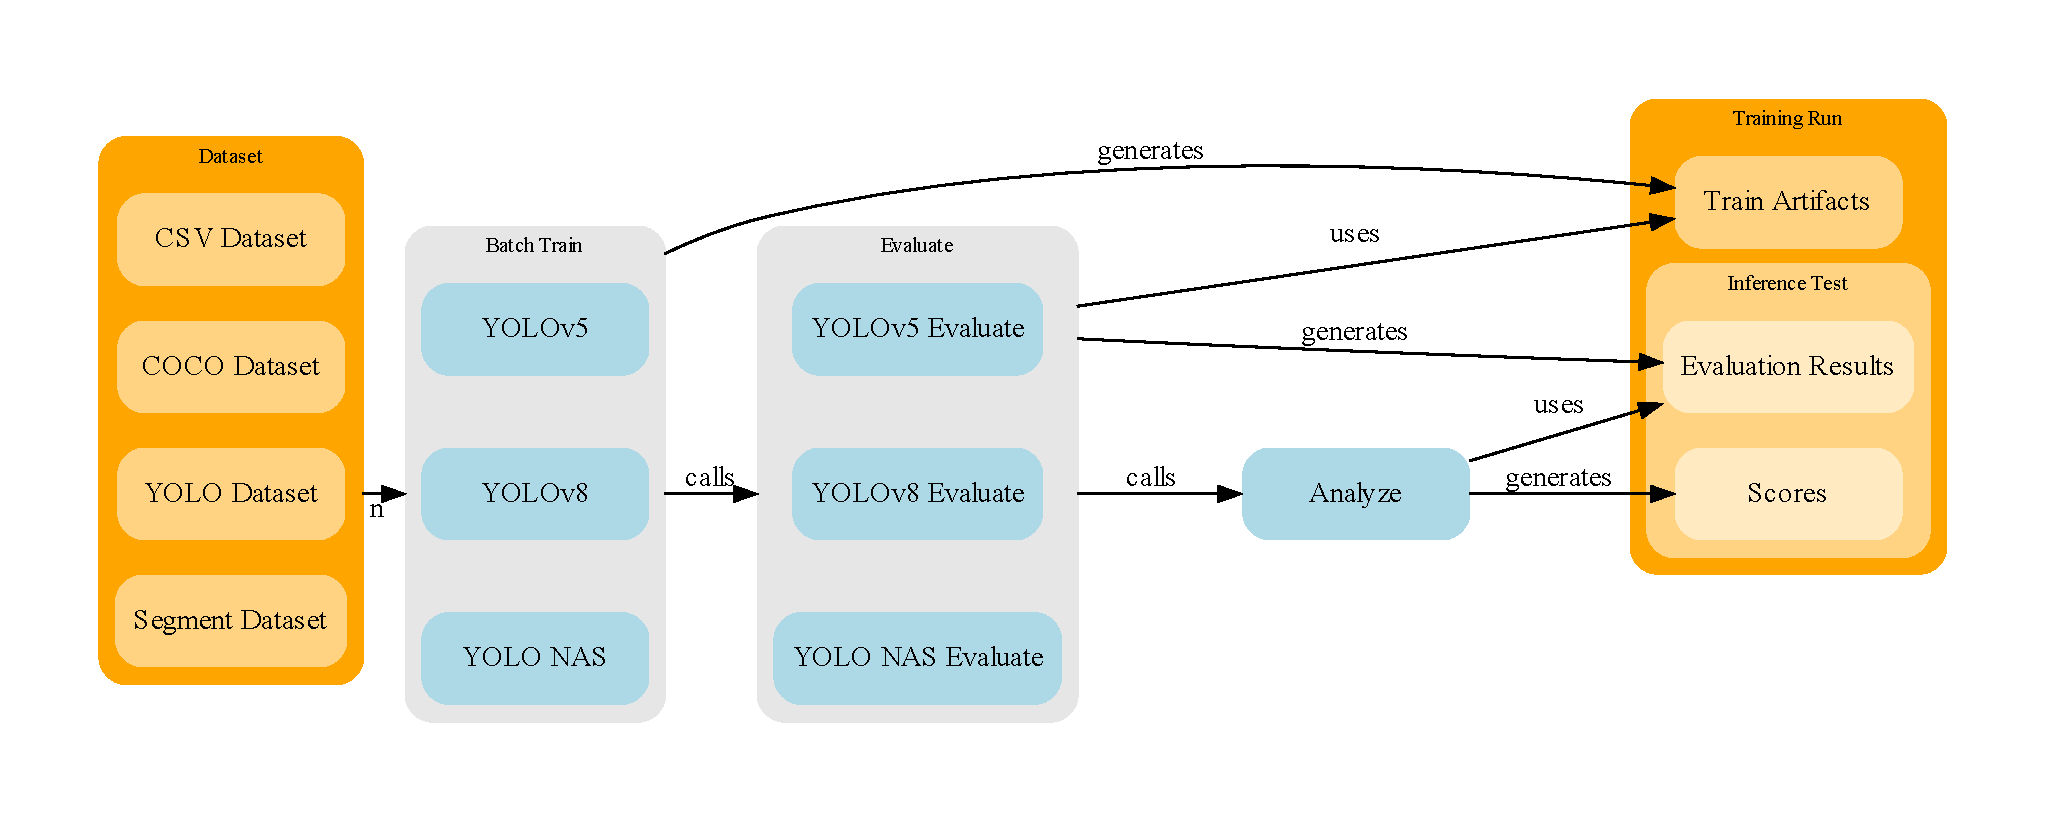
\includegraphics[width=\textwidth]{graph/arch_train}
  \label{fig:arch_train}
\end{figure}

As seen in \figureref{fig:arch_train}, the training pipeline mainly consists of batch train, evaluate and analyze scripts. The batch train and evaluate scripts are implemented for each network source independently due to varying script usage and data formats. The batch train and evaluate scripts are split such that a model can be evaluated using a different set of inference parameters without retraining it. The analyze script implements the \ac{mAP} calculation and is split from the evaluate scripts since it can be implemented independently of each model source. The batch train scripts can handle multiple datasets at once for an ensemble training run.

A training run folder contains the train artifacts, which refers to all files, including the model weights, which are created during training. The relation between training runs and inference tests was omitted in the figure. However, training runs can contain multiple inference tests. Each inference test contains evaluation files which refers to a list of tuples of the networks predicted output and the target output in the xyxy bounding box format in addition to the confidence values, which can be used for the \ac{mAP} calculation, as well as extra files for validation. The scores consist of the calculated VOC 2007, VOC 2010 and \ac{COCO} \ac{mAP} scores, as well as intermediate results of the calculation for validation.

\section{Automated Annotations}
\label{sec:auto_annots}

\begin{figure}
  \centering
  \subcaptionbox{First marked image of a aruco frame dataseries}
     {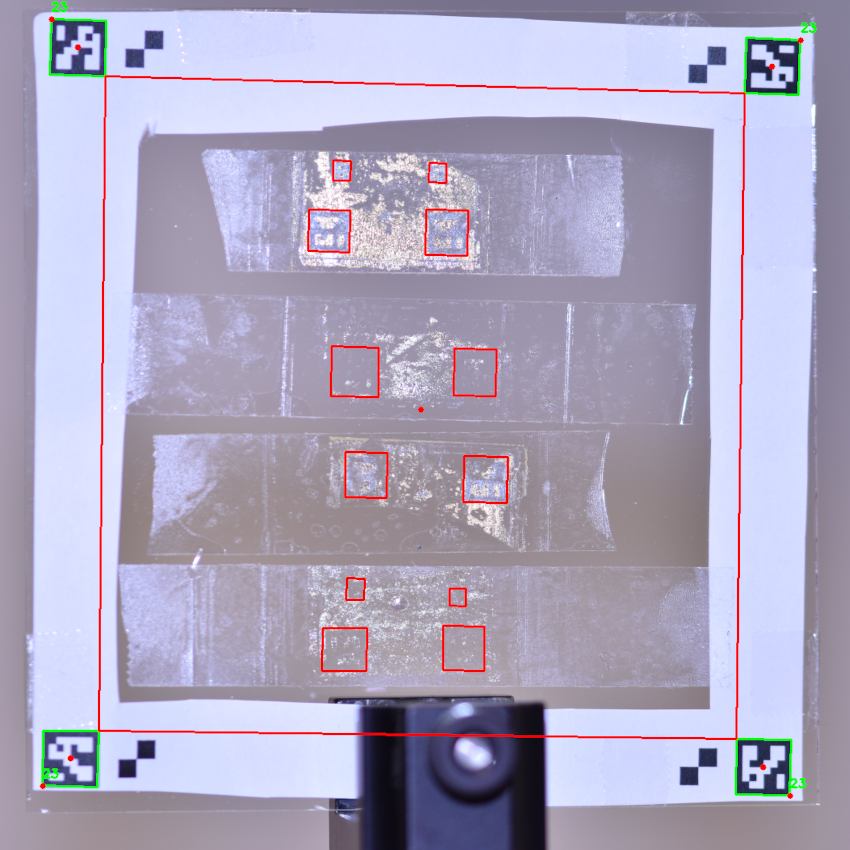
\includegraphics[width=0.45\textwidth]{image/af_markings_1}}
  \subcaptionbox{Later marked image of a aruco frame dataseries}
     {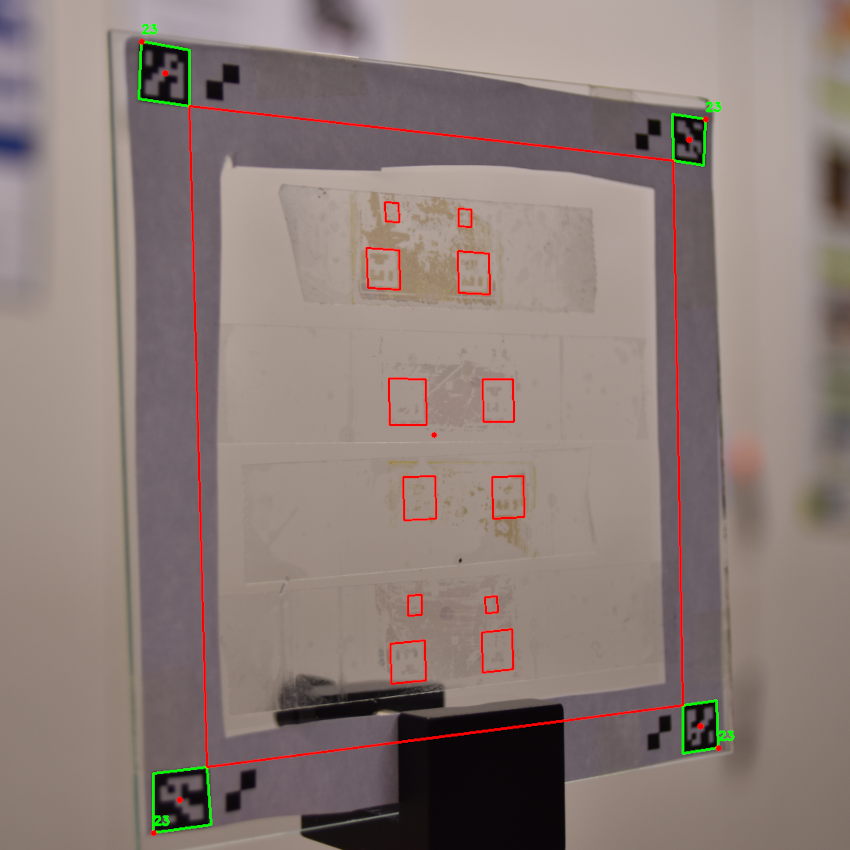
\includegraphics[width=0.45\textwidth]{image/af_markings_2}}
  \caption{Two example images from the validation data of the \texttt{create\_aruco\_frame\_dataseries} script.}
  \label{fig:af_markings}
\end{figure}

To make the annotation of training data faster, we printed 4 \ac{ArUco} markers on the corners of a quadratic paper, cut out the middle and used it as a frame for the actual training data as seen in \figureref{fig:af_markings}. Since the tape containing the markers is on a planar surface, the position of the plane in 3D space can be computed based on the \ac{OpenCV} detectable \ac{ArUco} markers on the paper corners. By manually labeling the first image in such a series of images, where the placement of the markers does not change, the positions of all the markers in the rest of the series can be inferred.

\begin{figure}
  \caption{Position of the \texttt{create\_aruco\_frame\_dataseries} script in the pipeline.}
  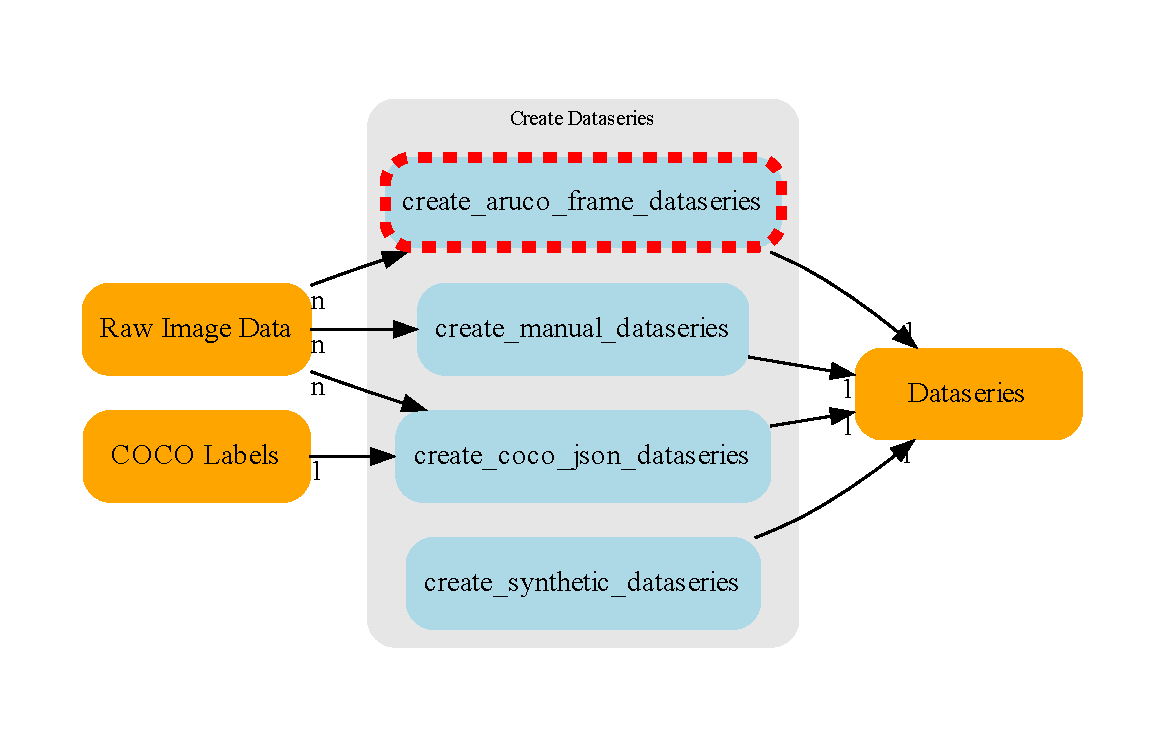
\includegraphics[width=0.65\textwidth]{graph/arch_data_af_focus}
  \label{fig:arch_data_af_focus}
\end{figure}

The position of this script within the pipeline can be seen in \figureref{fig:arch_data_af_focus}. After the script starts, the first image of the image series given in the command line arguments is analyzed by the built-in \ac{OpenCV} \ac{ArUco} detector. Should there be 4 detected markers, the script will attempt to find the inner rectangle which is the largest marked in red in \figureref{fig:af_markings}. For the Homography calculation in the next step, it is important that the corners of the inner rectangle have a stable ordering.

There are two algorithms for finding the inner rectangle. The first one, also called \texttt{legacy\_rect\_finding} in the script, sorts each markers corners that are the closest to the middle into a list based on the quadrant the marker is in the image. Therefore, \texttt{legacy\_rect\_finding} works independent of the orientations of the markers on the paper frame. However, it is dependant on the placement of the markers in the image. 

The second algorithm assumes that all printed \ac{ArUco} markers on the paper frame have the same orientation and that the corner list of the marker is sorted in an u-shape. The latter constraint is already satisfied by the output of the \ac{OpenCV} \ac{ArUco} detector. Every markers corner closest to the image middle is then sorted into the inner rectangle corner list based on the corners index within the markers corner list. %as seen in \autoref{lst:irf}. 
The inner rectangles corners are now sorted in an u-shape as well. The relationship between the indices is visualized in \figureref{fig:inner_rect_indices}. As long as the respective assumptions of the two algorithms hold, they both result in a stable u-shaped ordering of the corners.

\begin{figure}
  \caption{Matching corner indices of the \ac{ArUco} rectangles and the red inner rectangle corners written on the image.}
  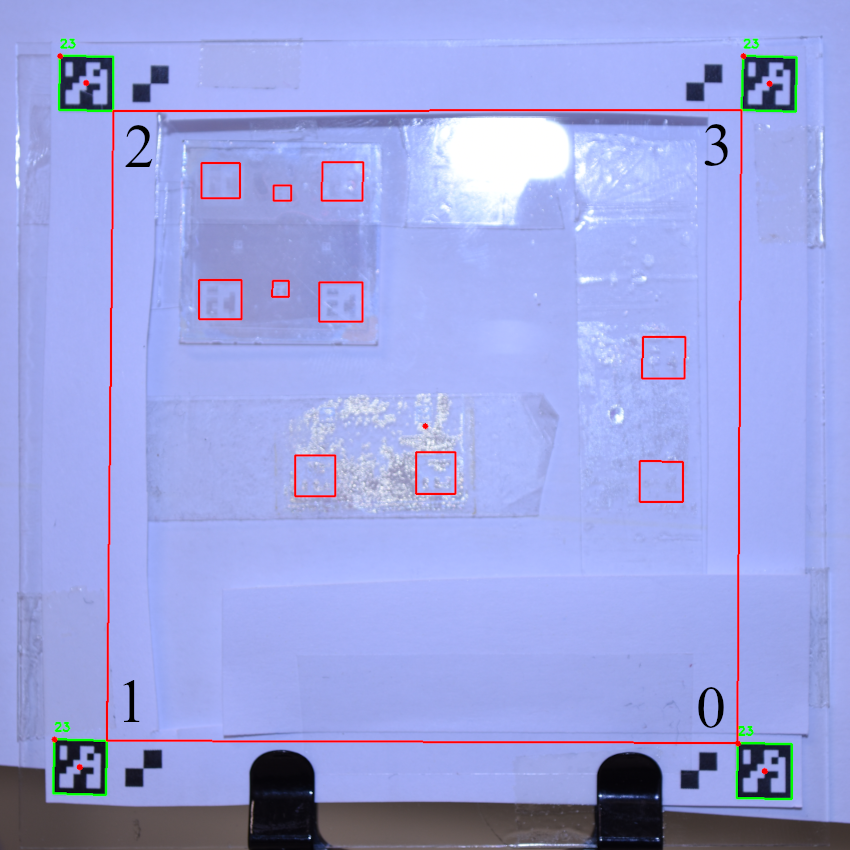
\includegraphics[width=0.5\textwidth]{image/af_markings_3}
  \label{fig:inner_rect_indices}
\end{figure}

% \begin{code}
% \captionof{listing}{Inner Rectangle Finding}
% \label{lst:irf}
% \begin{minted}{python}
%   def find_inner_rect(each_arucos_corners, center):
%     inner_rect = [None, None, None, None]

%     for corners in each_arucos_corners:
%         # Get index of closest corner to image center in ArUco marker rectangle
%         min_i, _ = min([(i, distance(v, center)) for i, v in enumerate(corners)], 
%                        key=lambda x: x[1])
                
%         # The markers corner closest to the middle is the min_i'th vertex of the inner rect
%         inner_rect[min_i] = corners[min_i]
        
%     return inner_rect
% \end{minted}
% \end{code}

Afterwards, a homography from the inner rectangle corners to the points $(0,h), (0,0), (w,0), (w,h)$ is computed, the initial image is transformed using it and the user can label all visible markers on the transformed image in an \ac{OpenCV} \ac{GUI} window.

Once the user is done, the labels are transferred to each other image in the dataseries by finding the \ac{ArUco} frame like before, finding its inner rectangle, computing the homography for it and transforming the user defined labels as polygons onto the image using the user defined points and the two homographies. However, this time the homography is computed the other way around from the points $(0,h), (0,0), (w,0), (w,h)$ to the inner rectangle corners.

\section{Augmentations}
\label{sec:augs}

This section describes the augmentations that were implemented into the \texttt{create\_dataset} script. They were implemented such that the chance of application and their maximum strength can be set through command line arguments. Furthermore, the images are copied such that the original not augmented training images and labels are kept in the dataset at least once and such that only copies are augmented. The number of which can also be changed through command line arguments but is 3 by default. The position of the augmentations in the pipeline is shown in \figureref{fig:arch_data_aug_focus}.

\begin{figure}
  \caption{Position of augmentations in the pipeline.}
  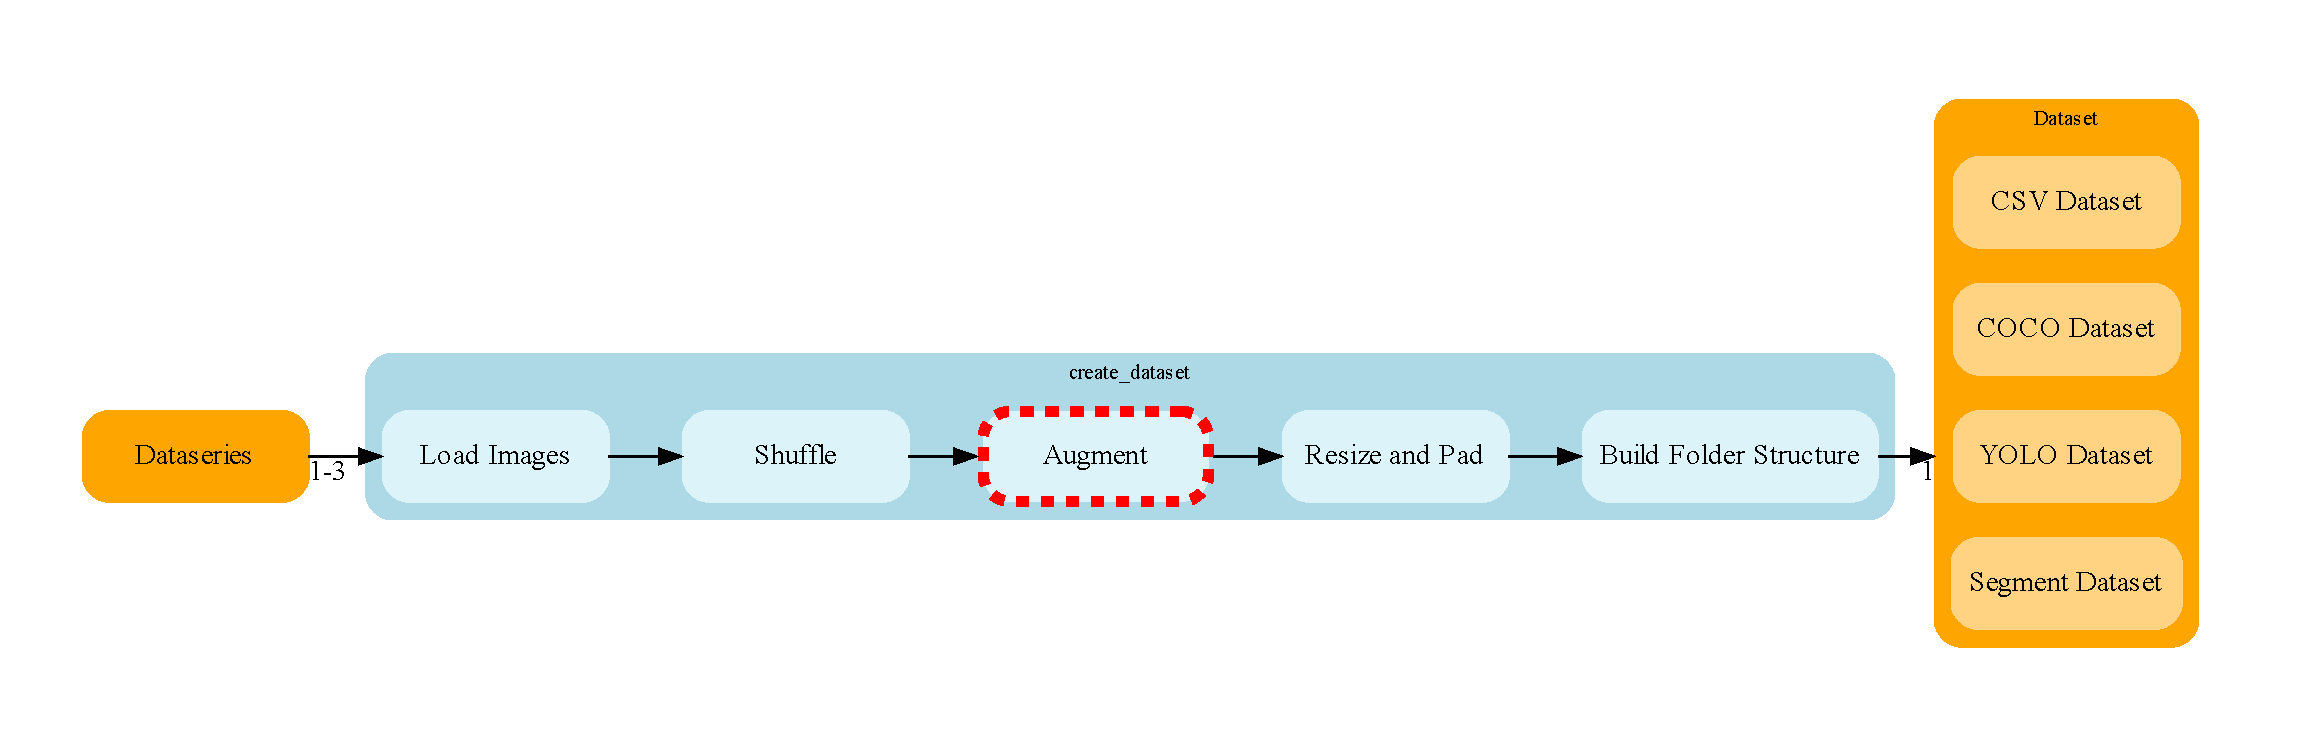
\includegraphics[width=\textwidth]{graph/arch_data_aug_focus}
  \label{fig:arch_data_aug_focus}
\end{figure}

\subsection{Smart Grid Shuffle}

The training data contains series of images with multiple tapes in the same relative positions on the glass plate. However, these relative positions should not be learned, since the trained model should recognize single markers independently of their surroundings. 

One image augmentation that breaks up the overall image structure is grid shuffling and Albumentations already has an implementation for grid shuffling. However, that implementation does not work on bounding boxes, since the grid lines, on which the image is split apart, may also split apart bounding boxes and the objects they describe. This makes sense for Albumentations, which is build to work within dataloaders as a fast augmentation pipeline. However, in this case the performance of the augmentation does not matter as much, since it is build into the dataset before the training. To make grid shuffling work for this case, I adapted it to not split the image on a fixed grid but on gaps between polygon labels. To keep the algorithm simple, all cuts are axis aligned.

\subsubsection{Implementation}

The first part of smart grid shuffle traverses the polygon labels in order of their centroid position on a given axis. Should the distance between the bounding boxes of two polygons on the given axis be larger than a threshold, the image is cut along the other axis and a segment is created, as seen in \autoref{lst:sgs_cut}.

% \begin{algorithm}
%   \SetAlgoLined
%   \KwIn{$I$: the image, $P$ the list of polygon label for the image, $D$ the axis to work in, $p$ the minimum distance between polygons for a cut}
%   \KwOut{$S$: list of segments}
%   $S \leftarrow []$ 

%   sort $P$ ascendingly based on polygon centroid position on axis $D$\;
%   \For{$i\gets0$ \KwTo len($P$)-2}{
%     $d \leftarrow$ distance between $P[i]$ and $P[i+1]$;

%     \uIf{$d$ > $p$}{
%       $e_{Last} \leftarrow S[-1]$.end;

%       $e \leftarrow$ $D$ component of midpoint in area between $P[i]$ and $P[i+1]$;


%     }
%   }
%   \caption{Segment generation part of smart grid shuffling}
% \end{algorithm}

% [caption={Smart Grid Shuffling Algorithm in Pseudocode},captionpos=b,label=lst:sgs_cut]

\begin{code}
\captionof{listing}{Cutting part of smart grid shuffle.}
\label{lst:sgs_cut}
\begin{minted}{python}
# Generate image segments by cutting the image on axis aligned lines between polygon labels
def segment_img(img: Mat, polys: List[Polygon], axis: Literal[0,1], min_cut_distance = 5):
  segments = []
  
  # Sort the polygon labels on the opposite axis the image should be cut in, 0 for x and 1 for y
  polys = sort_polys_in_axis(1 - axis, polys)
  
  # Traverse the polygon labels in order and generate image segments
  for i in range(len(polys)-1):
  axis_distance = distance_between_this_and_next_poly_on_axis(polys, i, axis)

    if axis_distance > min_cut_distance:

      # Get the last and current segment end values on traversed axis 
      last_end = segments[-1].end if len(segments) > 0 else 0
      end = mid_between_poly_bounds(polys, i, axis)

      # Generate segment
      segment_polys = get_polys_in_segment(polys, last_end, end)
      segment_img = img[:, last_end:end] if axis == 0 else img[last_end:end, :]
      segments.append(Segment(end, segment_polys, segment_img))

  # Generate last image segment analogously with end being the image size
  segments.append(last_segment)
  
  return segments
\end{minted}
\end{code}

The second part of smart grid shuffle defines the recombination of the image segments along an axis into a combined image and a combined label list as seen in \autoref{lst:sgs_comb}.

\begin{code}
\captionof{listing}{Segment combination part of smart grid shuffle.}
\label{lst:sgs_comb}
\begin{minted}{python}
def recombine_segments(segments, target_img_size, axis: Literal[0,1]):
  result_img = get_empty_image_of_size(target_img_size)
  result_polys = []

  # Traverse image and place image segments
  pos = 0
  for seg in segments:
    if axis == 0: # x
      result_img[:,pos:seg.end] = seg.img
    else: # y
      result_img[pos:seg.end,:] = seg.img
        
    result_polys.append(seg.polys)
    pos = seg.end
    
  return aug_image, aug_polys
\end{minted}
\end{code}

The last part uses the defined segment cutting and recombination operations to first segment the image along the y-axis and shuffle the resulting segments. Each segment is then further segmented on the x-axis, shuffled and recombined. Finally all y-axis segments are recombined and returned.

\begin{code}
\captionof{listing}{Segment combination Part of smart grid shuffle.}
\label{lst:sgs_main}
\begin{minted}{python}
# Main method
def smart_grid_shuffle(img, polys: List[Polygon], img_size_wh):
  # First segment in y 
  segments_y = segment_img(img, polys, 1)

  # Shuffle the resulting y-segments
  random.shuffle(segments_y)

  # Segment all segments_y on the x axis
  for segment_y in segments_y:
    segments_x = segment_img(segment_y.img, segment_y.polys, 0)
    
    # Shuffle inner segments
    random.shuffle(segments_x)
    
    # Rebuild the current y-segment from the inner x-segments
    segments_img, segments_polys = recombine_segments(segments_x, segment_y.size(), 0)
    segment_y.img = segments_img
    segment_y.corners = segments_polys

  # Return recombined y-segments
  return recombine_segments(segments_y, img_size, 1)
\end{minted}
\end{code}

\subsubsection{Example}

\begin{figure}
  \centering
  \subcaptionbox{before augmentation}
     {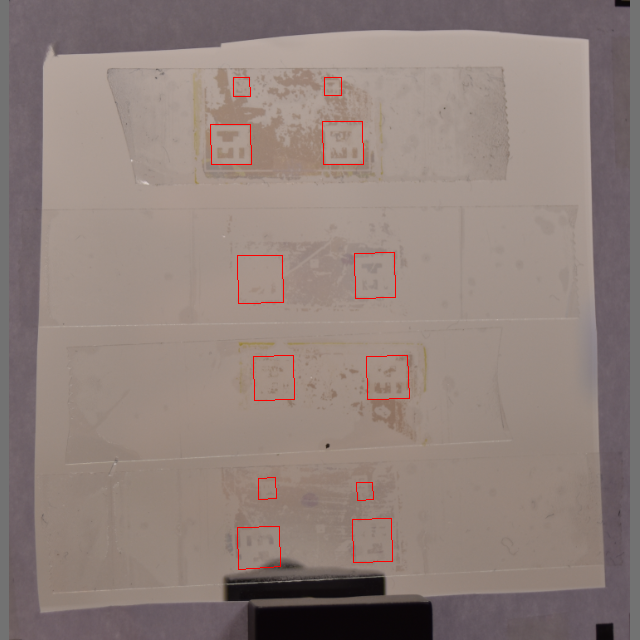
\includegraphics[width=0.45\textwidth]{image/aug_sgs_before}}
  \subcaptionbox{after augmentation}
     {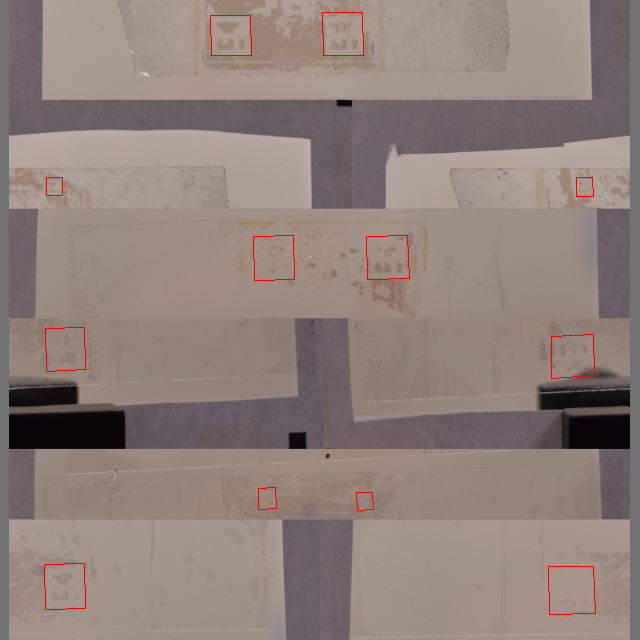
\includegraphics[width=0.45\textwidth]{image/aug_sgs_after}}
  % \subcaptionbox{before augmentation}
  %    {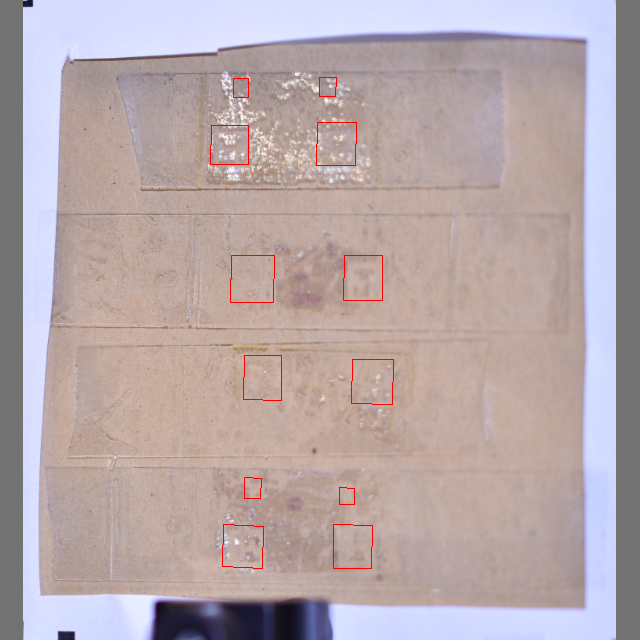
\includegraphics[width=0.45\textwidth]{image/aug_sgs_before2}}
  % \subcaptionbox{after augmentation}
  %    {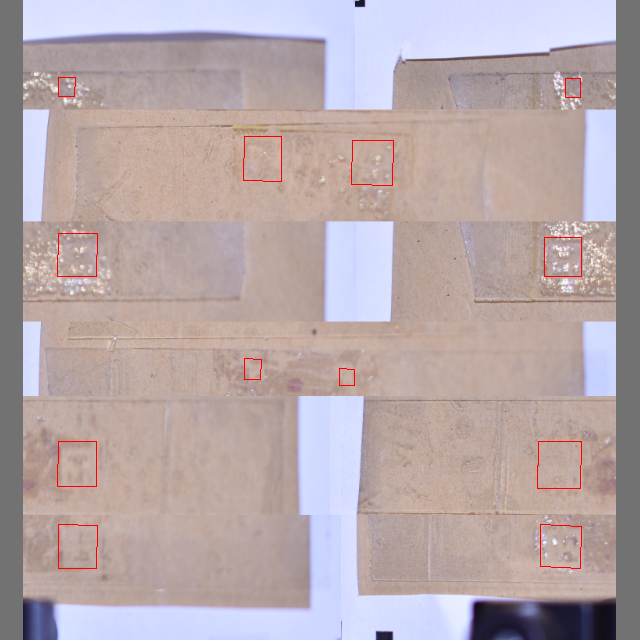
\includegraphics[width=0.45\textwidth]{image/aug_sgs_after2}}
  \caption{An example for smart grid shuffle on a training image.}
  \label{fig:aug_sgs_example}
\end{figure}

The smart grid shuffle augmentation cuts and reassembles the image such that as much of the possibly important surrounding pixels of the polygon labels are preserved, but that still removes any reoccurring patterns in the image, in which the labels may be arranged by, as seen in \figureref{fig:aug_sgs_example}.

\subsection{Label Dropout}
\label{sec:aug_ld}

\begin{figure}
  \centering
  \subcaptionbox{before augmentation}
     {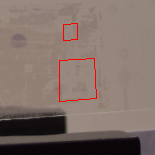
\includegraphics[width=0.3\textwidth]{image/aug_pld_before}}
  \subcaptionbox{after augmentation}
     {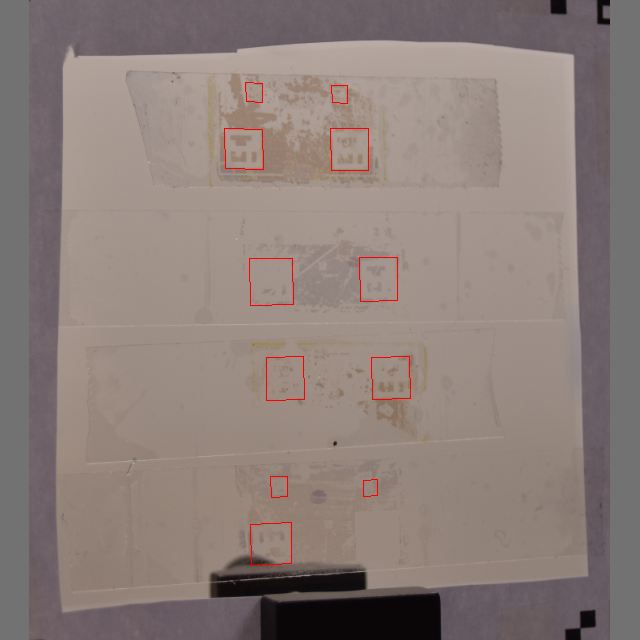
\includegraphics[width=0.3\textwidth]{image/aug_pld_after}}
  \caption{An example for label dropout on a cropped part of a training image.}
  \label{fig:aug_pld_example}
\end{figure}

To further prevent the model from fitting to certain label arrangements in the image, the label dropout augmentation randomly chooses a label, removes the associated marker from the image and removes the label entry. The marker is removed from the image by taking its polygon, scaling it around its centroid by a factor of 1.2 and rasterizing the result on the image using the color on the image at the polygons centroid position. The result of that operation can be seen in \figureref{fig:aug_pld_example}.

\subsection{Homogeneous Matrix Transform}

Rotation and perspective transformations are both combined into a homogeneous matrix transform step to prevent code duplication and to improve performance since this step requires postprocessing.

For most augmentations there is a chance setting and possibly a strength setting depending on the augmentation. Here, the available settings are the chance for a rotation of 90 degree multiples, the chance for rotation of any angle, the maximum rotation angle, the chance for perspective transform and the maximum perspective transformation strength. Firstly, all settings are build into two transformation matrices and both are combined. Then the resulting matrix is used to transform the image as well as the polygon label vertices, as seen in \figureref{fig:aug_mat_example}.

\begin{figure}
  \centering
  \subcaptionbox{before augmentation}
     {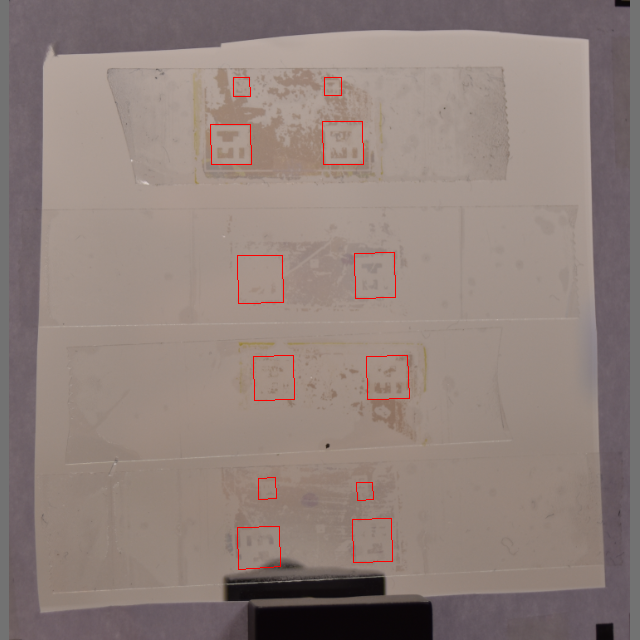
\includegraphics[width=0.45\textwidth]{image/aug_mat_before}}
  \subcaptionbox{after augmentation}
     {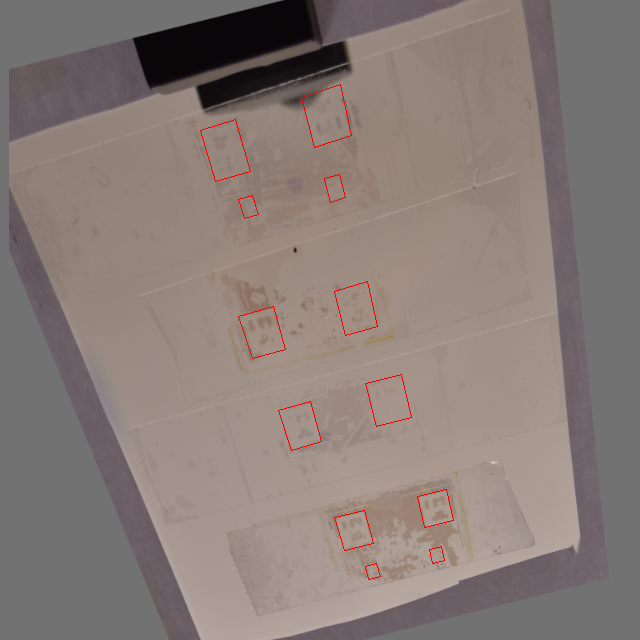
\includegraphics[width=0.45\textwidth]{image/aug_mat_after}}
  \caption{An example for matrix transform augmentation on a training image.}
  \label{fig:aug_mat_example}
\end{figure}

\subsubsection{Out of Bounds Cases}
\label{sec:oob}

After the transformation, cases of \ac{OOB} labels have to be handled, as labels may be rotated out of the visible image area. I defined a minimum visibility threshold at 60\%, such that all markers which should be detected are still clearly visible. To compute visibility, the intersection of the label polygon and the image bounds polygon is computed using Shapely. Visibility is then defined as the area of the intersection polygon divided by the area of the original label polygon. This computation is similar to the \ac{IoU} definition or to albumentations visibility calculation on bounding boxes\footnote{\url{https://albumentations.ai/docs/getting_started/bounding_boxes_augmentation/}, accessed on 05.11.2023}. Should the resulting visibility be lower than the threshold, the label entry is discarded from the list of label entries and the remaining area in the image, in which the marker was, is painted over. The overpainting works exactly like label dropout described in \autoref{sec:aug_ld}. Should it pass the visibility check but still intersect with the image border, the label polygon is set to be the intersection from earlier, effectively clipping it within the image space.

\subsection{Random Crop}

\begin{figure}
  \centering
  \subcaptionbox{before augmentation}
     {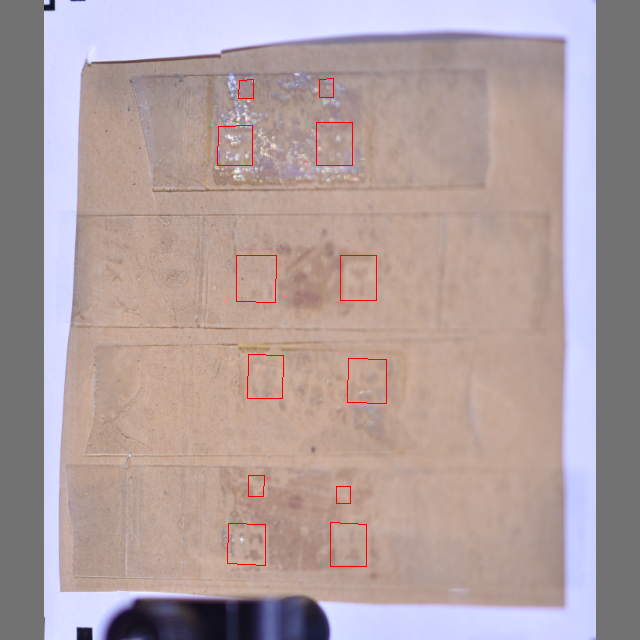
\includegraphics[width=0.45\textwidth]{image/aug_rc_before}}
  \subcaptionbox{after augmentation}
     {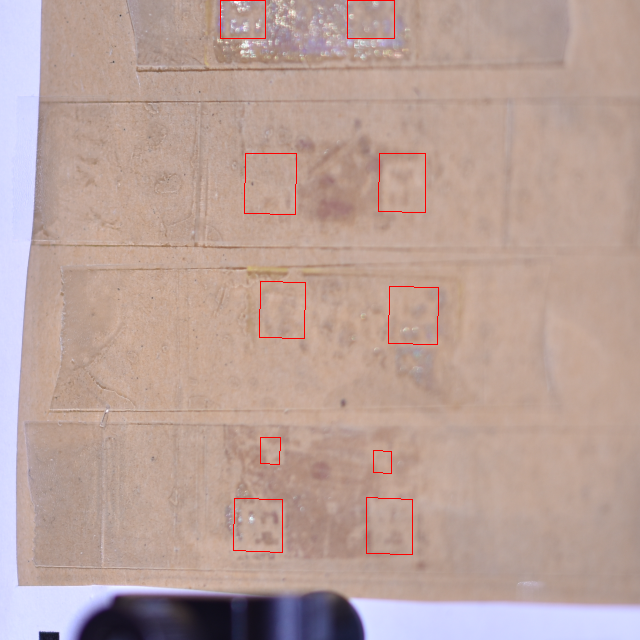
\includegraphics[width=0.45\textwidth]{image/aug_rc_after}}
  \caption{An example for random crop on a training image.}
  \label{fig:aug_rc_example}
\end{figure}

The pipeline implements also a random crop, which crops an area of the datasets target image size out of the input image and moves the labels accordingly as seen in \figureref{fig:aug_rc_example}. Since this augmentation can also leave labels out of bounds, the same postprocessing is applied on the resulting labels as described in \autoref{sec:oob}.

\subsubsection{Augmentation Versions}

\begin{figure}
  \centering
  \subcaptionbox{before augmentation}
     {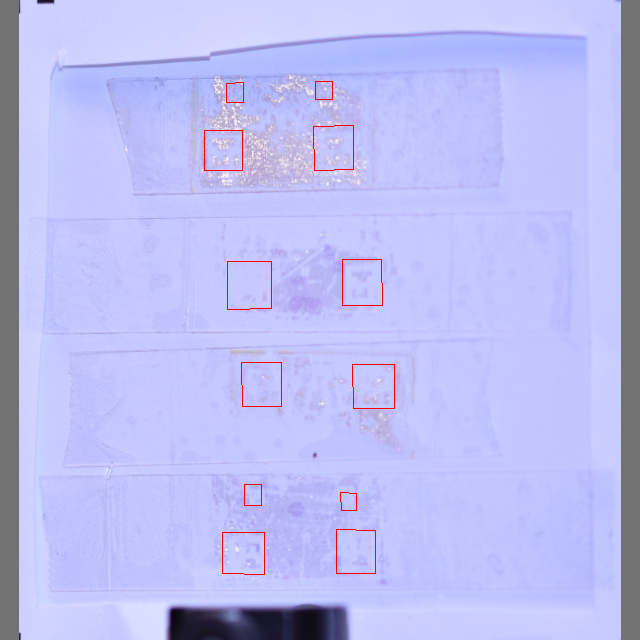
\includegraphics[width=0.45\textwidth]{image/aug_rc2_before}}
  \subcaptionbox{after augmentation}
     {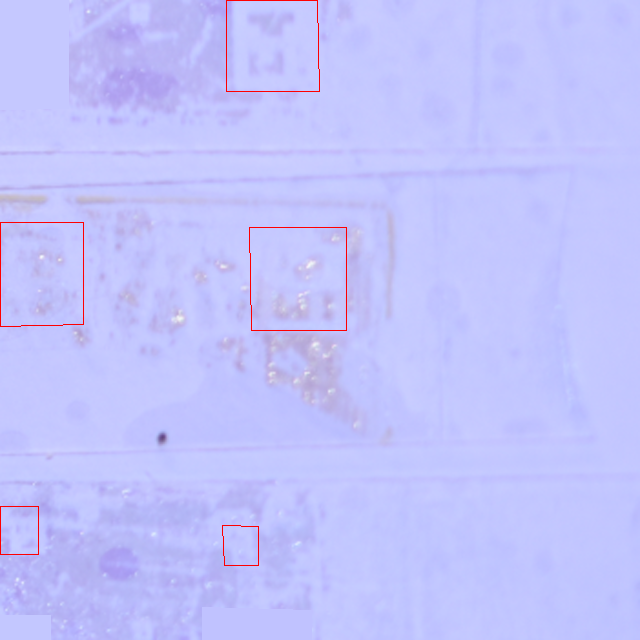
\includegraphics[width=0.45\textwidth]{image/aug_rc2_after}}
  \caption{An example for random crop v2 on a training image. Image (b) also shows how out of bounds labels that do not pass the visibility check are overdrawn. This is done such that the residue of the marker on the image that is without label does not introduce a false negative into the training data, as described in \autoref{sec:oob}.}
  \label{fig:aug_rc2_example}
\end{figure}

The data pipeline also builds \ac{JSON} files into the dataset folder to make the whole dataset build process retraceable. Because of that, I did not change augmentations besides bug fixes once they were implemented, such that the training artifacts including the \ac{JSON} files stay as backwards compatible as possible. 

In this case, I also built a random crop which crops an area of variable size out of the source image and then rescales that cropped part to the target size, which is therefore implemented as its own augmentation: random crop v2. Examples for random crop v2 can be seen in \figureref{fig:aug_rc2_example}. 

Splitting the augmentations in versions this way also has the advantage that the following evaluation can detect how much better a new version of an augmentation performs or if there is regression.

\subsection{Label Move}

\begin{figure}
  \centering
  \subcaptionbox{before augmentation}
     {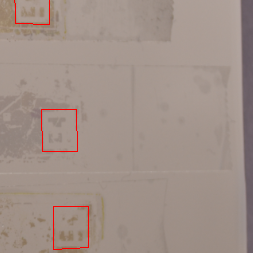
\includegraphics[width=0.3\textwidth]{image/aug_lm_before}}
  \subcaptionbox{after augmentation}
     {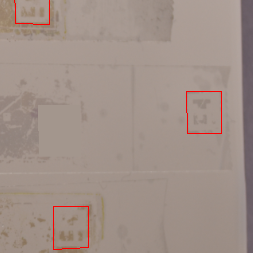
\includegraphics[width=0.3\textwidth]{image/aug_lm_after}}
  \caption{An example for label move on a cropped part of a training image.}
  \label{fig:aug_lm_example}
\end{figure}

Label move works similar to label dropout, as described in \autoref{sec:aug_ld}. However after removing the label from the image, it and its marker image structure is reinserted at a different place in the image, as seen in \figureref{fig:aug_lm_example}. 

Since inserting of images into other images in OpenCV works by copying slices, only \ac{AABB} areas can be inserted at once. However when reinserting the labels image structure at another position, only the \ac{ArUco} marker structure should be inserted and not the surrounding image content. Therefore before inserting the labels image structure back, a mask is applied to it. That mask is the labels polygon rasterized in white onto a black binary image. Using the mask as transparency weights, the labels image structure is then reinserted at the new position.

\subsubsection{Label Move v2}

\begin{figure}
  \centering
  \subcaptionbox{before augmentation}
     {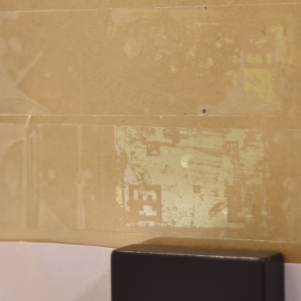
\includegraphics[width=0.3\textwidth]{image/aug_lm2_before}}
  \subcaptionbox{after label move augmentation}
     {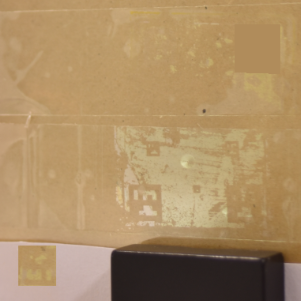
\includegraphics[width=0.3\textwidth]{image/aug_lm2_after_old}}
  \subcaptionbox{after label move v2 augmentation}
     {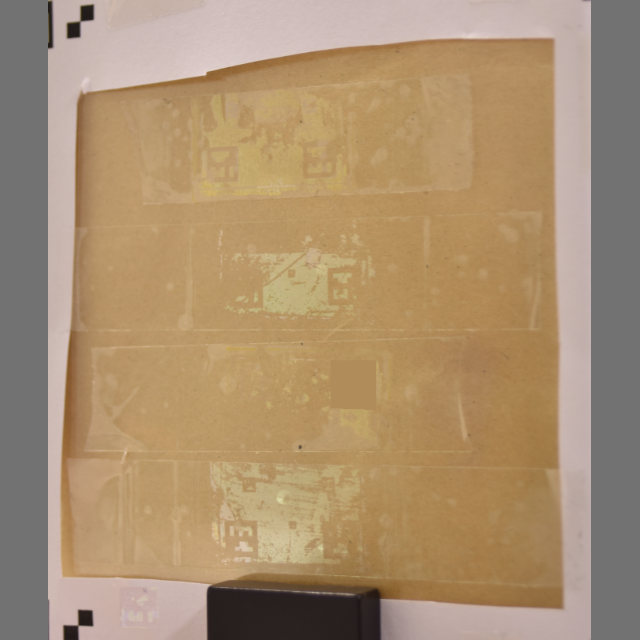
\includegraphics[width=0.3\textwidth]{image/aug_lm2_after}}
  \caption{An example for label move v2 on a cropped part of a training image. Here, the label is moved from the middle of the image to the bottom left. Despite the different background, the color differences is not as noticeable in label move v2. Label borders are not drawn here to make the border differences of the augmentations more visible.}
  \label{fig:aug_lm2_example}
\end{figure}

The second version of label move has two additions to the operations of label move. 

Firstly, the color of the labels image structure is roughly adapted to the target positions color. For this, both the average RGB values of the image target area slice and the average RGB values of the labels image structure are computed. Then, each pixel of the labels image structure is recolored based on the difference of the average RGB values before it is reinserted into the image.

Secondly, gaussian blur is applied to the mask which is a rasterized version of the labels polygon. Due to this change, the inserted labels image structure does not have strong contours anymore and gets a small color transition at its borders.

These changes help the reinserted label blend in in its new position, as seen in \figureref{fig:aug_lm2_example}.

\subsection{Black Dot}

\begin{figure}
  \centering
  \subcaptionbox{before augmentation}
     {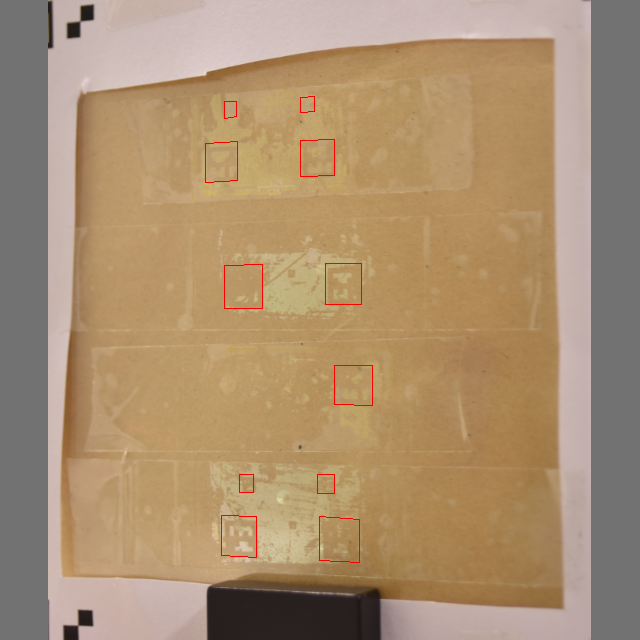
\includegraphics[width=0.45\textwidth]{image/aug_bd_before}}
  \subcaptionbox{after augmentation}
     {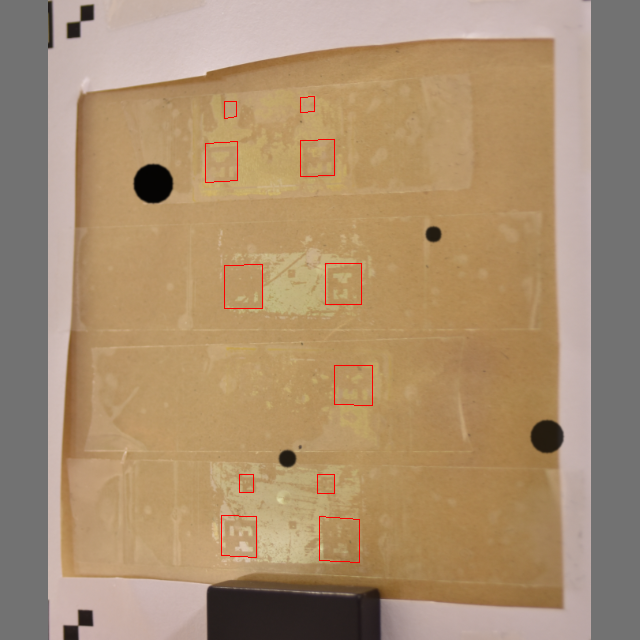
\includegraphics[width=0.45\textwidth]{image/aug_bd_after}}
  \caption{An example for black dot augmentation on a training image.}
  \label{fig:aug_bd_example}
\end{figure}

A reoccurring issue with the application of \ac{SAHI}, which is discussed in more detail later, is that dark objects in the test data were repeatedly and with large confidence misidentified as markers. To make sure that the network learns that dark areas in the image are not markers, I added an augmentation which adds black dots on parts of the image without a marker. 

After the augmentation function is invoked, at least one black dot is added. Afterwards there is a 40\% chance that another black dot is added. If another black dot is added, there is another 40\% chance for one more black dot and so on. While this could continue forever, it gets progressively more unlikely to go on after each iteration. 

The insertion of black dots works similarly to label move, with the difference that a completely black image is inserted and that the mask is a circle. Furthermore, like in label move v2, the mask is blurred using gaussian blur to create a color transition.

An example of black dot aug can be seen in \figureref{fig:aug_bd_example}.

\subsection{Label Curving}
\label{sec:label_curving}

\begin{figure}
  \centering
  \subcaptionbox{before augmentation}
     {\includegraphics[width=0.3\textwidth]{image/aug_lc_before}}
  \subcaptionbox{after augmentation}
     {\includegraphics[width=0.3\textwidth]{image/aug_lc_after}}
  \caption{An example of label curving augmentation on a cropped part of a training image.}
  \label{fig:aug_lc_example}
\end{figure}

Another reoccurrence in the test data is that the tape with the markers was rolled around a finger. Due to the nature of the training data, this case is currently not included in the fitting process. The label curving augmentation should therefore mimic the curved labels.

This augmentation again works similar to label move. However, in this case the label is not moved anywhere. It is cut out and modified using \acp{OpenCV} \texttt{remap} function. \texttt{remap} takes, besides other parameters, two arrays, which represent the x and y coordinates each pixel should be mapped to. In this case, the x coordinates stay the same but the y coordinates are mapped based on a half circle function to mimic the pixel displacement on a curved surface. The middle and the width of the half circle are randomly chosen. Alongside the image cutout, the label vertices are also transformed using the vector field as \texttt{remap}, such that the label is still located over the image structure. The polygon cannot fully capture the curving without new vertices. However, since the polygons are transformed into bounding boxes in most cases this is not a problem. An example of label curving can be seen in \figureref{fig:aug_lc_example}.

\subsection{Gaussian Noise}

While augmentations that work with labels needed to be implemented specifically for this pipeline due to the label datatype, pixel level augmentations already defined in other libraries also work here. The gaussian noise augmentation from Albumentations is therefore used here\footnote{\url{https://albumentations.ai/docs/api\_reference/augmentations/transforms/\#albumentations.augmentations.transforms.GaussNoise}, accessed on 06.11.2023}. 

Gaussian noise adds noise to each pixel in the image, with the strength of the noise being given by the normal distribution. Here, gaussian noise is used to get a different result from the same training configuration even if the training run otherwise works fully deterministic, such that the quality of a training configuration can be more accurately assessed.

% TODO?: \section{Synthetic Data}

\section{Inference}

\begin{figure}
  \caption{Position of evaluation inference in the pipeline.}
  \includegraphics[width=0.75\textwidth]{graph/arch_train_eval_focus}
  \label{fig:arch_train_eval_focus}
\end{figure}

The inference on test data using previously trained models happens in the evaluation scripts, as shown in \figureref{fig:arch_train_eval_focus}. The inference can be optimized using additional filters and other techniques. 

\subsection{SAHI}

One such technique is \ac{SAHI}. 
%However, since each type of model has its own evaluate script, because each type of model works slightly differently, certain techniques have to be implemented separately. Therefore, \ac{SAHI} is currently not supported for \ac{YOLO}-NAS within this project. 
I set the \ac{SAHI} window size to $640 \times 640$ pixels since this is the native input size for the used \ac{YOLO} models. Furthermore, I used a window overlap of 20\% on the x and y axis.

\subsection{Bounding Box Filters}

%Furthermore, the bounding boxes from the inference results can be filtered independently of the model they come from. 
The application of \ac{SAHI} can result in an increased amount of false detections along the border of the image. To prevent this, the size of a border along the the image bounds can be set. All bounding box predictions that fall within this border are filtered out. Additionally to filter predictions which are not square enough, %, which the \ac{ArUco} marker usually are, 
a minimum squareness can be set. Squareness is here defined as $$ 
s(w,h)=
\begin{dcases}
    \frac{w}{h}, & \text{if } w\leq h\\
    \frac{h}{w}, & \text{otherwise}
\end{dcases} $$ where $w$ refers to the bounding boxes width and $h$ to its height. Due to the definition, the squareness score always lies between 0 and 1.

\subsection{Foreground Mask}

Since markers in the images are usually part of the foreground, a pretrained foreground segmentation network could help improve the detection scores.
To test this, I added support for masking of bounding box predictions with predefined masks. Since this is just for testing, this approach is not implemented fully into the pipeline. For the bounding box filtering, the area of the bounding box is cut out of the mask image and the maximum pixel value of the area is checked against a minimum threshold. %Using the average instead of the maximum pixel value lead the lower scores.

% TOxDO?: \section{Plotting}

\section{Automated Ensembles}

Given a set of dataseries as base and parameters for dataset creation, training and inference, the entire process for ensemble learning can now be automated. Furthermore, by starting multiple batch train instances and giving each information about its worker index and the total worker count, the training load for multiple runs on different datasets can be split among multiple processes and \acp{GPU}. Finally, given a consistent naming scheme for the training runs, the score results can also be automatically plotted.

The top level scripts necessary for this are currently only implemented to work with the \ac{MIP} server structure, but could be ported to any \ac{GPU} server with Docker support.

\section{Hyperparameter Optimization}
\label{sec:hyper_opt}

To find an optimal combination of augmentations from the implemented ones, a hyperparameter optimization is implemented using Hyperopt. 

More precisely, the search space for this application of Hyperopt contains the chances for each augment to be applied on an image during dataset generation. Furthermore, the maximum strengths of augments that define one, such as the maximum rotation angle for the rotation augment, are also part of the search space. 

The epochs that should be trained for are also part of the search space. The validation data in the datasets used here can be similar to the training data since both are formed from \ac{ArUco} frame dataseries. The hyperparameter optimization can therefore choose an earlier stopping point for the training, should further training not increase the score on the given test data. 

% Finally, the random seed for the dataset creation is also part of the search space, such that 

The randomness for each configuration of augmentation parameters could be handled by %not including the random seed in the search space and instead 
doing an ensemble run with random random seeds for a given configuration inside the objective function. Doing multiple training runs on an configuration and taking the average score should converge towards the actual average score for that configuration and therefore lead to more stable optimization. However, the hyperparameter optimization is already time consuming and pairing the optimization with ensemble runs would increase the needed runtime further. I therefore chose to model the random seed as part of the search space similarly to how Bethard proposes it for model performance comparisons \cite{bethard2022need}. Due to this, the best training run from the optimization is also fully reproducible given the optimal found search space values. 

\section{Marker Corner Detection}

This section describes the development of the second part of the detection pipeline. After the areas of interest were found by a fitted model which works on the whole image, this part finds the corner points of the marker within that area of interest.

\subsection{Point Head Approach}

For this approach, I mainly used MobileNetV2 as a base since this part should also be lightweight and added custom head layers to the network architecture. For testing of larger models, I also tested a VGG16 \ac{CNN} as the base network architecture. The custom heads output eight numbers, which are interpreted as the x- and y-coordinates of the 4 corner points of the marker. I implemented different head architectures, such as a fully convolutional head, a two linear layer head and a three linear layer head.

The training dataloader for this approach uses an Albumentations augmentation pipeline for the images and keypoint labels. The augmentations used include image shifting, rotation, scaling and perspective effects, as well as changes in brightness, contrast, hue and saturation, to simulate different situations in real world data. 

The learn rate used here starts at $0.001$ and decays every $100$ epochs by a factor of $0.2$. 

% \begin{figure}
%   \centering
%   \subcaptionbox{Predictions on validation data}
%      {\includegraphics[width=0.2\textwidth]{image/pet_val_no_rot}}
%   \subcaptionbox{Predictions on rotated validation data}
%      {\includegraphics[width=0.2\textwidth]{image/pet_val_rot}}
%   \caption{Example of keypoint detection output with and without rotated validation data}
%   \label{fig:pet_rot_example}
% \end{figure}

The loss used here is Sinkhorn loss from the geomloss library \cite{feydy2019interpolating}. Unlike the standard loss for keypoint detection, \ac{MSE}, the Sinkhorn loss works with any permutation of points, removing the requirement of getting the right point order from the network. 
% The outputs predicted the position of markers in the validation data well. However, the markers in the validation data were all almost axis aligned and had little rotation. When adding a rotation augmentation to the validation data, the weaknesses of the network become visible, as it fails to predict different rotations of the \ac{ArUco} marker, as seen in \figureref{fig:pet_rot_example}. Using a larger model, such as VGG16, as the base did not meaningfully improve the results.

\subsection{Segmentation Approach}

\begin{figure}
  \centering
  \subcaptionbox{Validation data}
     {\includegraphics[width=0.2\textwidth]{image/segpet_1_in}}
  \subcaptionbox{Predictions on validation data}
     {\includegraphics[width=0.2\textwidth]{image/segpet_1_pred}}
  \subcaptionbox{Validation data}
     {\includegraphics[width=0.2\textwidth]{image/segpet_3_in}}
  \subcaptionbox{Predictions on validation data}
     {\includegraphics[width=0.2\textwidth]{image/segpet_3_pred}}
  \caption{Examples of segmentation approach output.}
  \label{fig:segpet_preds_example}
\end{figure}

% TODO: Mention VGG16 based unet?
As an alternative, I also implemented a U-Net approach. Except for changing the loss to dice loss for the segmentation masks, the rest of the approach stayed the same. The same albumentations augmentations used above also work on segmentation masks. However, it is worth noting that the MobileNetV2 with a custom head has a total number of around 3 million parameter. The implemented U-Net instead uses a total number of around 44 million parameters. It is therefore around 14 times larger. Furthermore, there is extra logic required for interpreting the segmentation mask. 
%Nonetheless, the prediction results of rotated markers fit closer to the marker corners even after rotation, as seen in \figureref{fig:segpet_preds_example}. 
Examples for the U-Net output on validation data can be seen in \figureref{fig:segpet_preds_example}. 

\subsubsection{Harris Corner Based Mask Interpretation}

\begin{figure}
  \centering
  \subcaptionbox{Harris Corner Ouput}
     {\includegraphics[width=0.2\textwidth]{image/segpet_mask_8_pred_corners}}
  \subcaptionbox{Rectangle prediction on the input image}
     {\includegraphics[width=0.2\textwidth]{image/segpet_mask_8_pred_rect}}
  \subcaptionbox{Harris Corner Ouput}
     {\includegraphics[width=0.2\textwidth]{image/segpet_mask_10_pred_corners}}
  \subcaptionbox{Rectangle prediction on the input image}
     {\includegraphics[width=0.2\textwidth]{image/segpet_mask_10_pred_rect}}
  \subcaptionbox{Harris Corner Ouput}
     {\includegraphics[width=0.2\textwidth]{image/segpet_mask_6_pred_corners}}
  \subcaptionbox{Rectangle prediction on the input image}
     {\includegraphics[width=0.2\textwidth]{image/segpet_mask_6_pred_rect}}
  \caption{Examples of the segmentation mask interpretation output.}
  \label{fig:segpet_rect_interp}
\end{figure}

Using the output of \acp{OpenCV} implementation of the Harris corner detector, each triplet of corner points is considered as a candidate for the marker. Each point triplet $A,B,C$ is scored based on the dot product between $\overline{BA}$ and $\overline{BC}$, the length ratio of $\overline{BA}$ and $\overline{BC}$, the length of $\overline{BA}$ and $\overline{BC}$ and the distance between the midpoint of $A$ and $C$ and the midpoint of the image. After the largest and most rectangle like triplet of points has been found, the last point of the rectangle is computed as follows: $D = A + \overline{BC}$, completing the marker rectangle points $A,B,C,D$, as seen in \figureref{fig:segpet_rect_interp}. 

The computation of $D$ uses the assumption that the opposite sides of the marker are parallel, which may not hold true due to perspective distortion. However, this distortion should be small in the small image cutouts considered here. Furthermore, the detection is more stable if only three of the marker corners have to be correctly identified by the u-net and the Harris corner algorithm. 

% It is worth noting, that using point triplets and predicting the last point comes with the disadvantage of perspective transformed markers not being detected correctly since in that case $\overline{BC}$ and $\overline{AD}$ are not the same. However, using three points improves the stability since a whole corner may be misidentified in the segmentation mask.

% TODO: Point mapping accuracy in good/bad cases and show one good and one bad case 
% For eval: 75% of point order assessments correct

\subsubsection{Hough Transform Based Mask Interpretation}

\begin{figure}
  \centering
  \subcaptionbox{Harris corner ouput}
     {\includegraphics[width=0.2\textwidth]{image/segpet_mask_2_pred_corners}}
  \subcaptionbox{Rectangle prediction based on Harris corners}
     {\includegraphics[width=0.2\textwidth]{image/segpet_mask_2_pred_rect}}
  \subcaptionbox{Hough transform output lines and line intersections}
     {\includegraphics[width=0.2\textwidth]{image/segpet_mask_2_pred_intersects}}
  \subcaptionbox{Rectangle prediction based on line intersections}
     {\includegraphics[width=0.2\textwidth]{image/segpet_mask_2_lines_pred_rect}}
  \caption{Example of improved mask interpretation using Hough transform.}
  \label{fig:segpet_lines_improvement}
\end{figure}

The \ac{OpenCV} implementation of Hough transform results in predicted lines on the mask edges. These lines are then lengthened, such that they span the image, and intersection points of these lines are computed. These intersection points are then scored as in the harris corner approach. The advantage of using line intersections is that multiple corners of the mask do not have to be clearly defined for the accurate prediction of all 4 corners of the marker, as seen in \figureref{fig:segpet_lines_improvement}. % TODO?: Found hough parameters manually trough heuristic

\subsection{Point Sorting}

\begin{figure}
  \caption{Pixel comparisons between the \ac{ArUco} marker image in the first column, the thresholded image snippet in the second column and their difference in the third column.}
  \includegraphics[width=0.3\textwidth]{image/pet_point_sorting_compare}
  \label{fig:pet_point_sorting_compare}
\end{figure}

For now, the different approaches only output points. However to detect how the marker lies in 3D space, it is also necessary to sort the points based on the rotation of the marker. For this, the input image is thresholded using \acp{OpenCV} adaptive threshold implementation. Afterwards, a homography is computed and used on the pixel structure between the found marker corners to correct possible perspective distortions. Finally using pixel comparisons, each 90 degree rotation of the projected and thresholded image is tested against the \ac{ArUco} marker, as seen in \figureref{fig:pet_point_sorting_compare}. The rotation which is the closest fit for the marker is then chosen and the points are ordered accordingly.

\chapter{Evaluation}
\label{chap:eval}

This chapter covers the results of the training and hyperparameter optimization, as well as the data used for training.

\section{Data}

I got batches of images for the training and test data over the course of the time I was working on the thesis. In total, I received 261 images with an \ac{ArUco} frame and 118 of tapes directly on skin at the time of writing. 

\subsection{Training Data}

Of the images that were meant for training data and work with the \texttt{create\_aruco\_frame\_dataseries} script, I manually filtered the images for ones, on which I could recognize at least the majority of the markers, such that the training data is not too diluted. During development, I build more and more dataseries from these batches of images and refined old dataseries. I then named datasets that use specific sets of dataseries \texttt{gpv1}, \texttt{gpv2} and \texttt{gpv3}, for their version and the folder called \texttt{good pics} I filtered usable images into. \texttt{gpv1} datasets are build from 67 images, \texttt{gpv2} datasets from 35 images and \texttt{gpv3} datasets from 140 images. 

For the creation of the \texttt{gpv3} set, I visited the material science department of the Kiel University and took a glass plate with marker tapes home. I then combined dataseries from \texttt{gpv2} with a new dataseries from images we took at the material science department and a dataseries from 67 images I took with my phone at home of the glass plate to create \texttt{gpv3}.

During dataset creation, a set percentage of images and their labels are randomly chosen as the validation data for the dataset and therefore the validation data also comes from the aforementioned dataseries.

\subsection{Test Data}

From the 118 images of tapes on skin, I used 55 good ones to build the third and only relevant version of the test data. There were concerns, that choosing fitted models based on their \ac{mAP} score on the test set would lead to overfitting. At the same time, I wanted to test against images that were close to the real world use case. Therefore, the test set was split into two sets. One for evaluation in ensemble runs, as well as in hyperparameter search, and one for a final test at the end. The test sets were split manually, but such that the scores of a model tested on a previous version of the test set was similar in both sets, and, such that both sets contain a variety of hand poses which are at the same time not so similar that overfitting on one set would lead to a good score on the other. Since some pairs of the 55 original test images were too similar, a random split would have been prone to putting images that are too similar in the ensemble and in the final test set, such that overfitting could not have been detected. This split then resulted in a 25 image ensemble test set and a 30 image final test set.

The third version of the test data was labeled using makesense.ai\footnote{\url{https://www.makesense.ai}, accessed on 11.11.2023} for better accuracy than the \texttt{create\_manual\_dataseries} script, which currently lacks a zoom feature. The labels were exported as polygons in the \ac{COCO} \ac{JSON} format, were then converted to a dataseries using the \texttt{create\_coco\_json\_dataseries} script and finally build into a dataset.

While I had the glass plate with marker tapes on it at home, removing the tapes from any surface carries a risk of damaging the marker structure on the tapes. Since the machine which creates the marker tapes was broken for most of the time I worked on this thesis, I did not want to risk breaking the few good tapes that we had and therefore could not build more test data on my own.

\section{Human Baseline Study}

To get a score which I can compare the evaluation results to, I gathered scores that humans would achieve on this detection task. To do this, I distributed the images of the final test set and a instructions paper on the Kiel University WeTalk instance and Discord. The instructions paper contains a general introduction to the task, a perfect example marker, example training images with labels and step by step instructions for the labeling process, as seen in \figureref{fig:instructions_paper} and \figureref{fig:instructions_paper_2}. The labeling was done on \href{https://www.makesense.ai}{makesense.ai} since it does not require an installation and instead works in the browser while also containing all necessary tools and since the dataset is small enough to be distributed directly as files. In total, there were 7 participants who returned their marked labels. For the evaluation, I treated the resulting label data the same as the network output and generated \ac{mAP} scores using the same scripts. The resulting \ac{mAP} scores can be seen in \autoref{tab:human_test_result}.

\begin{table}
  \begin{tabular}{ c c c }
   & Pascal VOC 2010 \ac{mAP} & \ac{COCO} \ac{mAP} \\ 
   \hline
   Best Result & 84.37\% & 46.52\% \\
   Average Result & 75.41\% & 37.58\% \\
   \hline
  \end{tabular}
  \caption{\label{tab:human_test_result}Results of human labeling accuracy tests.}
\end{table}

\section{Testing Scope}

In this section, I describe some of the fixed parameters during later testing. Since this work introduces many variables, such as model type, dataset and augmentation parameters, some of them need to be fixed to keep the scope simple enough. These constraints are based on earlier and smaller scale tests which are described in this section.

\subsection{Dataset}

During initial testing of the datasets using \ac{YOLO}v5s, there was an increase in \ac{mAP} score from the bigger \texttt{gpv1} dataset to the smaller \texttt{gpv2} dataset in which more data instances where sorted out based on image quality, as seen in \figureref{fig:initial_dataset_compare}. However for \texttt{gpv3}, the maximum scores did not increase and stayed within the standard deviation range. While the stagnation of scores can also stem from a combination of augmentations that were not suitable for \texttt{gpv3} or a model that is too small, I mainly kept testing with \texttt{gpv2} instead, such that newer tests would be better comparable with older tests. 

% TODO?: Show strong / weak aug compositions

\begin{figure}
  \caption{Results of initial comparison of datasets on \ac{YOLO}v5s. Here, built in \ac{YOLO}v5 augmentations are enabled. The two manually defined sets of augmentations \texttt{weak} and \texttt{strong} as well as runs without augmentation are used for each dataset. In this ensemble run, there are 9 configurations and 6 runs per configurations for a total of 54 training runs with 300 epochs each.}
  \includegraphics[width=0.9\textwidth]{image/gp-compare-v2-thesis}
  \label{fig:initial_dataset_compare}
\end{figure}

\subsection{Model}

% TOxDO: Improve this part and get some good results to show here, on GPV2 maybe and without SAHI or other inference filters
%After the implementation of the \ac{YOLO}v8 models into the training and testing pipeline, using the \ac{YOLO}v8 models instead of \ac{YOLO}v5 models did not increase the test scores on initial tests. \ac{YOLO}-NAS-S only achieved a VOC 2010 \ac{mAP} score of 10.45\% on initial tests and 15\% after two built in augmentations were disabled.

To compare the models, I trained them on a \texttt{gpv2} dataset with a manually defined set of augmentation parameters. Here, \ac{YOLO}v5s achieved a VOC 2010 \ac{mAP} score of 31.32\%. \ac{YOLO}v8s achieved a VOC 2010 \ac{mAP} score of 27.05\% and \ac{YOLO}v5su, which is a \ac{YOLO}v5s version from the \ac{YOLO}v8 release that was pretrained differently, achieved a VOC 2010 \ac{mAP} score of 27.67\%. \ac{YOLO}-NAS-S achieved a VOC 2010 \ac{mAP} score of 10.45\% on initial tests and 15\% after two built in augmentations were disabled.

The models were compared using their default parameters. For \ac{YOLO}v5, these were the parameters defined in the built in \texttt{hyp.scratch-low.yaml}. For \ac{YOLO}v8, these were the default parameters of the \texttt{ultralytics} packages \texttt{model.train()} function. For \ac{YOLO}-NAS-S, these were the hyperparameters stored in the \texttt{roboflow\_yolo\_nas\_s.yaml}. Furthermore, I used version 7.0.4 of \ac{YOLO}v5, the version 8.0.11 ultralytics package containing \ac{YOLO}v8 and the version 3.5.0 \texttt{super-gradients} package containing \ac{YOLO}-NAS.

%The preprint of the paper from Terven et al. \cite{terven2023comprehensive} was released after most of the implementation for this work was already done. It also contains a comparison of \ac{YOLO} models, but one on the \ac{COCO} dataset. In this comparison the top three models were \ac{YOLO}v7, which achieved a \ac{COCO} \ac{mAP} score of 56.8\%, Scaled-\ac{YOLO}v4, which achieved a score of 56.0\% and \ac{YOLO}v5, which achieved a score of 55.8\%. However, \ac{YOLO}v8 and \ac{YOLO}-NAS only got a score of 53.9\% and 52.2\% respectively. This does not fully explain the especially low scores of \ac{YOLO}-NAS-S, but it does validate the lower \ac{YOLO}v8 results.

Due to these results and since smaller models can be used on more devices, most testing was done on \ac{YOLO}v5s.

\subsection{Inference}

Of the available inference parameters, I mainly used none or \ac{SAHI} in the tests since the markers in the test set were small and \ac{SAHI} increased the \ac{mAP} score in initial tests.

\section{Augmenting from Zero} % TODO: Did I talk about randomness in training runs for ensembles anywhere?
\label{sec:aug_ens_zero}

As a test for the usefulness of the added augmentations, I increased the usage rates of an augmentation from 0\% to 100\% in 10 steps and did five training runs per step for a total of 50 training runs per augmentation. Using more training runs per configuration would make the values here more accurate, but would also take longer and use more electricity. The results shown here can therefore not be perfectly accurate, but give an idea of how the usage of an augmentation generally changes the scores. 

These ensemble runs are visualized as bar charts in this chapter. Furthermore, the plots show an exponential function which is fitted to the data points. This fitted exponential function is $f(x)=a\mathit{e}^{-bx}+c$, with $a$, $b$ and $c$ being arbitrary.

\subsection{Smart Grid Shuffle}

Without the application of \ac{SAHI}, a slight uplift in scores is visible throughout the plot, as seen in \figureref{fig:zero_sgs_plot}. Furthermore, the correlation between the chance of augmentation usage and the \ac{mAP} score values of the training runs is 43\% for the VOC 2010 \ac{mAP} score and 52\% for \ac{COCO}, showing that there is a moderate positive correlation.

\begin{figure}
  \caption{Results of smart grid shuffle ensemble run without \ac{SAHI}.}
  \includegraphics[width=0.95\textwidth]{image/zero-based-sgs-ensemble-2-thesis-2}
  \label{fig:zero_sgs_plot}
\end{figure}

With \ac{SAHI} all scores increase, as seen in \figureref{fig:zero_sgs_sahi_plot}. Furthermore, improvements flatten out earlier and stagnate after 10\% of usage chance.

\begin{figure}
  \caption{Results of Smart Grid Shuffle ensemble run with \ac{SAHI}.}
  \includegraphics[width=0.95\textwidth]{image/zero-based-sgs-sahi-ensemble-2-thesis-2}
  \label{fig:zero_sgs_sahi_plot}
\end{figure}

\subsection{Rotation}

The rotation augmentation is the one which improved the scores the most, as seen in \figureref{fig:zero_rot_plot}. The correlation for the VOC 2010 score is 54\% and for the \ac{COCO} score is 21\% here, indicating that rotation may improve the general marker detection more than the tightness of the predictions. %This may indicate that the precise placement of the bounding boxes suffers in the cases, where the marker could be easily detected before when using more rotation augmentation. However, at this stage in development my biggest focus is to detect more markers, so the VOC 2010 score has more weight.

\begin{figure}
  \caption{Results of Rotation ensemble run without \ac{SAHI}.}
  \includegraphics[width=0.95\textwidth]{image/zero-based-rot-ensemble-2-thesis-2}
  \label{fig:zero_rot_plot}
\end{figure}

% TODO: Add SAHI plot

\subsection{Random Crop v2}

Random Crop v2 had the worst impact on scores, as seen in \figureref{fig:zero_rc2_plot}. The correlation for the VOC 2010 score here is -43\% and for \ac{COCO} is -30\%. This may occur since the second version zooms too far into the image and since such large markers do not appear in the test set. The first version of Random Crop did not show a similar impact on the scores.

\begin{figure}
  \caption{Results of Random Crop v2 ensemble run without \ac{SAHI}.}
  \includegraphics[width=0.95\textwidth]{image/zero-based-rc2-ensemble-2-thesis-2}
  \label{fig:zero_rc2_plot}
\end{figure}

\subsection{Other} % TODO: Plot all augments by their correlation with mAP?

Label Move, Label Move v2 and 90 Degree Rotation showed a slight score increase at low usage rates and leveled out quickly, while having a similar but smaller impact when using in conjunction with \ac{SAHI} like Smart Grid Shuffle. Other augmentations showed little impact on the \ac{mAP} score.

\section{Hyperparameter Optimization}

\begin{figure}
  \caption{Optimal Augmentation Parameters found during a hyperparameter optimization run. Here, blue bars refer to augmentation application chance parameters and orange bars refer to maximum augmentation strength parameters. A 100\% rotation refers to a 360 degree rotation and 100\% perspective augmentation refers to scaling down a side of the image to zero.}
  \includegraphics[width=0.9\textwidth]{plot/best_hyp_run_params}
  \label{fig:optimal_augment_params} 
\end{figure} % TODO: Sneakily add shorthands for the augmentations in the plot x labels here for later plots

\begin{figure}
  \caption{Hyper Parameter Optimization History for \ac{YOLO}v5s and \texttt{gpv2}. Here after each improvement to the highest score, the largest change to a parameter in percent of its defined value range is visualized as annotations.}
  \includegraphics[width=0.9\textwidth]{image/hyp-param-search-yolov5s-sahi-rc-fix-history}
  \label{fig:hyp_hist}
\end{figure}

% \begin{figure}
%   \caption{Confusion amtrix}
%   \includegraphics[width=0.9\textwidth]{image/hyp-param-search-yolov5s-sahi-rc-fix-history}
%   \label{fig:hyp_hist}
% \end{figure}

To find an optimal combination of parameters, I did hyperparameter optimizations as described in \autoref{sec:hyper_opt}. The optimal found augmentation parameters using \ac{YOLO}v5s, \texttt{gpv2} and \ac{SAHI} can be seen in \figureref{fig:optimal_augment_params} and the change in score over the training runs can be seen in \figureref{fig:hyp_hist}. 
%The learning cutoff point found by the search is at 347 epochs, which indicates that long training can benefit the score in this case even though the training and testing images are not of the same domain and not completely similar. 
The run achieved a Pascal VOC 2010 \ac{mAP} score of 70.78\% on the ensemble test set.

\section{Augmenting from Optimum}

While the results of the hyperparameter optimization run show what works, they do not necessarily indicate which augmentations have the biggest impact on the score. For this purpose, I chose to do follow up ensemble runs, in which one parameter also changes from 0 to its maximum value and all other parameters are fixed at their optimal value.

The results here generally do not show differences that are as large as in the earlier ensemble runs. As multiple techniques which increase the score build up, the influence of a single technique can become overshadowed.

\begin{figure}
  \caption{Results of a Rotation ensemble run based on optimal hyperparameters with \ac{SAHI}.}
  \includegraphics[width=0.95\textwidth]{image/hyp-based-rot-sahi-ensemble-2-thesis-2}
  \label{fig:hyp_based_rot_plot}
\end{figure}

\begin{figure}
  \caption{Results of a Random Crop v2 ensemble run based on optimal hyperparameters with \ac{SAHI}.}
  \includegraphics[width=0.95\textwidth]{image/hyp-based-rc2-sahi-ensemble-2-thesis-2}
  \label{fig:hyp_based_rc2_plot}
\end{figure}

\begin{figure}
  \caption{Results of a Smart Grid Shuffle ensemble run based on optimal hyperparameters with \ac{SAHI}.}
  \includegraphics[width=0.95\textwidth]{image/hyp-based-sgs-sahi-ensemble-2-thesis-2}
  \label{fig:hyp_based_sgs_plot}
\end{figure}

However, the rotation augmentation still has an impact on the score as seen in \figureref{fig:hyp_based_rot_plot} and still has a VOC 2010 score correlation of 50\% and a \ac{COCO} correlation of 11\%. The negative impact of the Random Crop v2 augmentation is less pronounced here than in \autoref{sec:aug_ens_zero}, as seen in \figureref{fig:hyp_based_rc2_plot}. The impact of Smart Grid Shuffle has flattened out more given the optimal other parameters, as seen in \figureref{fig:hyp_based_sgs_plot}.

\section{Inference Parameters}
\label{sec:inference_params}

Based on the training run from the hyperparameter optimization, I tested different combinations of the inference parameters \ac{MC}, \ac{SAHI}, \ac{BIS} and \ac{SQT}, as seen in \autoref{tab:inference_parameters}. \ac{SAHI} tends to generally improve the scores. However here, this effect is especially pronounced since the augmentations the model was build with were optimized for \ac{SAHI}. Otherwise, using a \ac{BIS} improves the score further. However, this improvement in score mostly stems from the fact that the testing data almost exclusively contains the marker in the middle of the image. Depending on real world usage this may not always be the case. The squareness threshold improves the score, but not if it is used in conjunction with the \ac{BIS}. 

\begin{figure}
  \centering
  \subcaptionbox{Finger image from the test set}
     {\includegraphics[width=0.2\textwidth]{image/foreground_mask_example_finger}}
  \subcaptionbox{Finger image mask}
     {\includegraphics[width=0.2\textwidth]{image/foreground_mask_example_finger_mask}}
  \subcaptionbox{Hand image from the test set}
     {\includegraphics[width=0.2\textwidth]{image/foreground_mask_example_hand}}
  \subcaptionbox{Hand image mask}
     {\includegraphics[width=0.2\textwidth]{image/foreground_mask_example_hand_mask}}
  \caption{Example of the used foreground masks.}
  \label{fig:foreground_mask_examples}
\end{figure}

The foreground mask for these tests was obtained by manually applying the IS-Net from Qin et al. \cite{qin2022} on the test set images, as seen in \figureref{fig:foreground_mask_examples}. The usage of these masks lead to the highest score on the ensemble test set. However, the implementation of an extra segmentation model into the inference is still debatable, because the uplift in score may not be worth it for the likely increased memory usage and inference time.

\begin{table}
  \begin{tabular}{ c c }
   Inference Filter & VOC 2010 \ac{mAP} in \% \\ 
   \hline
   \ac{MC} 50\% & 20.52 \\
   \ac{MC} 50\% + \ac{SAHI} & 70.78 \\
   \ac{MC} 50\% + \ac{SAHI} + \ac{SQT} 50\% & 70.95 \\
   \ac{MC} 50\% + \ac{SAHI} + \ac{BIS} 10\% & 72.24 \\
   \ac{MC} 50\% + \ac{SAHI} + \ac{BIS} 10\% + \ac{SQT} 50\% & 72.24 \\
   \ac{MC} 50\% + \ac{SAHI} + \ac{BIS} 20\% & 73.72 \\
   \ac{MC} 50\% + \ac{SAHI} + \ac{BIS} 30\% & 73.29 \\
   \ac{MC} 50\% + \ac{SAHI} + Foreground Mask & 74.12 \\
   \hline
  \end{tabular}
  \caption{\label{tab:inference_parameters}Evaluation of the \ac{MC}, \ac{SAHI}, \ac{BIS} and \ac{SQT} inference parameters.}
\end{table} % TODO: Measure inference time?

\section{Server based Approach}

In the best case, I want to create a detection system which runs completely on the patients smartphone itself. However despite higher complexity in the implementation, the detection could also work as a cloud based service. In this case, the constraint of a small network size is removed. Due to this and because I wanted to validate my testing scope, I did another hyperparameter search using \ac{YOLO}v5x and \texttt{gpv3} which also uses \ac{SAHI} as an extra inference option.

\begin{figure}
  \caption{Hyper Parameter Optimization History for \ac{YOLO}v5x and \texttt{gpv3}. Here after each improvement to the highest score, the largest change to a parameter in percent of its defined value range is visualized as annotations.}
  \includegraphics[width=0.9\textwidth]{image/hyp-param-search-yolov5x_gpv3_hyp_test-history}
  \label{fig:yolov5x_hyp_hist}
\end{figure}

\begin{figure}
  \caption{Optimal Augmentation Parameters found during a hyperparameter optimization run. Here, blue bars
  refer to augmentation application chance parameters and orange bars refer to maximum augmentation strength
  parameters. A 100\% rotation refers to a 360 degree rotation and 100\% perspective augmentation refers to scaling
  down a side of the image to zero.}
  \includegraphics[width=\textwidth]{plot/best_yolov5x_hyp_run_params}
  \label{fig:optimal_yolov5x_augment_params} 
\end{figure}

Since training with a larger model and a larger dataset takes more than four times longer than a smaller training run, this hyperparameter search ran for 132 runs instead of the 300 runs from before, as seen in \figureref{fig:yolov5x_hyp_hist}. However, the scores on the ensemble test set did improve moderately with a Pascal VOC 2010 \ac{mAP} score of 78,74\% in the best run. The new best composition for the augmentation usage rates and maximum strengths can be seen in \figureref{fig:optimal_yolov5x_augment_params}.

\section{Evaluation on Final Testset}
\label{sec:final_eval}

For the final evaluation, I tested the best models created during the hyperparameter optimization on the final test set. For the inference options, I used \ac{SAHI} and a \ac{BIS} of 20\% since those resulted in the best scores during inference for all fully implemented options, as discussed in \autoref{sec:inference_params}.
The best fitted \ac{YOLO}v5s model created during the hyperparameter optimization on \texttt{gpv2} scores 49.13\% on the VOC 2010 \ac{mAP} score and 26.4\% on the \ac{COCO} \ac{mAP} score. The best fitted \ac{YOLO}v5x model from the hyperparameter optimization on \texttt{gpv3} scores 53.04\% on the VOC 2010 \ac{mAP} score and 33.4\% on the \ac{COCO} \ac{mAP} score. The score difference of the two models can be mainly explained by fewer wrong detections, as seen in \figureref{fig:confusion_matrix_compare}. This may indicate that certain markers in the final test data do not appear in the training data and therefore will not be detected with any model fitted on that training data. Examples for the detection of markers on the final test set of the \ac{YOLO}v5s model can be seen in \figureref{fig:final_testset_detections}.

\begin{figure} % TODO: Make theses better displayable in small
  \centering
  \subcaptionbox{\ac{YOLO}v5s confusion matrix on final test set}
     {\includegraphics[width=0.4\textwidth]{image/yolov5s_hyp_search_confusion_matrix}}
  \subcaptionbox{\ac{YOLO}v5x confusion matrix on final test set}
     {\includegraphics[width=0.4\textwidth]{image/yolov5x_hyp_search_confusion_matrix}}
  \caption{Confusion matrices of the best \ac{YOLO}v5s and \ac{YOLO}v5x models fitted during hyperparameter search.}
  \label{fig:confusion_matrix_compare}
\end{figure}

\begin{figure}
  \centering
  \includegraphics[width=0.18\textwidth]{image/final_test_example_8_preds_and_gts}
  \includegraphics[width=0.18\textwidth]{image/final_test_example_24_preds_and_gts}
  \includegraphics[width=0.18\textwidth]{image/final_test_example_27_preds_and_gts}
  \includegraphics[width=0.18\textwidth]{image/final_test_example_28_preds_and_gts}
  \caption{Example detections on the final test set of the \ac{YOLO}v5s model obtained during the hyperparameter optimization on the ensemble test set. The ground truth bounding boxes are marked in turquoise and the detections of the model in red.}
  \label{fig:final_testset_detections}
\end{figure}

\section{Marker Corner Detection}

This section describes the data used and the results of the evaluation of the approaches for the marker corner detection part of the pipeline.

\subsection{Data}

For the training of models of this part, I took new photos of the \ac{ArUco} marker tapes and manually annotated them on makesense.ai\footnote{\url{https://www.makesense.ai}, accessed on 11.11.2023} for better label accuracy before inserting them into the data pipeline using exported \ac{COCO} \ac{JSON} annotations from the makesense.ai website.

\begin{figure}
  \caption{Addition of new dataset types for marker corner detection training.}
  \includegraphics[width=0.5\textwidth]{graph/arch_data_pet_focus}
  \label{fig:arch_data_pet_focus}
\end{figure}

Furthermore, since I annotated multiple markers in each image and I only need one image per label, I added new dataset types to the data pipeline, as seen in \figureref{fig:arch_data_pet_focus}. 

A Pet dataset does not use the full photo for a data instance. Instead, the image area around each polygon label of the source image is cut out and resized to a common image size. The vertices of the polygon label are then used as the marker corner points label for the image cutout. Each of these image cutouts are now individual data instances.

%the area around the source labels polygon is cut out of the image and resized. Afterwards, the polygons vertices are transformed onto the new images coordinate system and represent the . 

\begin{figure}
  \centering
  \subcaptionbox{SegPet input image}
     {\includegraphics[width=0.18\textwidth]{image/segpet_example_in}}
  \subcaptionbox{SegPet mask image}
     {\includegraphics[width=0.18\textwidth]{image/segpet_example_seg}}
  \subcaptionbox{SegPet input image}
     {\includegraphics[width=0.18\textwidth]{image/segpet_example_2_in}}
  \subcaptionbox{SegPet mask image}
     {\includegraphics[width=0.18\textwidth]{image/segpet_example_2_seg}}
  \caption{Example of SegPet training images and their masks.}
  \label{fig:segpet_example}
\end{figure}

A SegPet dataset is similar but instead of having the vertex coordinates in a label file, here a mask is build by rasterizing a filled version of the polygon label, as seen in \figureref{fig:segpet_example}.

\subsection{Results}

As seen in \autoref{tab:pet_valdata_results}, the U-Net based approaches tend to achieve better scores. While this table shows only the best training runs, the MobileNetV2 with a two linear layer head also got a sinkhorn loss of up to around 500 in most training runs. %This specific task may need another training technique for keypoint detection, which I did not find yet, to achieve better scores consistently. 
The linear layer head models tend to fit to a specific subset of all marker rotations and chose the closest rotation to the marker rotation in the image instead of learning all possible rotations. This occurs even if all marker rotations have the same chance of appearing in the training data through augmentations. Using a fully convolutional head alleviated this problem in some cases and increased the score further.

For the U-Net mask interpretations, the Hough transform based interpretation almost halves the mean point distance for the predictions compared to the harris corner approach. However, for the usecase of accurate camera pose prediction even more precision may be needed.

\begin{table}
  \begin{tabular}{ c c c }
   Approach & Mean Point Distance & Sinkhorn Loss \\ 
   \hline
  %  MobileNetV2 with custom two linear layer head        & 15.83 & 169.16 \\
  %  MobileNetV2 with custom three linear layer head      & 25.46 & 457.67 \\
  %  MobileNetV2 with custom fully convolutional head     & 12.65 & 99.3 \\
  %  VGG16 with custom fully convolutional head           & 26.67 & 486.06 \\
  %  Harris corner based interpretation of U-Net masks    & 11.32 & 93.64 \\
  %  Hough transform based interpretation of U-Net masks  & 6.36 & 36.83 \\
   MobileNetV2 with two linear layer head        & 7.07 & 169.16 \\
   MobileNetV2 with three linear layer head      & 11.37 & 457.67 \\
   MobileNetV2 with fully convolutional head     & 5.65 & 99.3 \\
   MobileNetV2 with fully convolutional head and \ac{MSE} loss & 18.01 & 744.32 \\
   VGG16 with fully convolutional head           & 11.91 & 486.06 \\
   Harris corner based interpretation of U-Net masks    & 7.08 & 93.64 \\
   Hough transform based interpretation of U-Net masks  & 3.98 & 36.83 \\
   \hline
  \end{tabular}
  \caption{\label{tab:pet_valdata_results}Comparison of Sinkhorn loss and mean point distance on validation data for different marker corner detection approaches. The mean point distance is given in percentage of the image size. The image size refers to the images width and height in pixels, which are the same for the images in the validation data. The sinkhorn loss is not normalized and works on $224 \times 224$ pixel images for the keypoint detection networks and $160 \times 160$ pixel images for the U-Net case. }
\end{table}

\section{Discussion}

While the fitted \ac{YOLO}v5 model obtained from the hyperparameter optimization previously reached \ac{mAP} scores above 70\% on the ensemble test set, using the same fitted model with \ac{SAHI} and a 20\% \ac{BIS} on the final test set still results in a Pascal VOC 2010 \ac{mAP} score of around 50\% and therefore does not reach the target score from the human detection tests. Using the larger model \ac{YOLO}v5x and the larger dataset which resulted in similar scores during initial tests with \ac{YOLO}v5s only results in a moderate \ac{mAP} improvement of about 4\%.

This may indicate that the hyperparameter search already over fitted the chosen augmentations in the dataset to the ensemble test set. For example, datasets with markers that are often in a similar rotation as markers in the ensemble test set may automatically attain higher scores since the pixel structures in the bounding box areas are more similar. However, I could not manually verify this since the datasets contain many marker rotations. Another explanation for the score discrepancy may be that more images of fingers appear in the final test set which are the most dissimilar cases to the flat tapes of the training data. % TODO: Add detection example images here
Nonetheless given that the test sets consist of images with tapes on skin and that the training sets consist of images with markers on glass plates with mostly skinless backgrounds, indicates that the fitted model has attained some amount of generalization over the two image domains.

During most of the implementation and writing work of this thesis, the machine which creates the tapes with \ac{ArUco} markers in photonic crystals was broken. Furthermore, the available tapes can loose some of the substance which contains the \ac{ArUco} marker structures each time they are sticked on a surface and removed. The scarcity and fragility of the available tapes therefore limited the creation of new training and test data. 

More training and test data could introduce new variation in the form of more skin tones and types since the current test data only contains images from two people, more backgrounds and more lighting conditions since the current training and test data was created in 3 different rooms as well as outside at one time. More test data could also improve the generalizability of the hyperparameter optimizations since the composition of the augmented training dataset would then be optimized for more cases.
% TOxDO more test data = better hyp searches, needs more skin color, more lights, more skin types, more backgrounds

%\subsection{Confusion Matrix in Object Detection}

\chapter{Conclusion}
\label{chap:conclusion}

This work introduces a new data preparation and model training pipeline, as well as new augmentations and implements techniques, to find an optimal combinations of augmentations. This system is then used to train object detection models for the detection of \ac{ArUco} markers as part of the development of a wound healing tracking technique. Furthermore, techniques are developed and compared for locating the corners of the \ac{ArUco} markers in the image.

\section{Summary}

For the development of a wound healing tracking technique, I worked on a robust \ac{ArUco} marker detector for markers on photonic crystals within tape that is supposed to be used for camera pose estimation. For the intermediate goal of creating a object detection model for this task, I decided on a common label format standard and developed scripts which transform other data into a dataseries with annotations that are either created manually or using \ac{ArUco} frame automation. These dataseries are then used to create datasets. Furthermore, the base data is multiplied and augmented in different ways to create datasets with more variation. I implemented known augmentation techniques and defined new ones for the \ac{ArUco} detection task. For the training, I implemented models from three sources into the training pipeline and defined scripts for evaluation on test data. To quantify the results of the fitted models, I implemented the \ac{mAP} scores from \ac{COCO} and Pascal VOC 2007/2010. Given the dataset creation parameters for the augmentations and based on the \ac{mAP} scores resulting form training, I used ensemble runs and hyperparameter optimizations to find close to optimal compositions for the augmentations. 

Furthermore, I worked on a technique which works on top of the object detection models and detects the corner positions of a \ac{ArUco} marker given an area of interest. For this, I tested multiple approaches and concluded on a U-Net based approach which uses the hough transform algorithm to interpret the resulting masks and transform them into the four corner coordinates.

Due to the scarcity and fragility of the available tapes, limited training and test data was available. However, once more tapes with \ac{ArUco} markers in photonic crystals become available or the tapes become more stable, more training data which is closer to the real world usecase could be created. Since the data transformations, the training and evaluation are automated in the scripts developed during this work, new models could quickly be developed once new data becomes available.

\section{Future Work}

Due to the scale of this project and the limited training data, I could not test every possible approach or develop the software to production readiness on smartphones. However, promising ideas and unfinished development work for real world usage is summarized here.

%\subsection{More Training Data}

Once more stable and more tapes with \ac{ArUco} markers could become available, the acquisition and manual labeling of more training data which is closer to the final usecase could be beneficial for the performance of the models of both parts of the detection pipeline. %\subsection{3D Synthetic Data}
However, should the training data continue to be hard to obtain, good synthetic data could be created using 3D models of hands and a 3D engine such as Blender.

%\subsection{Other Models}

Once more training data is available, a different model could improve the score further. Based on the comparison from Terven et al. and Wang et al., \ac{YOLO}v7 models may be promising since they achieve a moderately better \ac{COCO} \ac{mAP} score than \ac{YOLO}v5 \cite{terven2023comprehensive, wang2023yolov7}.
%However, since \ac{YOLO}v7 does not provide small model versions it is likely only useful for cloud service based detection.

%\subsection{Deploying on Mobile}

Since this project is supposed to be used on mobile devices, the next step which has currently not been completed is the deployment on smartphones. In theory, this should work without further problems for \ac{YOLO}v5s since it was build for mobile deployment. Furthermore, its relatively low parameter count of 7.2 million may indicate a small size in memory and faster inference time \cite{wang2023yolov7}. This could indicate better mobile usability because of shared and usually slower memory on smartphones as well as slower processors compared to stationary computers. For the U-Net used in marker corner detection, the mobile deployment could be more difficult as it has a parameter count of around 44 million. Depending on the phone model, the U-Net may still work but likely with increased battery usage. It may therefore be necessary to find a smaller segmentation network for this task or improve the accuracy of the MobileNetV2 approach further. The implementation on phones itself should work well since the models are both implemented in PyTorch and PyTorch has Android support\footnote{\url{https://pytorch.org/mobile/android/}, accessed on 24.11.2023}.

%\subsection{Tracking}

\chapter{Appendix}

\section{Synthetic Training Data}
\label{sec:synth_data}

I also tried generating synthetic training data using OpenCV. For the background and skin images, I used stock photos from Pexels\footnote{\url{https://www.pexels.com}, accessed on 14.12.23}. First, I add a gray rectangle which represents the tape with a \ac{ArUco} marker negative to a skin image. Then similarly to the curving augmentation, I introduce a curving effect to the skin image with the tape by remapping it. The remapping strength per pixel column is again given by a half circle function similarly to the label curving augmentation described in \autoref{sec:label_curving}. This curved tape on skin image is then placed on a background image with a random rotation and perspective effect, as seen in \figureref{fig:synth_data_example}.

Fitting a \ac{YOLO}v5s model for 100 epochs to this synthetic data yields a model that attains a 0\% VOC 2010 \ac{mAP} score on the ensemble test set. To test if this fitted model is still useful for pre-training, I trained a \ac{YOLO}v5s model on an augmented \texttt{gpv2} dataset for 300 epochs starting with either the default weights or the synthetically pre-training weights. The default \ac{YOLO}v5s weights lead to a VOC 2010 \ac{mAP} of 51.94\% and the synthetically pre-trained weights lead to a VOC 2010 \ac{mAP} of 48.42\%. Due to these results, I did not further use the synthetically created data.

\begin{figure}
  \caption{Example of synthetic training data.}
  \includegraphics[width=0.45\textwidth]{image/synth_data_example}
  \label{fig:synth_data_example}
\end{figure}

\section{Fusion Inference}

The \texttt{fusion\_inference} script combines the predictions of multiple finished training runs as an inference post processing step. In comparison to \ac{SAHI}, \texttt{fusion\_inference} combines the output of the whole image from different fitted models is into one prediction, while \ac{SAHI} combines predictions on parts of the image from the same fitted model. During fusion inference, the bounding boxes are combined using the weighted boxes fusion approach from Solovyev et al. \cite{solovyev2021weighted}. 

The idea behind this approach is that multiple models may have randomly fitted to different kinds of prediction errors. Combining their inference output would therefore cancel out random errors and only leave the common and correct predictions.

However during testing of this approach on fitted models from the rotation augmentation ensemble run, this approach failed to improve scores beyond the score average of the models used.

\section{Human Baseline Study}
\label{sec:instructions_paper}

The instructions paper for the human baseline study can be seen in \figureref{fig:instructions_paper} and \figureref{fig:instructions_paper_2}. The \ac{mAP} results for each submission can be seen in \autoref{tab:raw_human_results}. The last submission was not used for the average \ac{mAP} calculation because of the low score.

\begin{table}
  \begin{tabular}{ c c }
   VOC 2010 \ac{mAP} in \% & \ac{COCO} \ac{mAP} in \% \\ 
   \hline
   78.8 & 42.18 \\
   76.11 & 44.15 \\
   82.63 & 46.52 \\
   83.89 & 38.41 \\
   84.37 & 43.38 \\
   46.69 & 10.86 \\
   0.0 & 0.0 \\
   \hline
  \end{tabular}
  \caption{\label{tab:raw_human_results}Raw \ac{mAP} results of the human baseline study sorted by the time I received them. All \ac{mAP} scores are rounded up to the second decimal point.}
\end{table}

\begin{figure}
  \caption{The instructions paper page 1 for the human baseline study.}
  \fbox{\includegraphics[width=0.95\textwidth]{image/instructions-paper}}
  \label{fig:instructions_paper}
\end{figure}

\begin{figure}
  \caption{The instructions paper page 2 for the human baseline study.}
  \fbox{\includegraphics[page=2,width=0.95\textwidth]{image/instructions-paper}}
  \label{fig:instructions_paper_2}
\end{figure}

\section{List of Abbreviations}

\begin{acronym}
% From bachelor thesis
\acro{GUI}{graphical user interface}
\acro{UI}{user interface}
\acro{JSON}{JavaScript Object Notation}
\acro{SVG}{Scalable Vector Graphics}
\acro{LMB}{left mouse button}
\acro{AABB}{axis aligned bounding box}
\acroplural{AABB}{axis aligned bounding boxes}
\acro{HTML}{Hypertext Markup Language}
\acro{GIMP}{GNU Image Manipulation Program}

% From Fabio
\acro{POC}{Point-of-care}
\acro{POCT}{Point-of-care Testing Device}
\acro{IBE}{ion beam etching}
\acro{PCS}{photonic crystal slab}

% From master thesis
\acro{ArUco}{Augmented Reality University of Cordoba}
\acro{GPU}{graphics processing unit}
\acro{ANN}{artificial neural network}
\acro{NN}{neural network}
\acro{MLP}{multilayer feedforward network}
\acro{CNN}{convolutional neural network}
\acro{OpenCV}{Open Source Computer Vision Library}
\acro{TPE}{Tree-structured Parzen Estimators}
\acro{PDF}{probability density function}
\acro{mAP}{mean Average Precision}
\acro{IoU}{intersection over union}
\acro{PR curve}{precision recall curve}
\acro{TP}{true positive}
\acro{FP}{false positive}
\acro{FN}{false negative}
\acro{TN}{true negative}
\acro{AUC}{area under the curve}
\acro{COCO}{Common Objects in Contex}
\acro{UAV}{Unmanned Aerial Vehicle}
\acro{YOLO}{You Only Look Once}
\acro{SAHI}{Slicing Aided Hyper Inference}
\acro{GAN}{Generative Adversarial Network} 
\acro{CSP-PAN}{Cross Stage Partial Path Aggregation Network}
\acro{SPP}{Spatial Pyramid Pooling}  
\acro{SPPF}{Spatial Pyramid Pooling Fusion}
\acro{CIoU}{Complete IoU}
\acro{DFL}{Distribution Focal Loss} 
\acro{NAS}{neural architecture search}
\acro{ViT}{Vision Transformer}
\acro{MIP}{Multimedia Information Processing}
\acro{CUDA}{NVIDIA Compute Unified Device Architecture}
\acro{cuDNN}{NVIDIA CUDA Deep Neural Network library}
\acro{OOB}{out of bounds} 
\acro{SIFT}{Scale-Invariant Feature Transform} 
\acro{MSE}{mean squared error} 
\acro{MB}{Megabyte}
\acro{MC}{minimum confidence}
\acro{SQT}{squareness thershold}
\acro{BIS}{border ignore size}

\end{acronym}


\backmatter
\tocbibliography

\end{document}